\documentclass[a4paper,12pt]{book}

\usepackage{estilosbase}

\headsep = 27 pt
\clearpage{\pagestyle{empty}\cleardoublepage}


\begin{document}
\selectlanguage{spanish}
\renewcommand{\labelitemi}{$\bullet$}
\renewcommand{\labelitemii}{$\diamond$}
\renewcommand{\figurename}{Figura}
\renewcommand{\listfigurename}{Índice de figuras}
\renewcommand{\tablename}{Tabla}
\renewcommand{\listtablename}{Índice de tablas}

\pagestyle{empty}
\begin{titlepage}

  \begin{center}

    
\includegraphics[scale=.5]{logo_ugr.png} \\

    \vspace{2.0cm}

    \LARGE{\textbf{ESCUELA TÉCNICA SUPERIOR DE INGENIERÍAS INFORMÁTICA Y DE TELECOMUNICACIÓN}} \\
      
    \vspace{1.0cm}

    \Large{\textbf{INGENIERÍA EN INFORMÁTICA}} \\

    \vspace{3.0cm}

    \Large{Security Sensor}

  \end{center}
\end{titlepage}

\cleardoublepage

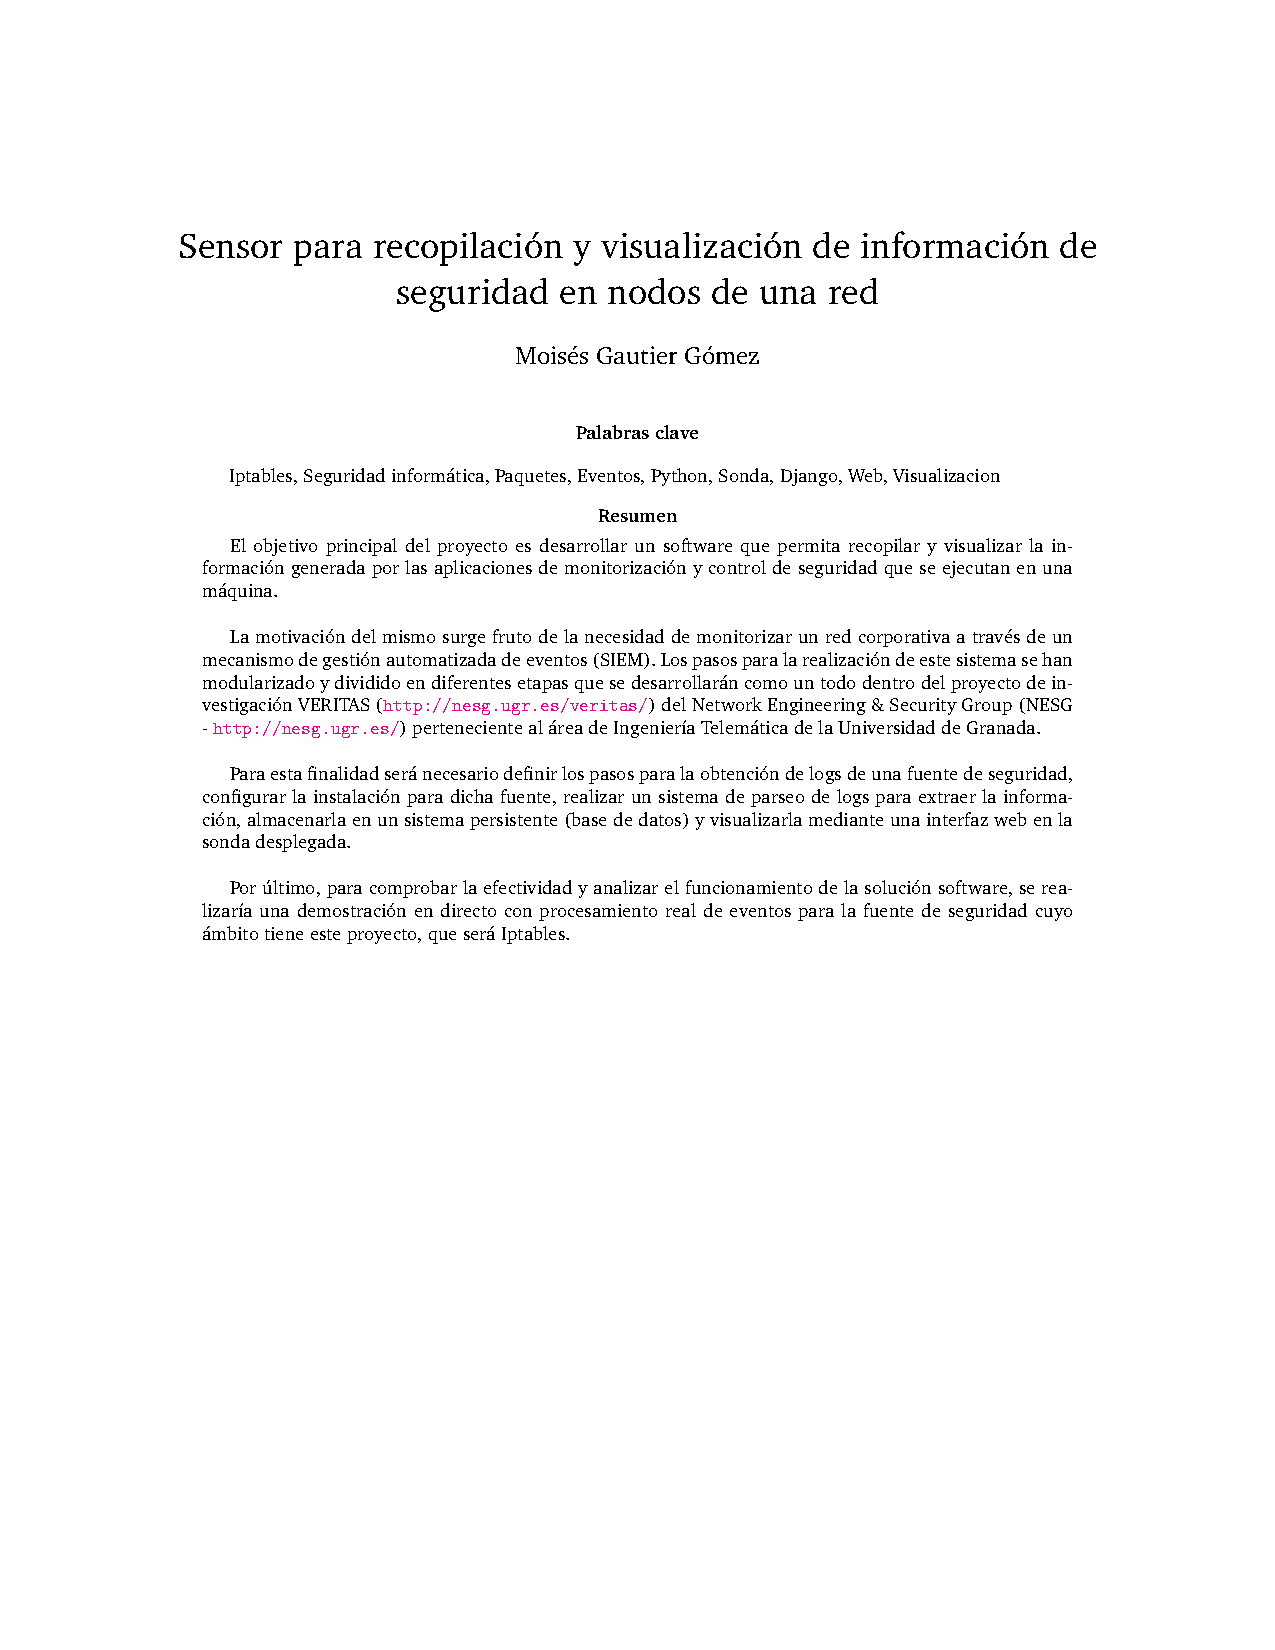
\includepdf[pages=1-]{primerahoja.pdf}
\cleardoublepage

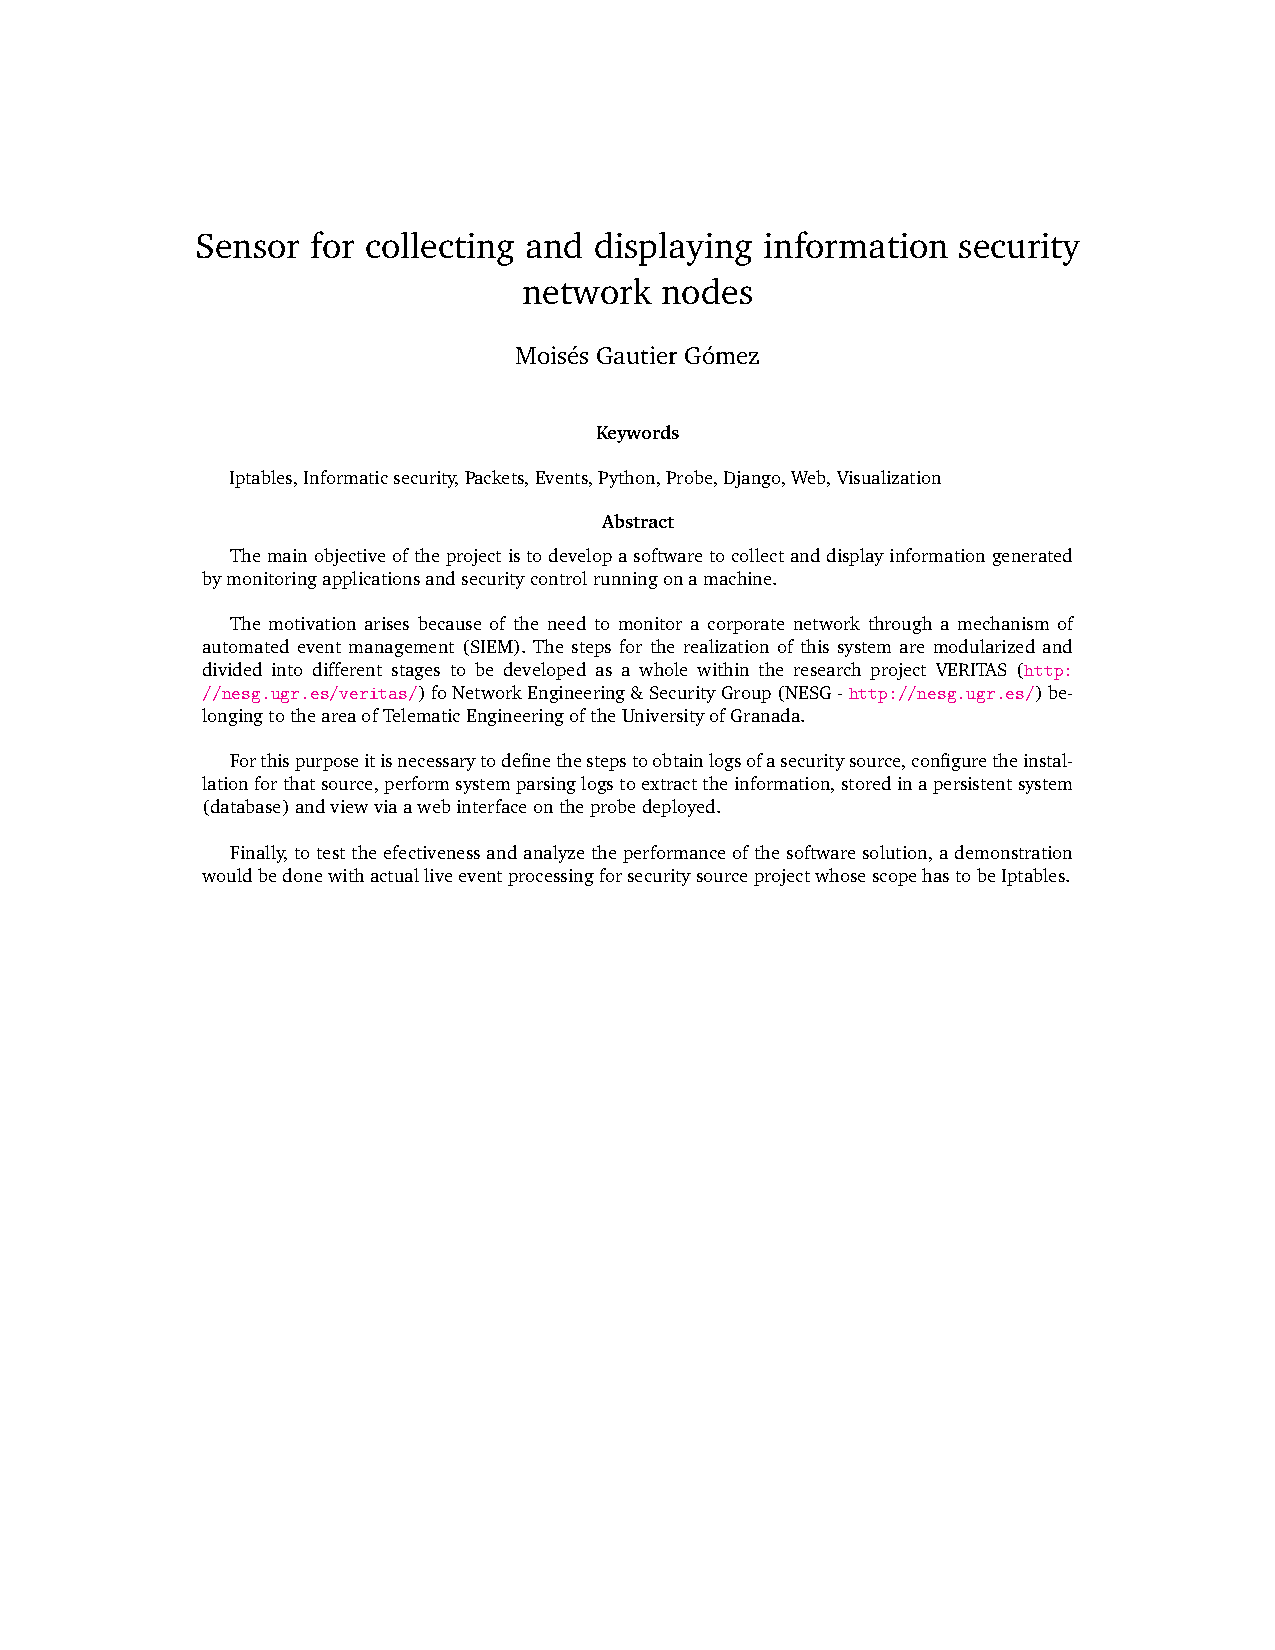
\includepdf[pages=1-]{primerahoja-en.pdf}
\cleardoublepage

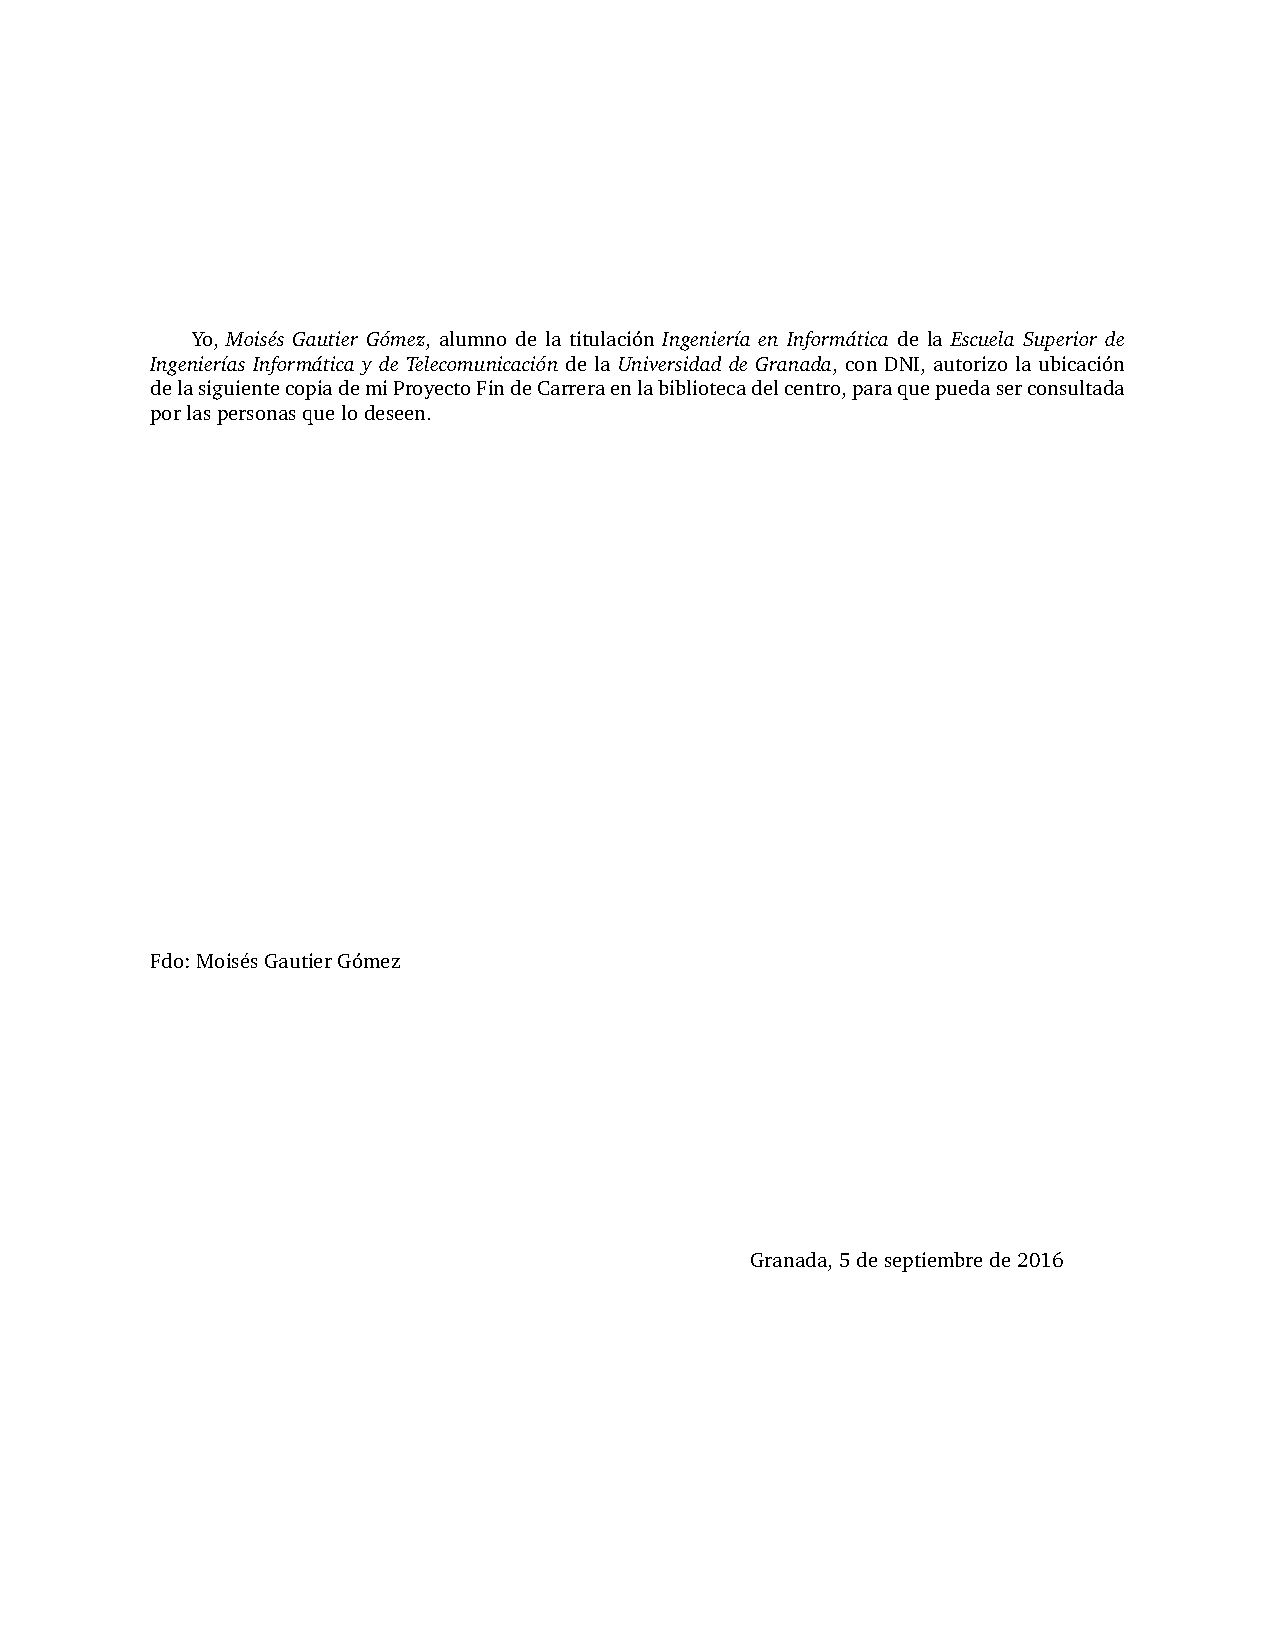
\includepdf[pages=1-]{autorizacion.pdf}
\cleardoublepage

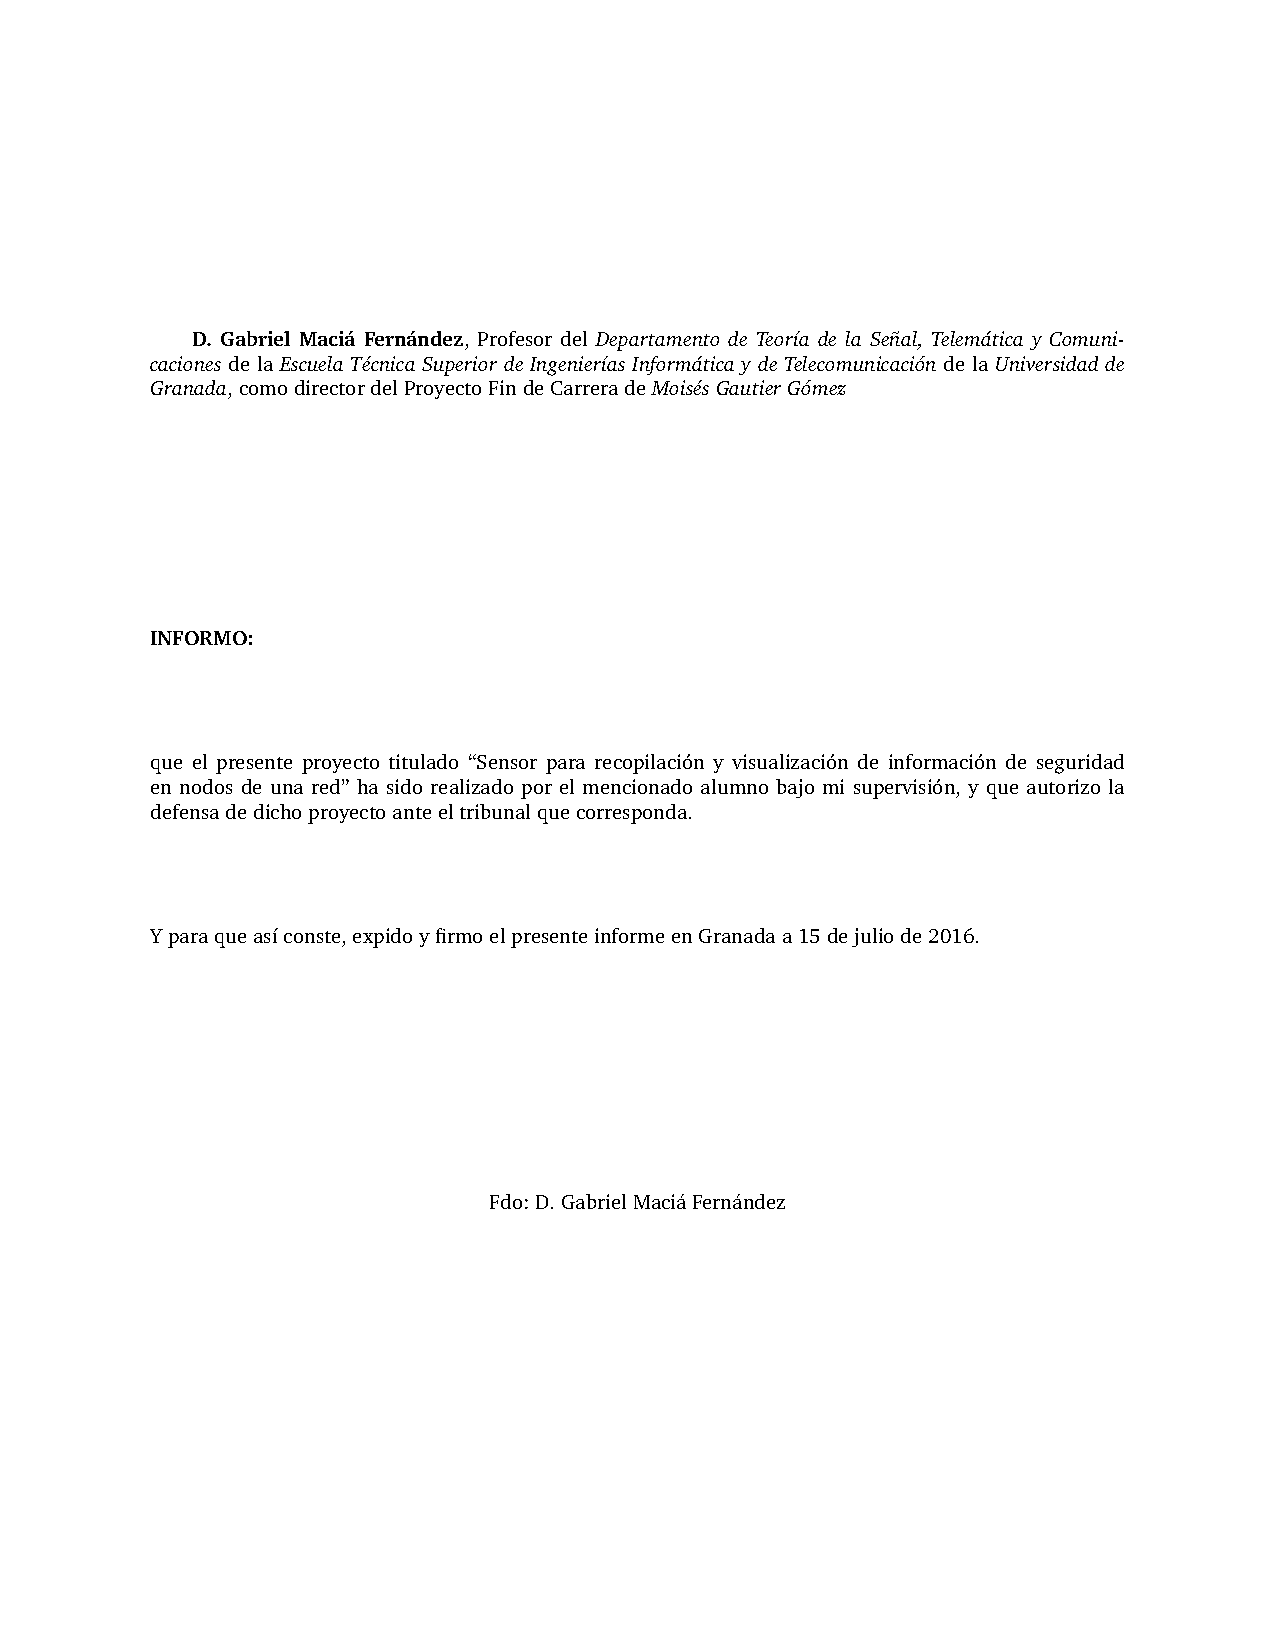
\includepdf[pages=1-]{tutor.pdf}
\cleardoublepage

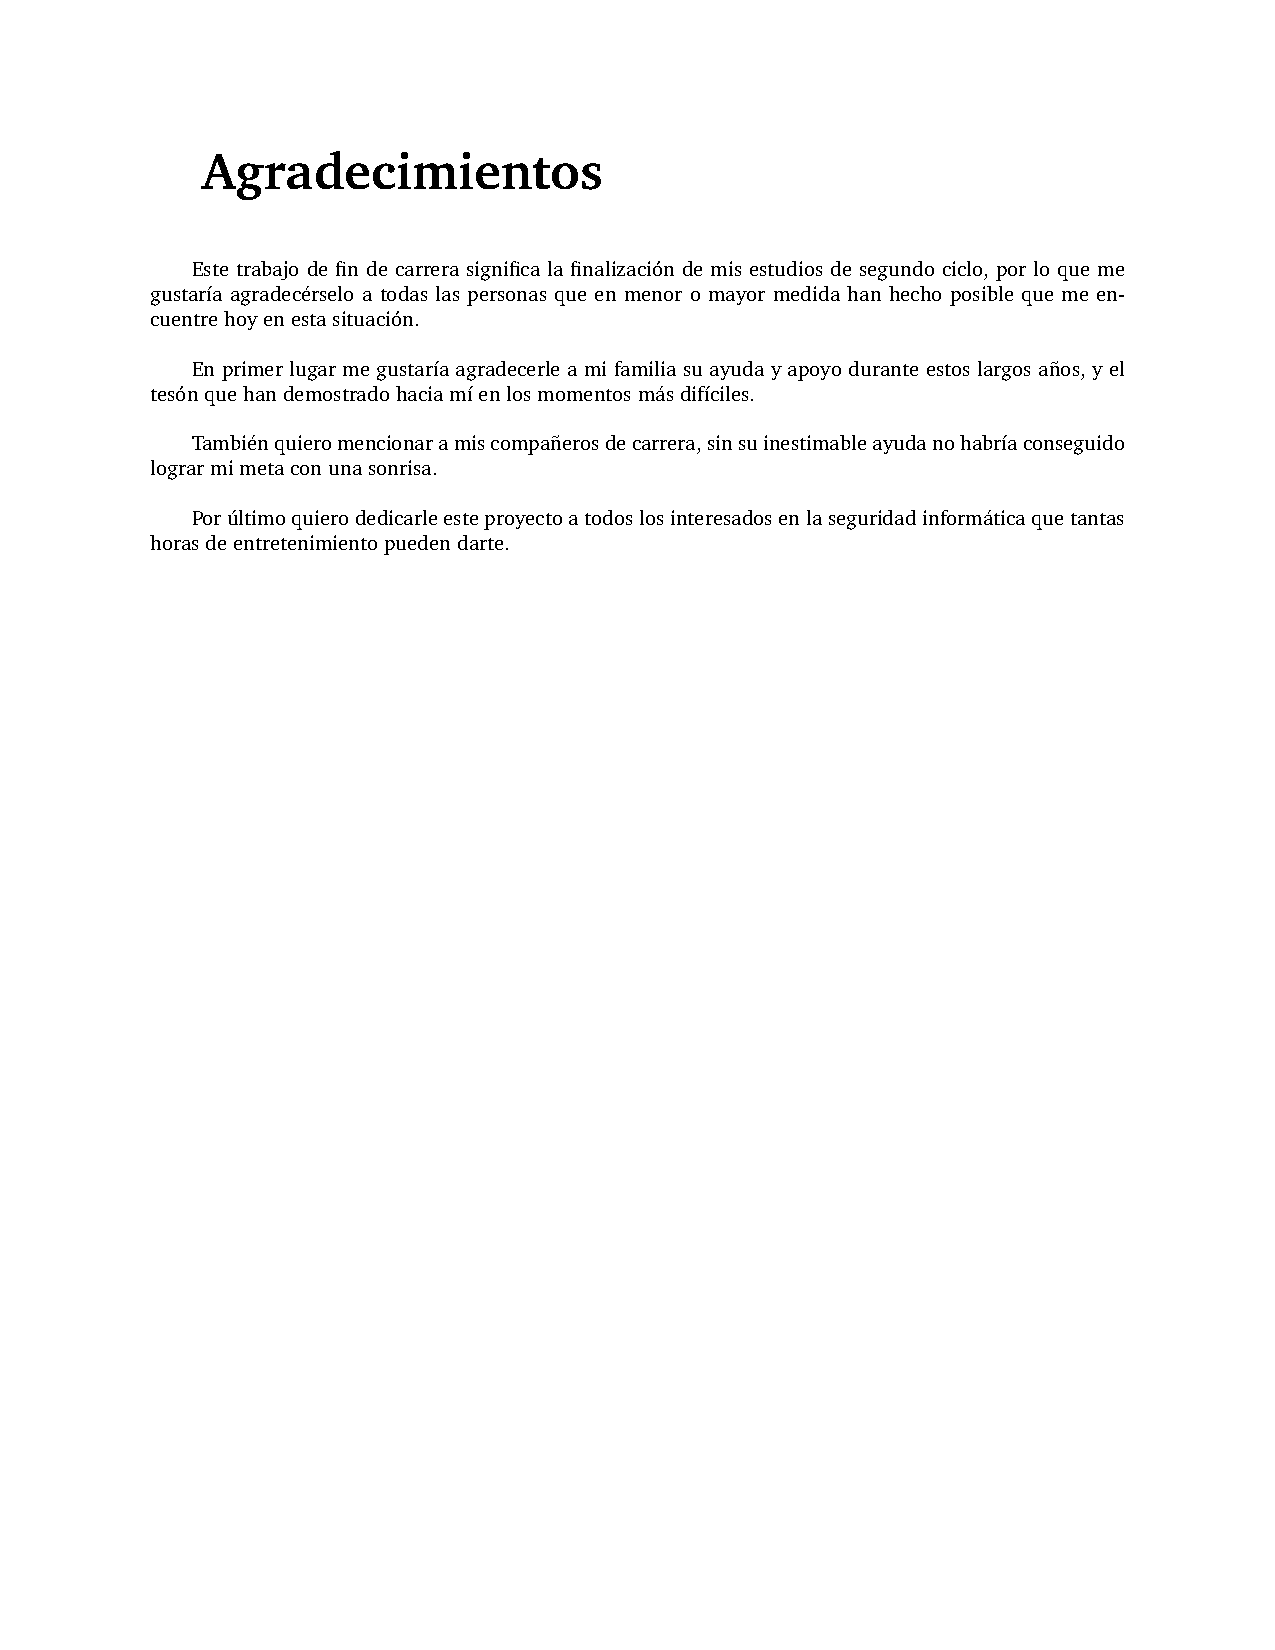
\includepdf[pages=1-]{agradecimientos.pdf}
\cleardoublepage

{\huge \textbf{Licencia}}
\\
\\
\small{Este documento ha sido liberado bajo Licencia GFDL 1.3 (GNU Free Documentation License). Se incluyen los términos de la licencia en inglés al final del mismo.\\

Copyright \copyright{} 2016 Moisés Gautier Gómez. Permission is granted to copy, distribute and/or modify this document under the terms of the GNU Free Documentation License, Version 1.3 or any later version published by the Free Software Foundation; with no Invariant Sections, no Front-Cover Texts, and no Back-Cover Texts. A copy of the license is included in the section entitled "GNU Free Documentation License".\\}

\cleardoublepage

\frontmatter

%\section*{Agradecimientos}

<agradecimientos>----</agradecimientos>

\cleardoublepage

\section*{Licencia}

<licencia>-----</licencia>

\cleardoublepage

\section*{Notación y formato}

<notacion>------</notacion>

\cleardoublepage

\tableofcontents
\listoffigures
\mainmatter

\pagestyle{fancy}
\fancyhead[LE,RO]{\rightmark}
\fancyhead[LO,RE]{\slshape \leftmark}
%\fancyroot[C]{\thepage}

\chapter{Introducción}
\label{chap:introducción}

\emph{Estar preparado para la guerra\\ es uno de los medios más eficaces\\ para conservar la paz\\ George Washington}\\

En el siglo XXI todo pasa por ser digital y si no, ya es que lo era antes de llegar a este punto. Quizás muchas de las tecnologías que hoy conocemos se basen en un sistema informatizado, ya sea en su formato de software o sistema embebido. Y es que todo pasa por ser una herramienta software diseñada para un propósito en concreto: un mecanismo de apertura de puertas mediante tarjetas RFID, procedimientos industriales o aplicados a alguna infraestructura crítica o de bien común, una aplicación del tiempo en tú terminal móvil, el propio sistema operativo con el que se puede éste el documento, etc. \\

Hay un sinfín de aplicaciones software que hacen nuestro día a día más llevadero y más fácil. Pero hay un punto que no todos conocen y es la necesidad de saber como se ha creado ése producto o como funciona realmente por su interior. En ese interior, a veces, podemos encontrar cosas que no estaban predestinadas a tener ese comportamiento y debido a ése comportamiento anómalo o imprevisto se generan situaciones de incertidumbre en las que el ser humano debe estar capacitado para afrontarlas. Dichas situaciones se suelen conocer con el término anglosajón de ``bug'' y sobre los bugs hay una especial categoría que se denominan fallas de seguridad o critical/several bugs. \\

Estas situaciones no previstas provocan que nuestro sistema, sea el que fuese, actúe de forma inesperada ante un input de información permitido o legítimo permitiendo un uso inadecuado de los recursos a los que se acceden mediante la aplicación. De este concepto o problema, surge en gran medida, el término de seguridad informática el cuál intenta abarcar y dar solución a estos problemas que pueden ir desde un simple fallo de desarrollo, a un fallo crítico que comprometa la seguridad o confidencialidad de los documentos de una empresa o gobierno. \\

Debido a esta problemática, surge la necesidad de analizar, monitorizar y generar sistemas de seguridad perimetral que permita a las empresas ver que tipo de tráfico interno se genera, que tipo de tráfico externo tiene y cómo se hace uso de él (navegación hacia el exterior, tuneles VPN, conexiones remotas a dispositivos, etc). Así pues, se podría decir que para obtener este tipo de eventos sobre protocolos, tráfico, DNS, IPs, VPNs,.. se tienen que configurar dispositivos de seguridad para la recolección de estos tipos de inputs o fuentes. \\

Una de las fuentes más conocidas dentro del mundo de la informática es el firewall, pero no así de las de un uso más extendido dentro del mundo doméstico sino el comercial o corporativo. Y dentro de los muchos tipos de software enfocados a tráfico (firewall) se encuentra el paquete de las distribuciones GNU/Linux: Iptables (software fruto del proyecto Netfilter para el kernel de GNU/Linux). Con esta herramienta se pueden definir políticas de filtrado de tráfico para cualquier tipo de protocolo TCP/UDP que queramos limitar entre el exterior y nuestra máquina y viceversa. Además, estas políticas nos permiten derivar dicho tráfico a archivos que podemos manipular obteniendo así los eventos que representan al tráfico generado por una máquina conectada a una red, que posteriormente podemos manipular para generar estadísticas o tipos de uso para una red. \\

\section{Contexto: Seguridad informática}

La seguridad informática es el proceso de mantener un aceptable nivel de percepción frente a un riesgo. Así pues ninguna organización se puede considerar ``segura'' en cualquier momento, más allá de la última comprobación que se realizo dentro de su política de seguridad.\\

Un proceso seguro se encuadra dentro de las siguientes 4 etapas: Evaluación, Prevención, Detección y Respuesta:

\begin{itemize}
\item Evaluación: es la preparación para las otras 3 etapas. Se considera como una acción separada porque se relaciona con las políticas, procedimientos, leyes, reglamentos, presupuestos y otras funciones de gestión, además de la propia evaluación técnica enfocada a la seguridad. No tener en consideración estos supuestos anteriores, podría dañar las etapas del diseño.
\item Prevención: es la aplicación de contramedidas para reducir la probabilidad de tener una situación comprometida.
\item Detección: es el proceso de identificación de intrusiones. Una intrusión se puede considerar como una violación de una política de seguridad o como un incidente de seguridad a nivel de software/dispositivo.
\item Respuesta: es el proceso de validar los inputs recogidos por la detección para tomar medidas que solucionen las intrusiones. El primer enfoque que debemos realizar consiste en restaurar la funcionalidad dañada y seguir recopilando información para tener claras las evidencias del atacante sobre nuestro sistema y poder así emprender las acciones legales que correspondan.
\end{itemize}

De estas etapas anteriores haremos incapié en la etapa de detección que es en la que se enmarca el ámbito de este proyecto. Dado que el principal objetivo es facilitar la monitorización de la información de seguridad.

\section{Motivación y objetivos del proyecto}

El objetivo principal del proyecto es desarrollar un software que permita recopilar y visualizar la información generada por las aplicaciones de monitorización y control de seguridad que se ejecutan en una máquina.\\

La motivación del mismo surge fruto de la necesidad de monitorizar una red corporativa a través de un mecanismo de gestión automatizada de eventos. Los pasos para la realización de este sistema se han modularizado y dividido en diferentes etapas que se acometarán como un todo dentro del proyecto de investigación VERITAS (\url{http://nesg.ugr.es/veritas/}) del Network Engineering \& Security Group (NESG - \url{http://nesg.ugr.es/}) perteneciente al área de Ingeniería Telemática de la Universidad de Granada.\\

\section{Estructura de la memoria}

En cuanto a la estructura de esta memoria del proyecto final de carrera, tras este capítulo dónde se presentan los objetivos y la visión en general del proyecto, se expone el estado del arte y el análisis de requisitos previos al desarrollo software.\\

En el capítulo siguiente, veremos la etapa del diseño de software así cómo posterior evaluación del mismo.\\

Finalmente, se presentan las conclusiones generales obtenidas una vez realizado el proyecto, como también la planificación del mismo y estimación de costes.\\

Además, se presentan las referencias bibliográficas donde se incluyen las fuentes consultadas para la elaboración de este proyecto, un resumen que engloba las generalidades fundamentales de la aplicación, una guía de utilización (manual de usuario), una guía de instalación, un compendio del software utilizado para el desarrollo y otro de los lenguajes de programación, y finalmente, la licencia completa del documento.\\


\chapter[Arte]{Estado del arte y tecnologías utilizadas}
\label{chap:estado del arte}

\section[Estado del arte]{Estado del arte de herramientas para monitorizar información}

En primer lugar, se realiza un estado del arte de herramientas que pudieran realizar funcionalidades parecidas a las que se van a implementar en este proyecto.\\

Actualmente existen diversos tipos de herramientas que realizan tareas de recolección, filtrado y gestión de eventos dentro un sistema. Las que se han podido analizar y comprobar han sido las siguientes:

\subsection{Lookwise}
\hspace*{1.7in}{
\includegraphics[scale=0.5]{diagramas/lookwise-logo.png}}\\

Lookwise es una herramienta corporativa que hace las funciones de SIEM en materia de gestión de seguridad, Big Data y cumplimiento normativo (ISO/LOPD y PCI DSS).

\subsubsection{Características}

Gestión centralizada
\begin{itemize}
\item Interfaz gráfica de administración y operación centralizada.
\item Creación y distribución de políticas de forma remota.
\item Integración de alertas y explotación de resultados.
\item Cuadro de mandos de seguridad.
\item Visibilidad en base a roles y permisos.
\item Integración con sistemas SIEM.
\end{itemize}

Comunicaciones
\begin{itemize}
\item Autenticadas y cifradas
\item Ininterrumpidas
\item Comprimidas
\end{itemize}

Plataformas soportadas
\begin{itemize}
\item Familia Windows XP (Windows Kernel 5)
\item Familia Windows 7 (Windows Kernel 6)
\end{itemize}

Arquitectura
\begin{itemize}
\item Arquitectura Distribuida.
\item Arquitectura Modular.
\item Flexible y escalable.
\item Balanceo de carga.
\item Despliegue remoto de funcionalidades y actualizaciones.
\end{itemize}
\begin{figure}[H]
\hspace*{-0.25in}{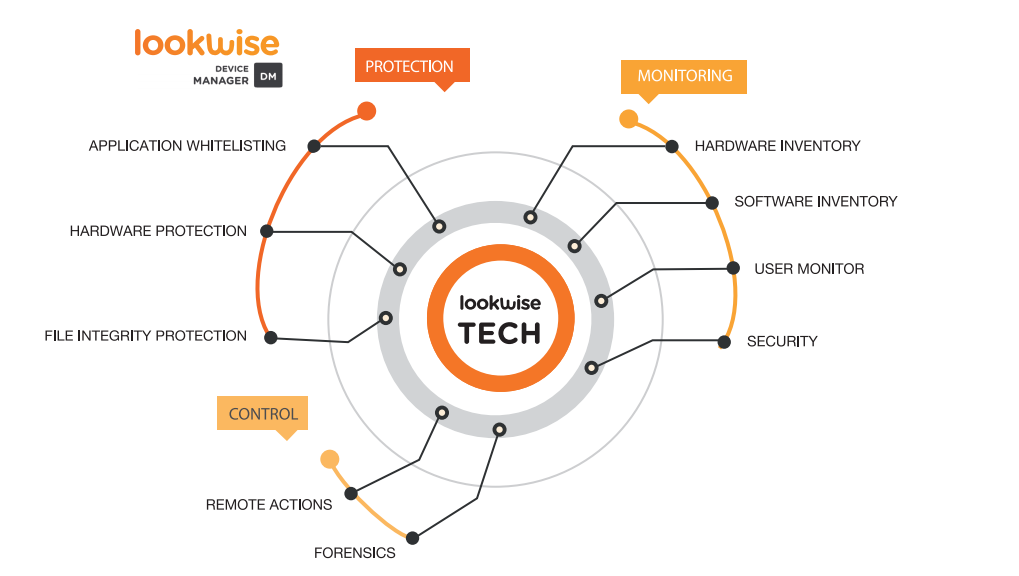
\includegraphics[scale=0.5]{diagramas/funcionalidades-lookwise.png}}
\caption{Funcionalidades Lookwise}
\end{figure}

\subsubsection{Análisis de la herramienta}

La herramienta de análisis de incidencias y vulnerabilidades hace la mismas funcionalidades de un SIEM pero con una capa más enfocada al cumplimiento del estándar de seguridad de datos de cuentas bancarias - PCI DSS (Payment Card Industry Data Security Standard - \url{https://es.pcisecuritystandards.org/minisite/en/}) y de infraestructuras críticas. Gestiona eventos del sistema y los correla con alertas predefinidas internamente o que se hayan incluido cómo especificación del cliente. Detecta fallos en el Active Directory y nos genera un sistema de informe con las incidencias más graves de cara a la parte de consultoría de incidentes por parte el equipo interno.


\subsection{ELK Stack}

La pila ELK se basa en una solución open-source de tres productos bien diferenciados que se relacionan entre sí (en resumidas cuentas se trata de un SEM) de la siguiente manera:

\begin{figure}[H]
\hspace*{.5in}{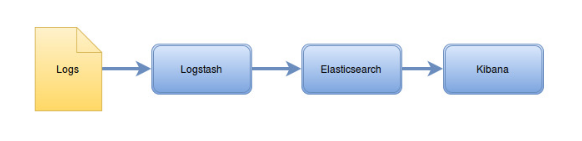
\includegraphics[scale=0.65]{diagramas/elk-stack.png}\\}
\caption{ELK Stack ~\cite{11}}
\end{figure}

\begin{itemize}
\item Logstash para el registro centralizado de logs y su posterior normalización y enriquecimiento de datos.
\item Elasticsearch para la búsqueda de datos y análisis en profundidad de un sistema.
\item Kibana cómo herramienta de visualización de los datos recolectados y procesados anteriormente según las especificaciones que queramos para el filtrado.
\end{itemize}

\subsection{Logstash}
\begin{figure}[H]
  \hspace*{1.75in}{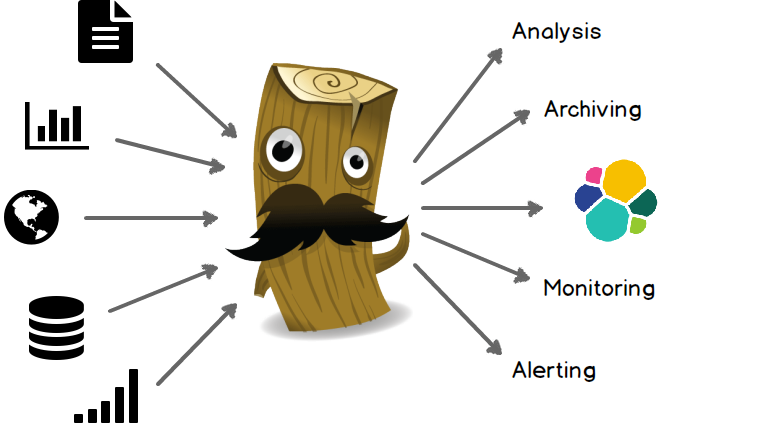
\includegraphics[scale=0.25]{diagramas/logstash.png}\\}
  \caption{Logstash description}
\end{figure}
Logstash es un motor open-source de recopilación de datos con capacidad de multihebrado en tiempo real. Esta herramienta puede unificar dinámicamente datos de diferentes fuentes y normalizar dichos datos para los outputs de nuestra elección. Además nos permite filtrar y discretizar todos los datos recolectados para obtener información analítica que pueda ser visualizada.\\

\begin{figure}[H]
  \hspace*{.5in}{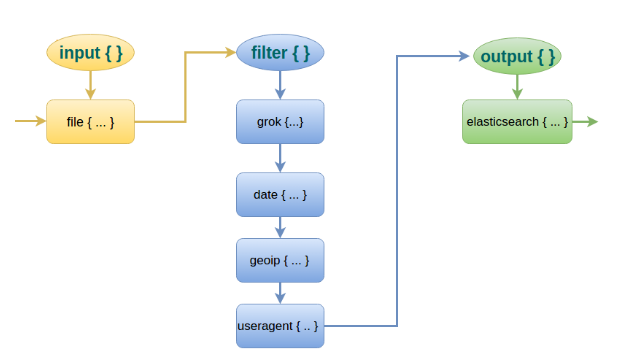
\includegraphics[scale=0.65]{diagramas/logstash-configuration.png}\\}
  \caption{Diagrama de flujo interno de logstash ~\cite{11}}
\end{figure}

Con logstash, cualquier tipo de evento puede ser enriquecido y transformado con un amplio repertorio de inputs/filtros y los datos de salida, se pueden modificar dependiendo del tipo de software sobre el que queramos introducir esos datos (plugins y códecs).\\

\subsection{Elasticsearch}
\hspace*{2in}{
\includegraphics[scale=0.15]{diagramas/elasticsearch-logo.png}\\}
Elasticsearch es un motor open-source de búsqueda y análisis de información de gran escalabilidad. Esta herramienta permite almacenar, buscar y analizar grandes volúmenes de datos de forma rápida y en tiempo real. Se suele utilizar cómo motor/tecnología subyacente de otras aplicaciones (wrapers), permitiendo así realizar funciones de búsqueda complejas de una manera más ágil.\\

\subsection{Kibana}
\hspace*{2.25in}{
\includegraphics[scale=0.75]{diagramas/kibana-logo.png}\\}
Kibana es una plataforma open-source de análisis y visualización de datos diseñada para trabajar con Elasticsearch. Kibana se utiliza para buscar, ver e interactuar con datos almacenados en los índices o base de datos de Elasticsearch. De esta forma se puede realizar fácilmente un análisis avanzado de datos que permita visualizarlo en una gran variedad de gráficas, tablas y mapas.\\

Kibana hace que sea fácil de entender y procesar grandes volúmenes de datos. Mediante su interfaz basada en un cliente web, nos permite crear de forma simple y ágil filtros sobre los datos extraidos mediante consultas a la bd de Elasticsearch en tiempo real.\\


\subsection{Análisis de la herramienta}

La pila ELK, cómo bien se ha comentado en los tres puntos anteriores nos permite recolectar, procesar y correlar cualquier tipo de logs que genere nuestro sistema de una manera visual, ágil y fácil de entender. \\

El motor de indexación de datos, Elasticsearch, nos permite obtener una ejecución en tiempo real de los logs del sistema así cómo poder escalar dicho volumen de datos dependiendo de la situación. El único inconveniente de esta herramienta es que el sistema de referenciación de documentos internos es mediante json. Es un formato muy versátil pero incapaz de tener funcionalidad por si sola.\\

Después tenemos Logstash que es el encargado de hacer de middleware entre elastic y kibana, es decir, la parte de la recogida de muestras/eventos y la parte dónde se visualizan esas muestras. Logstash hace de filtro y de motor de normalización de datos entre los diferentes activos que tiene asignados para así poder tener todos los datos unificados según la especificación que queramos dar a cada uno de ellos. \\

Cada parte de la pila esta desarrollada en su propio lenguaje de desarrollo, siendo Java (o Groovy) el lenguaje de desarrollo de elastic, Ruby el de logstash y Javascript para Kibana. El único inconveniente que se ha podido observar es que la solución ELK está diseñada para trabajar más optimizada en entornos de cloud computing y no de manera local en un servidor. Dado que tendría que usar recursos propios de la máquina y conforme se vayan escalando nuevos recursos estos irán aumentando los de la máquina. Si hay limitación de hardware por los mismos puede llegarse a experimentar un cuello de botella entre elastic y kibana, siendo la carga de datos muy lenta y con tiempos de refresco bastante altos. \\

\section[SIEM]{Sistemas de gestión de información y eventos de seguridad: SIEM}

Un sistema de gestión de información y eventos de seguridad, es un concepto que se suele usar para referirse a dos tecnologías que unifican el concepto como son SEM y SIM. \\

SEM (Security Event Management), tiene como principal funcionalidad la de recolectar, procesar y almacenar los eventos de seguridad que ocurren en una máquina; y SIM (Security Information Management) se suele usar para la correlación de eventos y obtención de una normalización de los mismos para un posterior análisis, procesamiento mediante algún tipo de técnica estadística o matemática, generado de informe sobre los datos que se han obtenido en la etapa del SEM, etc. \\

Así pues, el término SIEM haría referencia a la recopilación de eventos de seguridad y otros relacionados para su documentación y análisis. La mayoría de estos sistemas trabajan mediante la implementación de varios agentes en una tipología jerárquica en la que cada nivel de la jerarquía cumple con un cometido a menor escala dentro del sistema de seguridad definido (máquinas de usuarios, servidores, equipos en red, firewalls, antivirus, etc). Los agentes reenvian dichos eventos a una consola de gestión centralizada, que realiza inspecciones sobre los mismos y asigna la criticidad correspondiente. \\

\begin{figure}[H]
  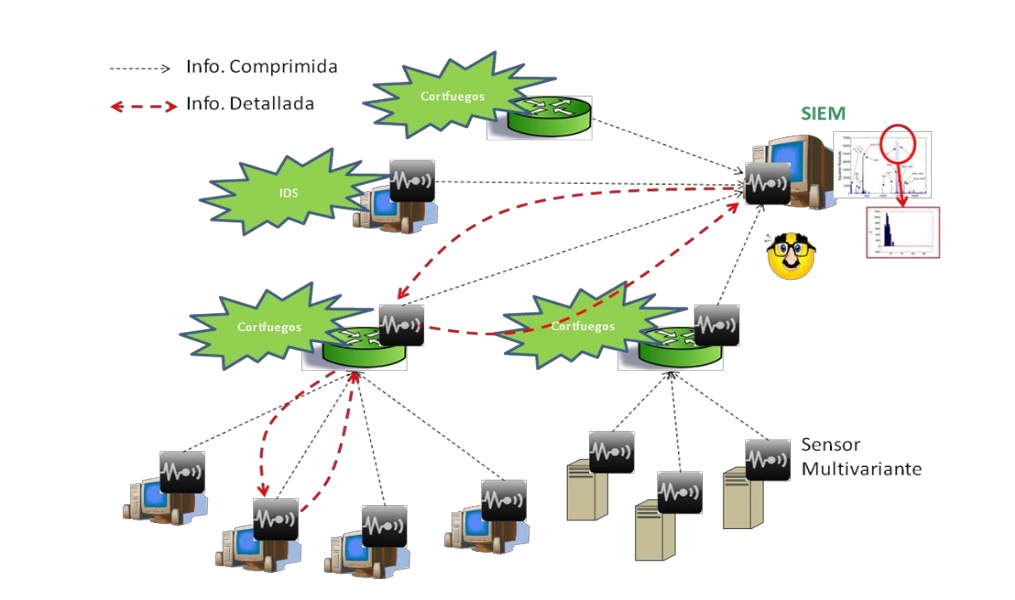
\includegraphics[scale=.4]{diagramas/siem.png}
  \caption{Sistema SIEM multivariante distribuido - Proyecto \href{http://nesg.ugr.es/veritas}{VERITAS}}
\end{figure}

\subsection{Principales características}

Estos son los puntos que principalmente gestiona un SIEM:\\

\begin{itemize}
\item Gestión de parches (actualizaciones) del kernel o software de terceros cómo adobe, java, etc.
\item Antivirus en máquinas de usuarios o en servidor.
\item Gestión de cortafuegos.
\item Integración con Active Directory (LDAP).
\item Sistema de prevención de intrusiones (en red: NIPS / basado en hosts: HIPS)
\item Proxy / Filtro de contenidos
\item Email: anti-spam / anti-phishing
\item Análisis de vulnerabilidades
\item Herramientas de seguridad opcionales:
  \begin{itemize}
  \item IPS para redes Wifi.
  \item Control de firewall web.
  \item Aplicaciones que monitoricen bases de datos.
  \item Prevención de pérdida de datos.
  \item Gestión de riesgos y herramienta de cumplimiento de políticas
  \end{itemize}
\end{itemize}

\subsection{Análisis}

Aunque esta herramienta sea como un conglomerado de aplicaciones o herramientas de detección y análisis, su puesta en marcha no es así tan fácil como cabría esperarse dado que cada despliegue requiere de unos activos o fuentes diferentes. Además, cada solución final requerirá de unas especificaciones distintas, con lo que su implantación depende en gran medida de la facilidad de adaptación al entorno y también de que los responsables de dicha herramienta tengan un profundo conocimiento sobre ella.\\

Una de las palabras más comunes que definen la implementación de un SIEM es: desalentador. A menudo termina costando más de lo previsto, requiere una experiencia sobre la herramienta que a menudo suele ser externalizada (sobre el propio fabricante) y puede llevar un tiempo considerable antes de obtener resultados tangibles.\\

Los motivos para los que generalmente se introducen éste sistema en la red corporativa suelen ser varios, pero entre los más destacados suelen ser: el cumplimiento de una normativa industrial o de un gobierno, la gestión de incidentes recurrentes de seguridad o también que en la licitación de un contrato esté contemplado la puesta en marcha de este sistema para una mayor calidad del servicio prestado por un tercero o por la propia entidad. Y aún así, que la propia empresa ya gestione sus eventos internos o los monitorice, no implica que su migración al SIEM sea inmediata.\\

Además, la licitación o adquisición de un producto de estas características supone que el entorno sobre el que se va a aplicar contiene dispositivos de seguridad que monitorizar (sino se está realizando dicho control), que se dispongan de herramienta de centralización de datos (físicamente o en cloud) y que se quiera un sistema de gestión 24/7, incluido la monitorización fuera de horario laboral.\\

Son estas razones por las que a veces un sistema tan complejo y gigantesco puede que genere un sobrecoste o cubra pocas áreas de la red en las que no se tiene necesidad de vigilar. Siendo esto un incoveniente finalmente, dado que hay otras herramientas (de las que se nutre el SIEM) que ya cumplen con dicha funcionalidad a coste de tener un sistema muy pesado que gestionar.\\

\subsection{Otros SIEM comerciales}

Existen otras muchas más herramientas, comerciales en su gran mayoría, que tratan de abordar el concepto de SIEM a un paso más allá de lo anteiormente analizado. A continuación se van a citar algunas de esas herramientas:

\begin{itemize}
\item \href{https://www.alienvault.com/products/ossim}{OSSIM} - Alienvault: Herramienta SIEM de código abierto.
\item \href{http://www8.hp.com/es/es/software-solutions/siem-security-information-event-management/}{HPE Arsight SIEM} - HP: Herramienta SIEM privativa.
\item \href{http://www-03.ibm.com/software/products/es/qradar-siem}{IBM Security QRadar SIEM } - IBM
\item \href{http://www.splunk.com/es\_es}{Splunk}
\item \href{https://logrhythm.com/es/}{LogRhythm}
\end{itemize}

\section{Solución tecnológica de éste proyecto}

La principal diferencia que existe entre éste proyecto final de carrera y las herramientas anteriormente analizadas es que el desarrollo y gestión de la información no se hace de forma analítica sino que se gestionan cantidades de datos (en la fase de recolección de logs de dispositivos) y estos no reciben ningún tipo de filtro o procesamiento previo. Se transportan desde el dispositivo monitorizado a otro en dónde se correlan los distintos logs o recolecciones según patrones definidos por los ingenieros de seguridad de la compañía encargada de detectar anomalías en los mismos. \\

No existe ningún tipo de mecanismo analítico de esta información dado que el punto de inflexión o la inteligencia, está en las etapas finales y no en las previas del tratamiento de la información. Para dotar de una mayor funcionalidad a estos sistemas hay extensiones o módulos que desarrollan las compañías que amplian la capacidad analítica de la misma por una cantidad económica bastante alta y su uso suele estar supeditado a licencia. \\

Además, la visualización de los eventos almacenados no siempre es inmediata y necesita de otra aplicación externa o módulo (funcionalidad extra) que explote estos recursos y los haga fácil para la interacción humana.\\

\newpage
\section{Tecnologías utilizadas}

A continuación se detallan las diferentes tecnologías/bibliotecas/lenguajes que se han empleado para la elaboración del proyecto y por qué se han escogido por encima de otras posibles soluciones.

\subsection{Python}

\hspace*{1.2in}{
\includegraphics[scale=0.4]{diagramas/python-logo.png}}

Web: \url{https://www.python.org/}\\

Python es un lenguaje multiparadigma cuya estructura principal está integramente basada en objetos con sus diferentes métodos y atributos internos. Además también posee tipado dinámico, recolector/administrador de la memoria interna y un sistema de referenciado interno de atributos. \\

Las principales características que han favorecido su elección fueron:
\begin{itemize}
\item Es un lenguaje que facilita la implementación de una forma muy ágil y dinámica.
\item Su sistema de paquetes es muy intuitivo y ligero. Se puede instalar cualquier dependencia descargandola del repositorio de paquetes PyPi en el que se pueden encontrar infinidad de soluciones software dependiendo de lo que necesites. Sino, siempre se puede definir el propio paquete software y subirlo al repositorio.
\item Es de licencia similar a la BSD (Python Software Foundation License) compatible con la GNU GPL. Por lo tanto se puede modificar cualquier aspecto del kernel del lenguaje o mejorar cualquier funcionalidad anteriormente definida.
\item Permite la fácil portabilidad entre plataformas, ya que sólo requiere de un intérprete que traduzca dicho código fuente a lenguaje máquina por lo que no existe una pesada fase de compilación por parte del sistema.
\item Tiene una amplia comunidad de desarrolladores y es muy fácil de aprender en un corto periodo de tiempo para alguien iniciado.
\item Es ampliamente empleado en el mundo de la seguridad informática para ser usado en parsers, procesadores de eventos y usos con la web cómo principal reclamo (Protocolos, paquetes, tráfico, etc).
\end{itemize}


\subsubsection{Python frente a otras soluciones}

En la fase de estudio de tecnologías, se planteo la posibilidad de desarrollar el proyecto con el lenguaje de programación Java pero se descarto por los siguientes aspectos:

\begin{itemize}
\item Precisa de unos conocimientos más avanzados sobre el control de procesos e hilos aunque sea más eficiente, también es más pesada la ejecución de los mismos en un sistema concurrente que puede que tenga muchos activos o fuentes que usar.
\item Lenguaje fuertemente tipado y muy estructurado.
\item Precisa de una compilación previa que pudiera incrementar los costes de empaquetar dicha solución y además solo se puede ejecutar en un entorno dónde exista una JVM o java virtual machine.
\item Para adaptar la solución obtenida a un resultado web tendría que hacer uso de un framework o IDE que ayudase a la hora de la gestión y diseño de la interfaz web así cómo la comunicación. En Python frameworks como Django, facilitan la tarea del despliegue en formato web y lo más cercano que se le parece es el lenguaje Groovy sobre el que se basa el software Elasticsearch.
\end{itemize}

\subsection{Procesos vs hilos}

En el proceso de desarrollo del proyecto hubo varios momentos en los que se valoró y estudió las difererencias entre un desarrollo software basado en procesos, a la hora de cada nuevo input que llegase a la monitorización, frente hilos o threads. A continuación, se hará un breve resumen sobre las diferencias entre ambos:

\subsubsection{Procesos}

Un proceso, se basa en la parte de un programa que se ejecuta en nuestro sistema, es decir, un conjunto de recursos reservados del sistema.

\subsubsection{Hilos}

Un hilo o thread, es similar a un proceso dado que hace uso de unos recursos reservados del sistema. Pero con una gran diferencia, porque si los procesos ocupan diferentes espacios de memoria, los hilos comparten ese espacio entre ellos.

\subsubsection{Problemas de los hilos}

La normal general es que un conjunto de hilos o procesos tiendan a compartir información entre ellos. Por lo que la solución de los hilos a priori parece ser la más adecuada dado que compartir información será mucho más fácil. Sin embargo, la compartición de grandes cantidades de información y haciendo un uso amplio de tareas concurrentes, pueden producir dos situaciones delicadas: el bloqueo mutuo (deadblock) y la condición de carrera (race condition).\\

\subsubsection{Hilos del kernel vs hilos del usuario}

Diferentes hilos comparten un mismo PID mientras que diferentes procesos, poseen sus propios PID. Sin embargo, esto no sucede a nivel de kernel. Los hilos del kernel tienen sus propios PID, debido a la forma en la que el kernel es ejecutado.\\

El kernel (para sistemas GNU) en sí mismo no se ejecuta cómo un proceso sino que sus tareas se ejecutan cómo parte de otros procesos. Debido a la gran cantidad de tareas que se ejecutan, en el kernel se realiza una implementación o acción alternativa para operar de forma similar a los procesos (esto es a lo que se le conoce cómo demonios).\\

\subsubsection{Solución que aplica Python}

A la hora de la implementación para comprobar que hilos se están ejecutando a través el hilo padre, se utiliza el método de la clase Thread enumerate.\\

Lo que se realiza en esa comprobación es que dentro de la pila o lista de thread que se han lanzado haya alguna coincidencia de objetos de la clase Iptables y si la hay ya existe un hilo previo en ejecución que hace las comprobaciones pertinentes.\\

\lstinputlisting{trozos-codigo/codigo-1.py}
\newpage
\subsection{Django}

\hspace*{1.9in}{
\includegraphics[scale=0.15]{diagramas/django-logo.png}}

Web: \url{https://www.djangoproject.com/}\\

Django es un framework web de alto nivel para el lenguaje de programación Python. Éste framework permite un despliegue de una aplicación de escritorio al entorno web de una forma sencilla, segura y fácilmente escalable. \\

Su metodología es MVT - Model View Template. A continuación, se explicarán en que consisten cada una de ellas:

\subsubsection{Model}

Model o Modelo es la parte encargada de la gestión con la base de datos y de abstraer su uso encapsulandola mediante clases que representan a cada una de las instancias de la BD (o tablas).\\

\subsubsection{View}

View o Vista es la parte encargada de la gestión entre la base de datos y el template. Puede llevar a confusión esta metodología de desarrollo web, ya que existe una similar: MVC. Pero en MVC (Model-View-Controller) el modelo se encarga de la gestión de la BD, la vista de representar los datos y el controlador de administrador o motor de contenidos entre la BD y la vista final de la aplicación web. \\

Así pues la \textbf{Vista} en el framework Django se representa al modelo MVC cómo el controlador.\\

\subsubsection{Template}

Template o Plantilla se refiere a la parte encargada de reprensentar la información almacenada en BD, procesada y generada mediante la Vista (View). Al contrario de un modelo MVC, en dónde el controlador se encarga de generar las vistas, en este modelo se representan las mismas cómo una plantilla de muchas otras que se van enrutando a diferentes funciones generadas por la vista. \\

Dicho esto, siempre habra una plantilla Master o padre de la que heredarán todas las hijas que vayamos asociando a nuestra web. Estas heredan una estructura o skeleton en formato html enriquecido con lenguaje propio de Django en formato python. Veamos un ejemplo de plantilla Master y una plantilla que se nutre de éste skeleton:\\

\lstinputlisting[language=HTML]{trozos-codigo/codigo-2.html}

En el fragmento de la plantilla Master incluimos los archivos estáticos del sistema (\textbf{load staticfiles}) y además especificamos dónde iría el cuerpo de las vistas o plantillas hijas que heredarán este skeleton mediante la especificación de un bloque (\textbf{block content} y \textbf{endblock}). Y ahora veremos un ejemplo de lo que podría ir dentro de ése bloque.\\

\newpage
\begin{minipage}{\linewidth}
  \lstinputlisting[language=HTML]{trozos-codigo/codigo-3.html}
  Aquí se observa perfectamente cómo se heredan las características de la plantilla Master y se define el bloque de contenido que en la plantilla Master ya se especificó (se situa dentro de las etiquetas \textbf{block} y \textbf{endblock}). \\
\end{minipage}

\subsection{C3js}

Web: \url{http://c3js.org/}\\

Es una biblioteca gráfica basada D3js, que es otra biblioteca visual en Javascript. En este caso, la biblioteca hace uso de la funcionalidad para gráficas de D3js adaptando su motor a otras posibles soluciones de implementación.\\

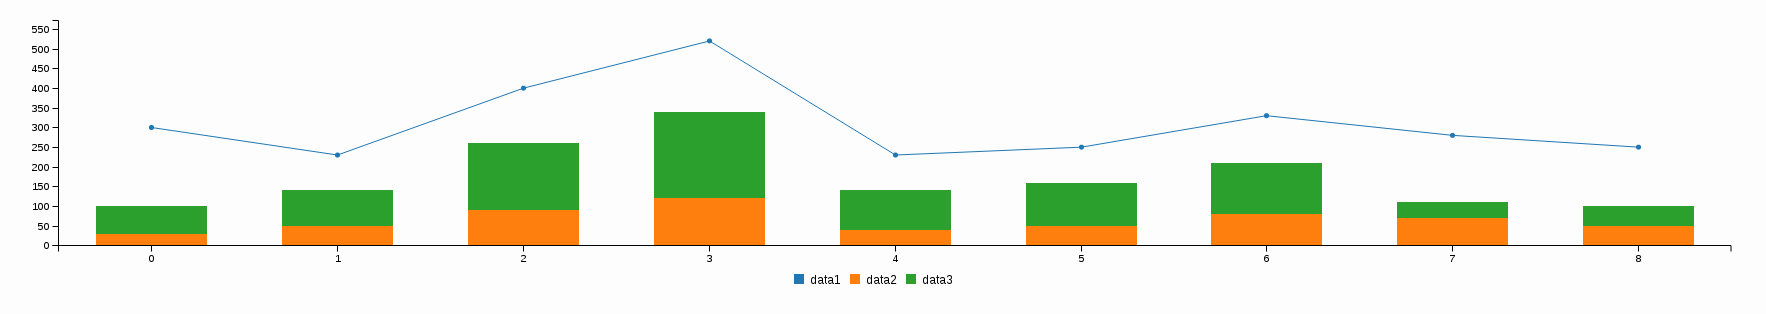
\includegraphics[scale=0.25]{diagramas/c3js-chart.png}

\subsection{D3js}
\hspace*{1in}{
\includegraphics[scale=0.35]{diagramas/d3js-logo.png}}

Web: \url{https://d3js.org/}\\

D3.js es una biblioteca javascript para la manipulación de documentos basado en datos. D3 nos ayuda a la hora de dar vida a los datos usando HTML, SVG y CSS de una forma sencilla y visualmente muy espectacular. Tiene su propio lenguaje que hace uso de las funcionalidades de Javascript por debajo y cuya comunidad es muy amplia en dónde podemos obtener multitud de ejemplos visuales que demuestran la capacidad de generación de gráficas y eventos de la biblioteca.\\

\begin{figure}[H]
  \hspace*{.6in}{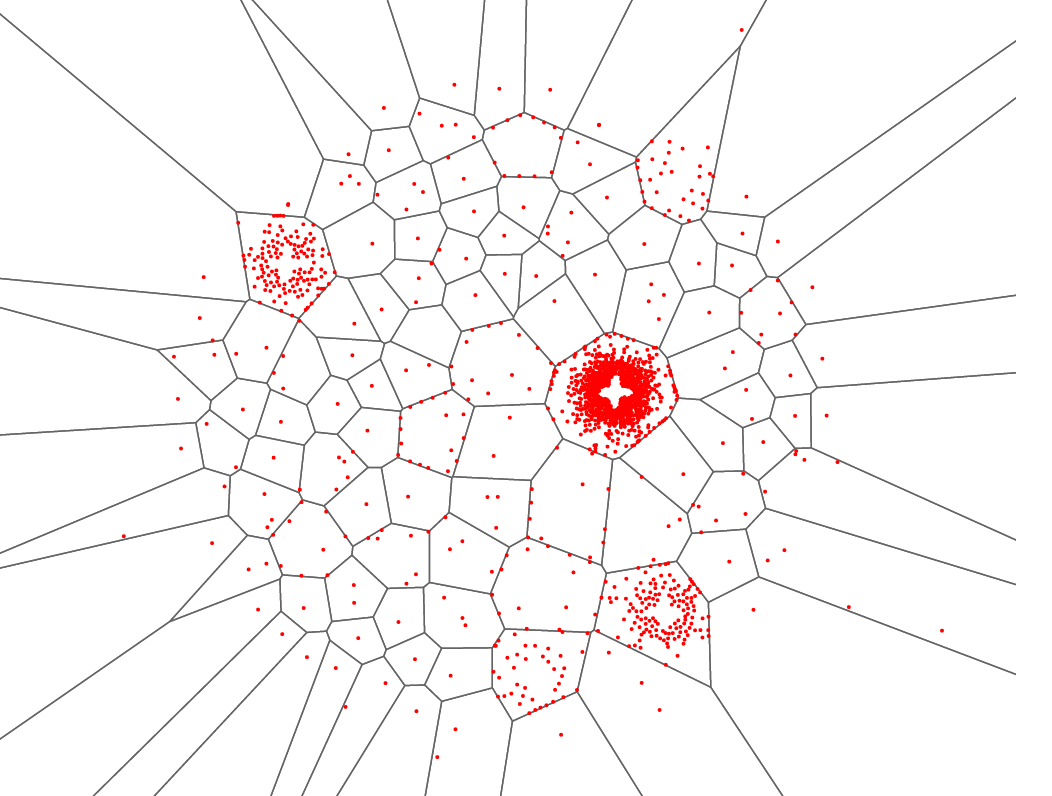
\includegraphics[scale=0.35]{diagramas/d3js-example.png}}
  \caption{Ejemplo de D3js}
\end{figure}


\subsection{\LaTeX}

Web: \url{https://www.latex-project.org/}\\

\LaTeX es un lenguaje de marcado que sirve para la redacción de documentos científicos o técnicos. Con esta herramienta o lenguaje se ha desarrollado la memoria actual del proyecto de final de carrera.

\subsection{Reactjs}

\hspace*{2.5in}{
\includegraphics[scale=0.15]{diagramas/Reactjs-logo.png}}

Web: \url{https://facebook.github.io/react/}\\

React es una biblioteca Javascript que permite construir interfaces de usuario en nuestra aplicación web. Existen soluciones similares a React cómo podría ser JQuery, pero en este caso el proceso de creación de componentes visuales se hace muy intuitiva mediante clases internas que encapsulan el contenido que posteriormente se traducirá a código Javascript nativo.\\

Para la traducción, React utiliza un componente llamada JSX, pero en nuestra solución se ha usado el paquete Babel (\url{https://babeljs.io/}) que es similar pero en formato Javascript y no NodeJS.\\

\subsection{Highcharts}

\hspace*{2in}{
\includegraphics[scale=0.35]{diagramas/highcharts-logo.png}}\\

Web: \url{http://www.highcharts.com/}\\

Highcharts es una biblioteca gráfica desarrollada en Javascript que permite construir gráficos de manera muy intuitiva, fácil, elegante y rápida. Dispone de una api documental muy práctica y que ayuda en su aprendizaje.\\

Con esta biblioteca se ha desarrollado la parte visual de la web en dónde se incluyen gráficas de eventos, eventos en tiempo real y estadísticas generadas por día.

\begin{figure}[H]
  \hspace*{-.05in}{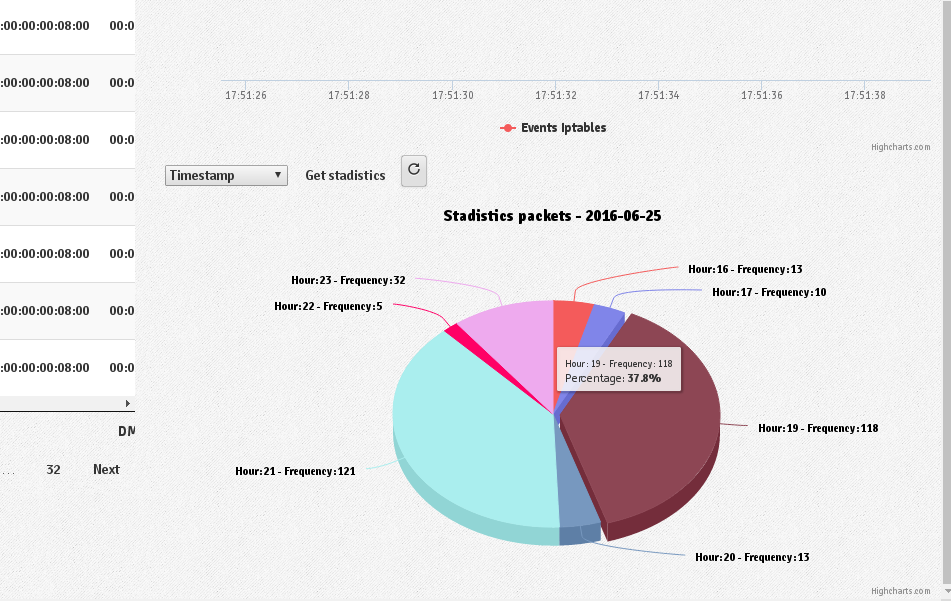
\includegraphics[scale=0.5]{diagramas/web_7.png}}
  \caption{Ejemplo de visualización para la biblioteca Highcharts}
\end{figure}

\subsection{SQLite}

\hspace*{2.25in}{
\includegraphics[scale=0.5]{diagramas/sqlite-logo.png}}

Web: \url{https://www.sqlite.org/}\\

SQLite es un biblioteca software que implementa un motor para bases de datos SQL. Sus principales características son las siguientes:

\begin{itemize}
\item Las transacciones de datos son atómicas, consistentes, aisladas y duraderas (ACID) incluso después de que el sistema tengo un fallo o se apague inesperadamente.
\item No necesita de una administración o configuración previa para su normal funcionamiento.
\item Implementación de un sistema SQL íntegro con características más avanzadas cómo indexación parcial.
\item La base de datos, en su totalidad, se almacena cómo un archivo normal en disco. Esto es útil para ser cargado directamente como un archivo en una aplicación.
\item Soporta bases de datos de Terabytes de tamaño y Gigabytes de string o archivos.
\item Facilidad de uso mediante su API interna.
\item No tiene ninguna dependencia externa.
\item Multiplataforma: Android, BSD, iOS, Linux, Mac, Solaris, VxWorks y Windows soportan este tipo de formato de base de datos.
\item El código fuente está bajo dominio público para cualquier tipo de uso.
\end{itemize}

\subsection{Rsyslog}

Web: \url{http://www.rsyslog.com/}\\

Rsyslog (Rocket-Fast System for Log Processing), es un sistema de recogida de logs de sistemas UNIX (servidos mediante syslogd) que nos permite manipularlos y exportarlos a un formato más adecuado para su procesado.\\
\begin{figure}[H]
  \hspace*{.5in}{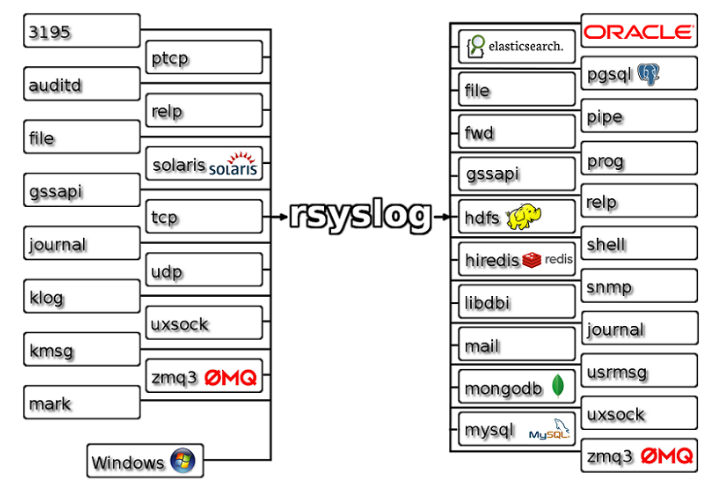
\includegraphics[scale=0.5]{diagramas/rsyslog-esquema.png}}\\
  \caption{Esquema de Rsyslog}
\end{figure}

\begin{itemize}
\item Multihilo
\item TCP, SSL, TLS RELP
\item Se puede filtrar cualquier parte de los mensajes de syslog
\item Se puede configurar el formato de salida de la recolección
\end{itemize}

\subsection{Logrotate}
\label{subsection:logrotate}

Web: \url{https://github.com/logrotate/logrotate}\\
man: \url{http://linux.die.net/man/8/logrotate}\\

Es una utilidad de los sistemas UNIX que nos permite simplificar la administración de archivos de logs en un sistema en dónde haya logs de muchos tipos de fuentes. Nos permite automatizar la rotación, compresión, eliminación y envío por email de los archivos de logs del sistema. Logrotate se encuentra normalmente corriendo cómo un proceso cron diario. \\

\begin{figure}[H]
\begin{lstlisting}[language=bash]
/var/log/iptables.log
        {
                rotate 7
                daily
                missingok
                notifempty
                delaycompress
                compress
                postrotate
                        invoke-rc.d rsyslog restart > /dev/null
                endscript
        }
\end{lstlisting}
\caption{Configuración de iptables para Logrotate}
\end{figure}

Ahora se realizará una breve explicación de cada configuración que se ha establecido sobre el archivo iptables.log:

\begin{itemize}
\item \textbf{rotate <count>}: Los archivos de log son rotados una cantidad de <count> veces antes de ser eliminados o enviados por correo. Si <count> es 0, las versiones anteriores son eliminados antes de efectuarse la rotación.
\item \textbf{daily}: Los archivos de log son rotados diariamente.
\item \textbf{missingok}: Si el archivo de log no existe, ir al siguiente sin mostrar un mensaje de error.
\item \textbf{notifempty}: No rotar el log si éste está vacío.
\item \textbf{delaycompress}: Pospone la compresión de los logs previos para el siguiente ciclo de rotaciones. Esto sólo sucede cuando se combina con la opción \textbf{compress}.
\item \textbf{compress}: Las versiones antiguas de logs son comprimidas con gzip por defecto.
\item \textbf{postrotate-endscript}: Las líneas que se encuentran entre estas dos palabras en la configuración, son ejecutadas (usando /bin/sh) antes de que el archivo de log sea rotado y sólo si el log actual va a ser rotado.

  En este caso, el comando que se ejecuta fuerza a rsyslog a reabrir el archivo de log para escribir en él. Se suele usar después que logrotate mueva los archivos de logs antiguos, entonces rsyslog comienza a escribir en los nuevos.
\end{itemize}

\subsection{Syslog}

Web (man): \url{http://linux.die.net/man/3/syslog}\\

Sirve para el envío de mensajes al sistema de logs interno. syslog() genera un mensaje de log, el cuál se distribuye mediante el demonio syslogd.

\subsection{Iptables}

Web: \url{http://www.netfilter.org/projects/iptables/index.html}\\
Manual: \url{http://www.netfilter.org/documentation/HOWTO/es/packet-filtering-HOWTO-7.html}\\
man: \url{http://linux.die.net/man/8/iptables}\\

Herramienta de filtrado de paquetes IPv4/IPv6 y NAT. Iptables es usado para configurar, mantener e inspeccionar tablas de paquetes IP mediante filtros o reglas en el kernel de Linux. Se pueden definir multitud de tablas, en las que cada una pueda contener un número de reglas precargadas o que pueden ser redefinidas por el usuario. \\

\subsection{Django-rest}

\hspace*{.75in}{
\includegraphics[scale=0.5]{diagramas/django-rest-logo.png}}

Web: \url{http://www.django-rest-framework.org/}\\

Django REST es un framework potente y flexible que permite construir Web APIs. Se usa cómo un complemento al framework Django para el uso de API Restfull dentro de la propia aplicación.

\subsection{JSON}

Web: \url{http://www.json.org/}\\

JSON (Javascript Object Notation) es un formato de intercambio de datos ligero. Se usa para facilitar la legibilidad y escritura para los humanos y además es fácil de interpretar y parsear para una máquina. Está basado cómo un subconjunto de JavaScript y el Standard ECMA-262 3ª Edición. \\

JSON está construido sobre dos estructuras:

\begin{itemize}
\item Una colección de pares nombre/valores. En varios lenguajes, esto se realiza mediante objetos, registros, estructuras, diccionarios, tablas hash, listas de claves o arrays asociativos.
\item Una lista de valores ordenados. En la mayoría de lenguajes, esto se realiza mediante un array, un vector, lista o secuencia.
\end{itemize}

\subsection{PyCharm}

\hspace*{2.25in}{
\includegraphics[scale=0.25]{diagramas/pycharm-logo.png}}

Web: \url{https://www.jetbrains.com/pycharm/}\\

PyCharm es un IDE que permite el trabajo con aplicaciones Python en sus respectivos entornos virtuales (virtualenv) así cómo la integración con frameworks de desarrollo cómo es el caso de Django. La aplicación en sí fue desarrollada nativamente mediante un editor de texto (Emacs) pero a la hora de realizar un empaquetado e integración con otra herramientas se optó por éste IDE. \\

\subsection{Taiga}

\hspace*{2.5in}{
\includegraphics[scale=0.25]{diagramas/taiga-logo.png}}

Web: \url{https://taiga.io/}\\

Taiga es un gestor de proyectos que nos permite implementar una metodología SCRUM o Kanban sobre nuestro proyecto. Es una herramienta muy intuitiva y colaborativa, que permite definir hitos/tareas/wikis para solucionar cada punto de la fase de desarrollo de un proyecto. Además, permite la integración (WebHooks) con otras plataformas de repositorios de proyectos cómo GitHub, GitLab o BitBucket. \\
\newpage
\begin{figure}[H]
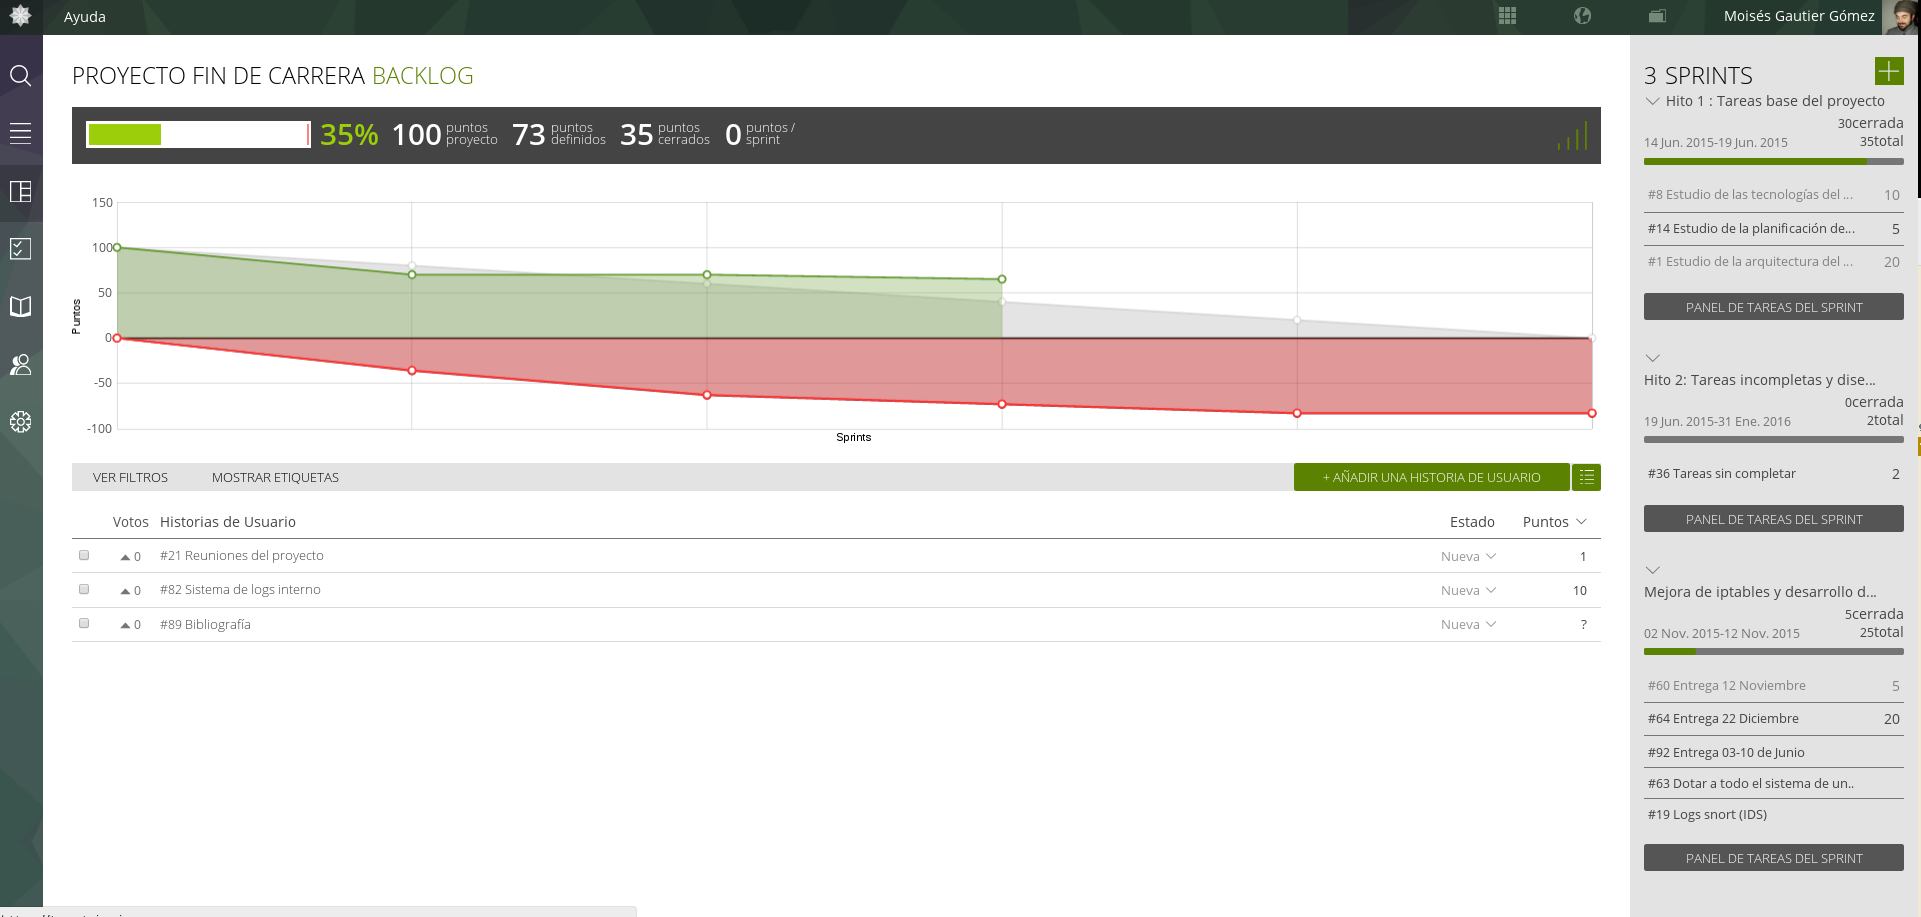
\includegraphics[scale=0.235]{diagramas/taiga-backlog.png}
\caption{Backlog del proyecto siguiendo un SCRUM}
\end{figure}

\subsection{Bitbucket}

\hspace*{2in}{
\includegraphics{diagramas/bitbucket-logo.png}}\\

Web: \url{https://bitbucket.org/}\\
Repositorio: \url{https://bitbucket.org/MGautierGomez/securityproject}\\

Gestor de repositorios Git y Mercurial. Se optó por éste gestor para probar su funcionamiento, así cómo la posibilidad de tener repositorios privados para desarrollar partes del proyecto que necesitasen ser ocultadas. También se encuentra alojado en el repositorio de \textbf{GitHub}: \url{https://github.com/MGautier/security-sensor}\\

\subsection{Git}

\hspace*{2.1in}{
\includegraphics[scale=0.5]{diagramas/git-logo.png}}

Web: \url{https://git-scm.com/}\\

Git es un sistema open-source de control de versiones diseñado para manejar integramente las fases de desarrollo de proyectos, simples y complejos, con velocidad y eficiencia.\\

\subsection{Digital Ocean}

\begin{center}
\includegraphics[scale=0.35]{diagramas/docean-logo.png}\end{center}

Web: \url{https://www.digitalocean.com/}\\

Servidor web para alojar proyectos en cloud. La ventaja de este servicio de VPS es que te permite desplegar máquinas de cualquier tipo (siempre que sean software libre) de una manera muy fácil y rápida. Además tiene un punto fuerte y es que la información se almacena en discos SSD, con lo que el procesamiento se ve muy mejorado a la hora de computar (en este caso eventos de Iptables).\\

\begin{figure}[H]
\hspace*{-1.5in}{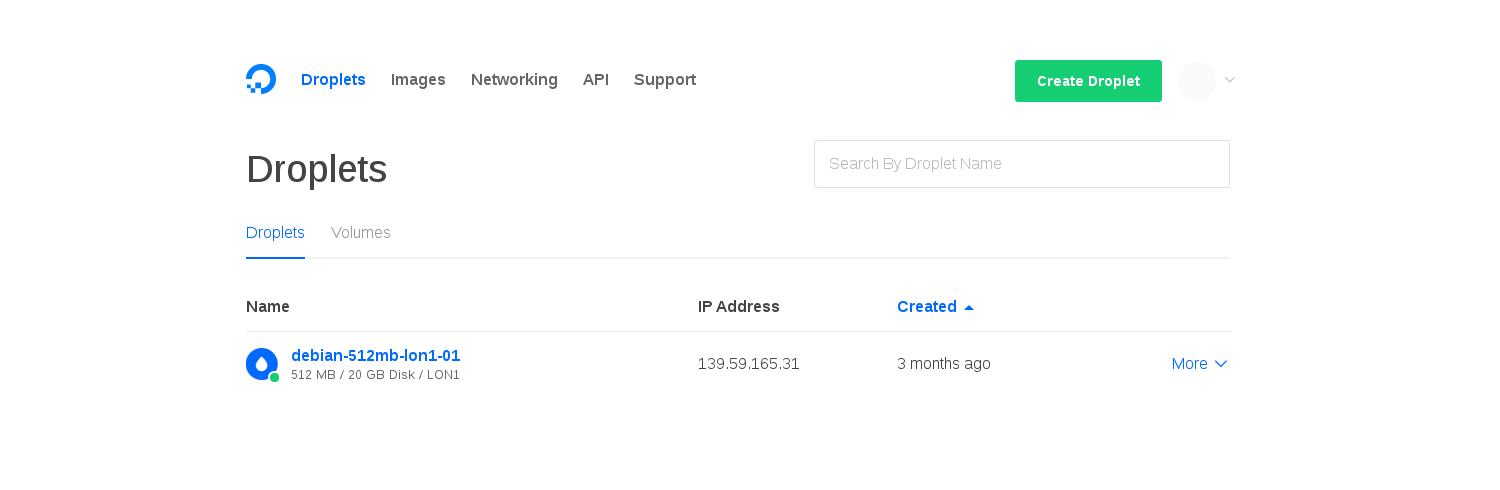
\includegraphics[scale=0.45]{diagramas/droplets.png}}
\caption{Droplet desplegado en digital ocean}
\end{figure}

\subsection{Nginx}

\hspace*{2in}{
\includegraphics[scale=0.5]{diagramas/nginx-logo.png}\\}

Web: \url{http://nginx.org/}\\
Características: \url{http://nginx.org/en/}\\

Nginx (engine x) es un servidor HTTP y proxy inverso, un servidor proxy de email y un servidor proxy genérico de TCP/UDP. Algunas de sus principales características son las siguientes:\\

\begin{itemize}
\item Sirve archivos estáticos, index y autoindexados.
\item Acelera el proceso de proxy inverso con caché: Tolerancia a fallos y carga balanceada de datos.
\item Soporta aceleración con cacheo de FastCGI, uwsgi, SCGI y servidores memcached: Tolerancia a fallos y carga balanceada de datos.
\item Soporta SSL y TLS SNI.
\item Soporta HTTP/2 con dependencia basada en prioridad y balanceo.
\end{itemize}

Configuración de nginx para el servidor en digital ocean:

\begin{figure}[H]
\begin{lstlisting}[language=bash]
server {

        root /var/www/html;

        # Tipos de archivos index de nuestro sistema

        index index.html index.htm index.nginx-debian.html;

        # Nombre del servidor en local

        server_name 139.59.165.31;

        location /static/ {
                alias ~/trunk/version-1-0/webapp/secproject/static/;
                expires 30d;
        }

        location / {
                proxy_set_header X-Forwarded-For $proxy_add_x_forwarded_for;
                proxy_set_header Host $http_host;
                proxy_redirect off;
                proxy_pass http://127.0.0.1:8000;
                proxy_pass_header Server;
                proxy_set_header X-Real-IP $remote_addr;
                proxy_connect_timeout 10;
                proxy_read_timeout 10;


        }
}
\end{lstlisting}
\caption{Configuración de nginx en digital ocean}
\end{figure}

\subsection{Dependencias Python}

Estas son las dependencias que se necesitan para la fase de desarrollo del proyecto. Para poder hacer uso de ellas, previamente tendremos que tener instalado un entorno virtual o virtualenv desde el cual hacer la instalación de estos paquetes.

\subsubsection{Virtualenv}

Es una herramienta que nos permite crear entornos aislados de Python. De esta forma podemos realizar pruebas de dependencias o paquetes para un entorno de desarrollo, en dónde las instalaciones o pruebas no afecten a las dependencias internas del sistema.\\

\begin{itemize}
  \item Django 1.9.2: \url{https://pypi.python.org/pypi/Django/1.9.2}
  \item argparse 1.4.0: \url{https://docs.python.org/2.7/library/argparse.html}
  \item dnspython 1.12.0: \url{https://pypi.python.org/pypi/dnspython/1.12.0} - Se usa para hacer resolución directa e inversa de DNS.
  \item gunicorn 19.4.5: \url{https://pypi.python.org/pypi/gunicorn} - Sirve para desplegar un servidor WSGI (Web Server Gateway Interface) HTTP en entornos Unix.
  \item optional-django 0.3.0: \url{https://pypi.python.org/pypi/optional-django/} - Otras utilidades del framework Django
  \item pygtail 0.6.1: \url{https://pypi.python.org/pypi/pygtail} - Sirve para leer archivos de log en los cuales haya registros del mismo sin leer. Similar al comando tail -f en sistemas Unix.
  \item python-dateutil 2.4.2: \url{https://pypi.python.org/pypi/python-dateutil/2.4.2} - Extensión al módulo principal de Python datetime.
  \item react 2.0.2: \url{https://pypi.python.org/pypi/react/2.0.2} - Módulo que ejecuta un servidor de datos para los componentes react de la aplicación en Python.
  \item requests 2.9.1: \url{https://pypi.python.org/pypi/requests/} - Bibloteca Python para poder consumir recursos HTTP de forma segura y controlada.
  \item setuptools 20.1.1: \url{https://pypi.python.org/pypi/setuptools} - Herramienta para la descarga, compilación, instalación, desinstalación y actualización de todos los paquetes Python. El resultado de la misma se puede usar mediante pip que se nutre el repositorio de paquetes PyPi.
  \item six 1.10.0: \url{https://pypi.python.org/pypi/six} - Es una bibloteca de compatibilidad entre Python 2 y 3.
  \item wheel 0.29.0: \url{https://pypi.python.org/pypi/wheel} - Es un gestor o generador de paquetes en Python.
  \item wsgiref 0.1.2: \url{https://pypi.python.org/pypi/wsgiref} - Es una biblioteca que sirve cómo soporte de validación para WSGI 1.0.1 para versiones de Python inferiores a la 3.2.
  \item configparser 3.5.0: \url{https://docs.python.org/2/library/configparser.html} - Es módulo o clase que implementa un lenguaje muy sencillo para el parseo de archivos de configuración, siguiendo una estructura similar a cómo se describen y procesan los archivos INI en sistemas Microsoft Windows.
\end{itemize}


\chapter[Requisitos]{Especificación y análisis de requisitos}
\label{chap:requisitos}

Los requisitos funcionales y especificación de los mismos son los que a continuación se decriben.

Actualmente existen muchas tecnologías de monitorización de redes que a su vez tiene formato hardware, cómo controladores de sesiones de navegación de usuarios, firewall, proxys que enrutan el tráfico de una compañía hacia las redes externas, autenticación en sistemas VPN para acceso seguro sobre máquinas remotas, etc. El principal problema de estas tecnologías es que cada una pertenece a un ámbito distinto dentro del mismo departamento, es decir, pertenecen a las redes y a tráfico o flujo de comunicaciones pero se enmarcan en diferentes aspectos de cada uno de estos. \\

Para el caso que nos concierte en el proyecto, dentro del marco de investigación que define la totalidad de la infraestructura, la funcionalidad principal del mismo será:

\begin{itemize}
\item Definir los pasos para obtener recolección de logs de una fuente de seguridad. Configuración de rsyslog, logrotate y supervisord (este último en el caso de que sea necesario).
\item Una vez configurada la máquina, configurar la instalación para cada fuente en particular. El ámbito del proyecto se enfoca sobre iptables.
\item Realizar un sistema de parseo de logs para extraer la información necesaria para cada evento que se registre en el sistema.
\item Extracción de características de dichos eventos y procesamiento mediante un algoritmo de frecuencias para detectar las anomalías más comunes.
\item Sistema de gestión de base de datos en dónde se encuentren los datos en crudo recogidos, los procesados y los dispuestos para su visualización.
\item Panel de control dónde visualizar la información de ese nodo con total detalle de la información.
\item Compresión y envio de los datos a la capa superior dónde se alojará el SIEM.
\end{itemize}

\section[Configuración local]{Configuración local para procesamiento}
Los primeros pasos la la obtención de logs o eventos generados por la fuente de seguridad, iptables, serán los de configurar al sistema interno de correlación de logs rsyslog junto con el sistema de rotacion de logs logrotate. Para el caso de rsyslog tenemos que definir un filtro para que cualquier evento que genere el sistema con un determinado mensaje definido en las reglas de iptables, sea capturado y almacenado en un determinado directorio. También hemos dotado a los logs del sistema de timestamp con mayor precisión para poder diferenciar eventos con mayor afinamiento y cambiado la tupla de permisos a la hora de crear un archivo con \textbf{FileCreateMode}.

\begin{figure}[H]
  \begin{lstlisting}[language=bash]
    #
    # Use traditional timestamp format.
    # To enable high precision timestamps, comment out the following line.
    #
    #$ActionFileDefaultTemplate RSYSLOG_TraditionalFileFormat

    #
    # Set the default permissions for all log files.
    #
    $FileOwner root
    $FileGroup adm
    $FileCreateMode 0644
    $DirCreateMode 0755
    $Umask 0022

    # IPTABLES

    :msg,contains,"IPTMSG= " -/var/log/iptables.log
    :msg,regex,"^\[ *[0-9]*\.[0-9]*\] IPTMSG= " -/var/log/iptables.log
    :msg,contains,"IPTMSG= " ~

  \end{lstlisting}
  \caption{Configuración de iptables para Rsyslog}
\end{figure}
\pagebreak
También hemos de configurar Logrotate (más información sobre los campos visitar sección \ref{subsection:logrotate}):

\begin{figure}[H]
\begin{lstlisting}[language=bash]
/var/log/iptables.log
        {
                rotate 7
                daily
                missingok
                notifempty
                delaycompress
                compress
                postrotate
                        invoke-rc.d rsyslog restart > /dev/null
                endscript
        }
\end{lstlisting}
\caption{Configuración de iptables para Logrotate}
\end{figure}

Además tenemos que definir una regla específica para el demonio de rsyslog en la cual se filtre también por los campos que queramos de iptables:

\begin{figure}[H]
\begin{lstlisting}[language=bash]
# into separate file and stop their further processing
if  ($syslogfacility-text == 'kern') and \\
($msg contains 'IPTMSG=' and $msg contains 'IN=') \\
then    -/var/log/iptables.log
    &   ~

\end{lstlisting}
\caption{Configuración de iptables.conf para Rsyslog.d}
\end{figure}

Estos tres paso o configuraciones nos permiten redireccionar un log de iptables al directorio \textbf{/var/log/} y en conreto para el archivo \textbf{iptables.log}. Esta configuración entrará en efecto una vez hayamos reiniciado el servico rsyslog o en el próximo inicio de sesión sobre la máquina.

\pagebreak
\section[Logs]{Recogida y almacenamiento de logs}
Para el caso que nos ocupa, iptables tiene una forma de definir reglas internas para el filtrado de paquetes según el tipo de comunicación que se establezca contra la máquina o desde la máquina hacia el exterior.

\begin{figure}[H]
\begin{lstlisting}[language=bash]
iptables -A INPUT -p tcp -m tcp --dport 22 -j LOG --log-prefix "IPTMSG=Connection SSH "
\end{lstlisting}
\caption{Ejemplo de regla iptables}
\end{figure}

En la siguiente sección explicaremos en profundidad cada una de las opciones de la regla, pero a simple vista podemos observar que el mensaje asociado a la regla coincide con la palabra clave del filtro empleado en rsyslog: \textbf{IPTMSG=}. Así pues, una vez dicho evento se genere el sistema y syslog lo procese como un mensaje de un servicio determinado, en este caso iptables, rsyslog filtrará dicho mensaje según su configuración para almacenarlo posteriormente en \textbf{/var/log/iptables.log}.

\section{Iptables}

El servicio de firewall del kernel de GNU Linux, iptables, nos proporciona una interfaz de reglas y tablas en dónde podemos definir patrones o reglas que actuen sobre el tráfico que llega o sale desde nuestra máquina. Las reglas que se han definido por defecto son las siguientes (si queremos más filtros hay que implicar al protocolo y su puerto asociado con un mensaje):

\begin{figure}[H]
\begin{lstlisting}[language=bash]
# Generated by iptables-save v1.4.21 on Mon Jan 25 20:37:18 2016
*filter
:INPUT ACCEPT [0:0]
:FORWARD ACCEPT [0:0]
:OUTPUT ACCEPT [0:0]
-A INPUT -d 127.0.0.1/32 -p icmp -m icmp --icmp-type 8 -m state --state NEW,RELATED,ESTABLISHED -j LOG --log-prefix "IPTMSG=Connection ICMP "
-A INPUT -d 127.0.0.1/32 -p icmp -m icmp --icmp-type 8 -m state --state NEW,RELATED,ESTABLISHED -j DROP
-A INPUT -p tcp -m tcp --dport 22 -j LOG --log-prefix "IPTMSG=Connection SSH "
-A INPUT -p tcp -m tcp --dport 22 -j DROP
COMMIT
\end{lstlisting}
\caption{Configuracion reglas iptables}
\end{figure}

A continuación una breve explicación de cada opción o comando:
\begin{itemize}
\item -A: Añadir una nueva regla a una cadena de la tabla.
\item -d: Especificación para la ip destino, en este caso localhost con una máscara de subred determinada.
\item --dport: Especificación para el puerto destino al que se realizará la posible conexión o envío de paquetes.
\item -p: Especificación del protocolo del paquete.
\item -m: Especificación de matching, en este caso icmp o tcp dentro de la descripción del paquete.
\item --icmp-type: Extensión del tipo de ping que se va a procesar desde la regla.
\item --state: Tipo de paquete según conexión:
  \begin{itemize}
  \item NEW: Paquete que crea una nueva conexión.
  \item RELATED: Paquete que está relacionado a una conexión existente, pero que no es parte de ella, cómo un error ICMP o, un paquete que establece una conexión de datos FTP.
  \item ESTABLISHED: Paquete que pertenece a una conexión existente (que tuvo paquetes de respuesta).
  \item INVALID (no usado): Paquete que no pudo ser identificado por alguna razón: quedarse sin memoria o errores ICMP que no corresponden a ninguna conexión conocida. Normalmente estos paquetes deben ser descartados.
  \end{itemize}
\item -j: Acción de salto cuando encuentre dicha regla de paquetes. Se especifican dos acciones:
  \begin{itemize}
  \item LOG --log-prefix ``message'' : Cuando se encuentre dicha regla se recolecta cómo log de la misma adjuntando un mensaje para diferenciarla del resto de reglas.
  \item DROP : Cuando se encuentre dicha regla se descarta el paquete dentro del propio sistema. Al ir seguido LOG de un DROP el paquete se muestra en el registro de syslog para posteriormente ser eliminado del registro de almacenamiento de paquetes (Para esto usamos rsyslog que se encarga de almacenar dicho mensaje en un archivo de log).
  \end{itemize}
\end{itemize}

Así pues una vez tengamos un evento o paquete o log de iptables en nuestro sistema generados mediante ssh 127.0.0.1 o ping 127.0.0.1 obtendremos lo siguiente:

\begin{figure}[H]
\begin{lstlisting}[language=bash, breaklines=true]
[dom jul  3 17:04:03 2016] IPTMSG=Connection SSH IN=lo OUT= MAC=00:00:00:00:00:00:00:00:00:00:00:00:08:00 SRC=127.0.0.1 DST=127.0.0.1 LEN=60 TOS=0x00 PREC=0x00 TTL=64 ID=39454 DF PROTO=TCP SPT=47706 DPT=22 WINDOW=43690 RES=0x00 SYN URGP=0
[dom jul  3 17:04:05 2016] IPTMSG=Connection SSH IN=lo OUT= MAC=00:00:00:00:00:00:00:00:00:00:00:00:08:00 SRC=127.0.0.1 DST=127.0.0.1 LEN=60 TOS=0x00 PREC=0x00 TTL=64 ID=39455 DF PROTO=TCP SPT=47706 DPT=22 WINDOW=43690 RES=0x00 SYN URGP=0
\end{lstlisting}
\caption{Evento de ssh localhost en el sistema}
\end{figure}

Lo anterior correspondía a la salida del comando \textbf{\$ dmesg -T} que muestra todos los mensajes del sistema que se han pasado al syslog. La opción -T se usa para especificar el timestamp de cada mensaje con una mayor precisión.\\

\begin{figure}[H]
\begin{lstlisting}[language=bash, breaklines=true]
2016-07-03T17:03:35.664324+02:00 debian kernel: [23337.363387] IPTMSG=Connection SSH IN=lo OUT= MAC=00:00:00:00:00:00:00:00:00:00:00:00:08:00 SRC=127.0.0.1 DST=127.0.0.1 LEN=60 TOS=0x00 PREC=0x00 TTL=64 ID=39454 DF PROTO=TCP SPT=47706 DPT=22 WINDOW=43690 RES=0x00 SYN URGP=0
2016-07-03T17:03:37.668326+02:00 debian kernel: [23339.369692] IPTMSG=Connection SSH IN=lo OUT= MAC=00:00:00:00:00:00:00:00:00:00:00:00:08:00 SRC=127.0.0.1 DST=127.0.0.1 LEN=60 TOS=0x00 PREC=0x00 TTL=64 ID=39455 DF PROTO=TCP SPT=47706 DPT=22 WINDOW=43690 RES=0x00 SYN URGP=0
\end{lstlisting}
\caption{Log capturado y almacenado por rsyslog en /var/log/iptables.log}
\end{figure}

Lo anterior corresponde con la manipulación por parte de rsyslog del mensaje obtenido en syslog. Cómo podemos observar se añade un campo de timestamp de mayor precisión según la configuración que hemos establecido en rsyslog.conf para poder diferenciar con mayor exactitud eventos entre diferentes franjas de tiempo. \\

\begin{figure}[H]
\begin{lstlisting}[language=bash, breaklines=true]
++++++++++++++++++++++++++++++++++++++++++++++++++
--------------------------------------------------

 Procesando linea --> 2016-07-03T17:12:53.632264+02:00 debian kernel: [23896.003739] IPTMSG=Connection ICMP IN=lo OUT= MAC=00:00:00:00:00:00:00:00:00:00:00:00:08:00 SRC=127.0.0.1 DST=127.0.0.1 LEN=84 TOS=0x00 PREC=0x00 TTL=64 ID=64157 DF PROTO=ICMP TYPE=8 CODE=0 ID=14177 SEQ=7

--------------------------------------------------
++++++++++++++++++++++++++++++++++++++++++++++++++
---> Insertado registro: {'TAG': 'Connection ICMP', 'ID_Source_PORT': None, 'Protocol': u'ICMP', 'RAW_Info': '2016-07-03T17:12:53.632264+02:00 debian kernel 23896.003739 IPTMSG=Connection ICMP IN=lo OUT MAC=00:00:00:00:00:00:00:00:00:00:00:00:08:00 SRC=127.0.0.1 DST=127.0.0.1 LEN=84 TOS=0x00 PREC=0x00 TTL=64 ID=64157 DF PROTO=ICMP TYPE=8 CODE=0 ID=14177 SEQ=7 ', 'ID_Source_MAC': <Macs: 00:00:00:00:00:00:00:00:00:00:00:00:08:00>, 'ID_Source_IP': <Ips: 127.0.0.1>, 'ID_Dest_IP': <Ips: 127.0.0.1>, 'ID_Dest_PORT': None, 'ID_Dest_MAC': <Macs: 00:00:00:00:00:00:00:00:00:00:00:00:08:00>}

++++++++++++++++++++++++++++++++++++++++++++++++++
---> Fin de procesado de linea
\end{lstlisting}
\caption{Procesamiento del log capturado y almacenado en la bd interna de la aplicación}
\end{figure}
\pagebreak

\section[Parser]{Transformación de log en información útil: Parser}

Una vez hemos descrito los pasos a seguir para obtener un log para un evento iptables, llega la hora de procesar y hacer útil todos esos datos que tenemos. Para esta finalidad tenemos que usar expresiones regulares para generar un parser con el que ser capaz de traducir todos esos datos en información útil para nuestra aplicación.\\

\begin{figure}[H]
\lstinputlisting{trozos-codigo/codigo-4.py}
\caption{Instancia de la clase Pygtail y lectura de las líneas del log}
\end{figure}

Hacemos uso del módulo o paquete \href{https://pypi.python.org/pypi/pygtail}{Pygtail} que nos permite leer archivos de log que aún no han sido leídos. Es una especie de \textbf{\$ tail -f} a un archivo en concreto, pero usa un concepto de offset e inode para saber la última actualización y posición del archivo antes y después de ser abierto para así saber que parte de la última lectura se quedo en ejecución. Éste es otro punto importante dado que para hacer uso de esta funcionalidad debemos crear un archivo con el nombre del log, véase \textbf{/var/log/iptables.log} cuya extensión final sea offset (\textbf{/var/log/iptables.log.offset}) y sus permisos los siguientes:

\begin{figure}[H]
  \begin{lstlisting}[language=bash, breaklines=true]
    -rw-r--r-- 1 root adm 10391 jul  3 17:12 /var/log/iptables.log
    -rw-r--rw- 1 root root 14 jul  3 17:13 /var/log/iptables.log.offset
  \end{lstlisting}
  \caption{Permisos de los archivos iptables.log e iptables.log.offset}
\end{figure}

Una vez tengamos el archivo abierto y con sus líneas procesadas por Pygtail, es el momento de usar regex sobre los objetos string de cada línea de log. Para ello hacemos uso del método split para dividir por palabras, es decir, posiciones separadas en una lista a todas las coincidencias con una palabra que pudiera tener toda la cadena.\\

\begin{figure}[H]
\lstinputlisting{trozos-codigo/codigo-5.py}
\caption{Uso del método split sobre la entrada de lineas de log}
\end{figure}

Una vez separado por palabras toda la línea de log, pasamos a diferenciar entre las etiquetas que iptables pone a cada campo con su valor, es decir, una tupla key=>value. \\

\begin{figure}[H]
\lstinputlisting{trozos-codigo/codigo-6.py}
\caption{Obtenemos la tupla key=>value para cada etiqueta del log}
\end{figure}

Ya tenemos todas las etiquetas de los campos del log y ahora nos toca extraer su valor asociado para asignarlo al ORM de la base de datos, es decir, almacenar la información en la BD.\\

\begin{figure}[H]
\lstinputlisting{trozos-codigo/codigo-7.py}
\caption{Vamos asignando cada etiqueta y su valor a su asociado del ORM}
\end{figure}

Los siguientes pasos de comprobación de integridad de valores y demás se relegan a la visualización del interesado en el método process\_line del archivo código fuente iptables.py\\

\pagebreak
\section{Workflow}

\section{Extracción de características}

\section{Visualización de eventos}

\section{Compresión}


\chapter{Diseño}
\label{chap:diseño}

A continuación pasaremos a detallar cada una de las partes del diseño del sistema.

\section{Diseño de la arquitectura}

La arquitectura sobre la cual se ha basado el proyecto se representa en el siguiente diagrama correspondiente con una sonda o nodo de recolección de información para el proyecto VERITAS:

\begin{figure}[H]
  \hspace*{0.65in}{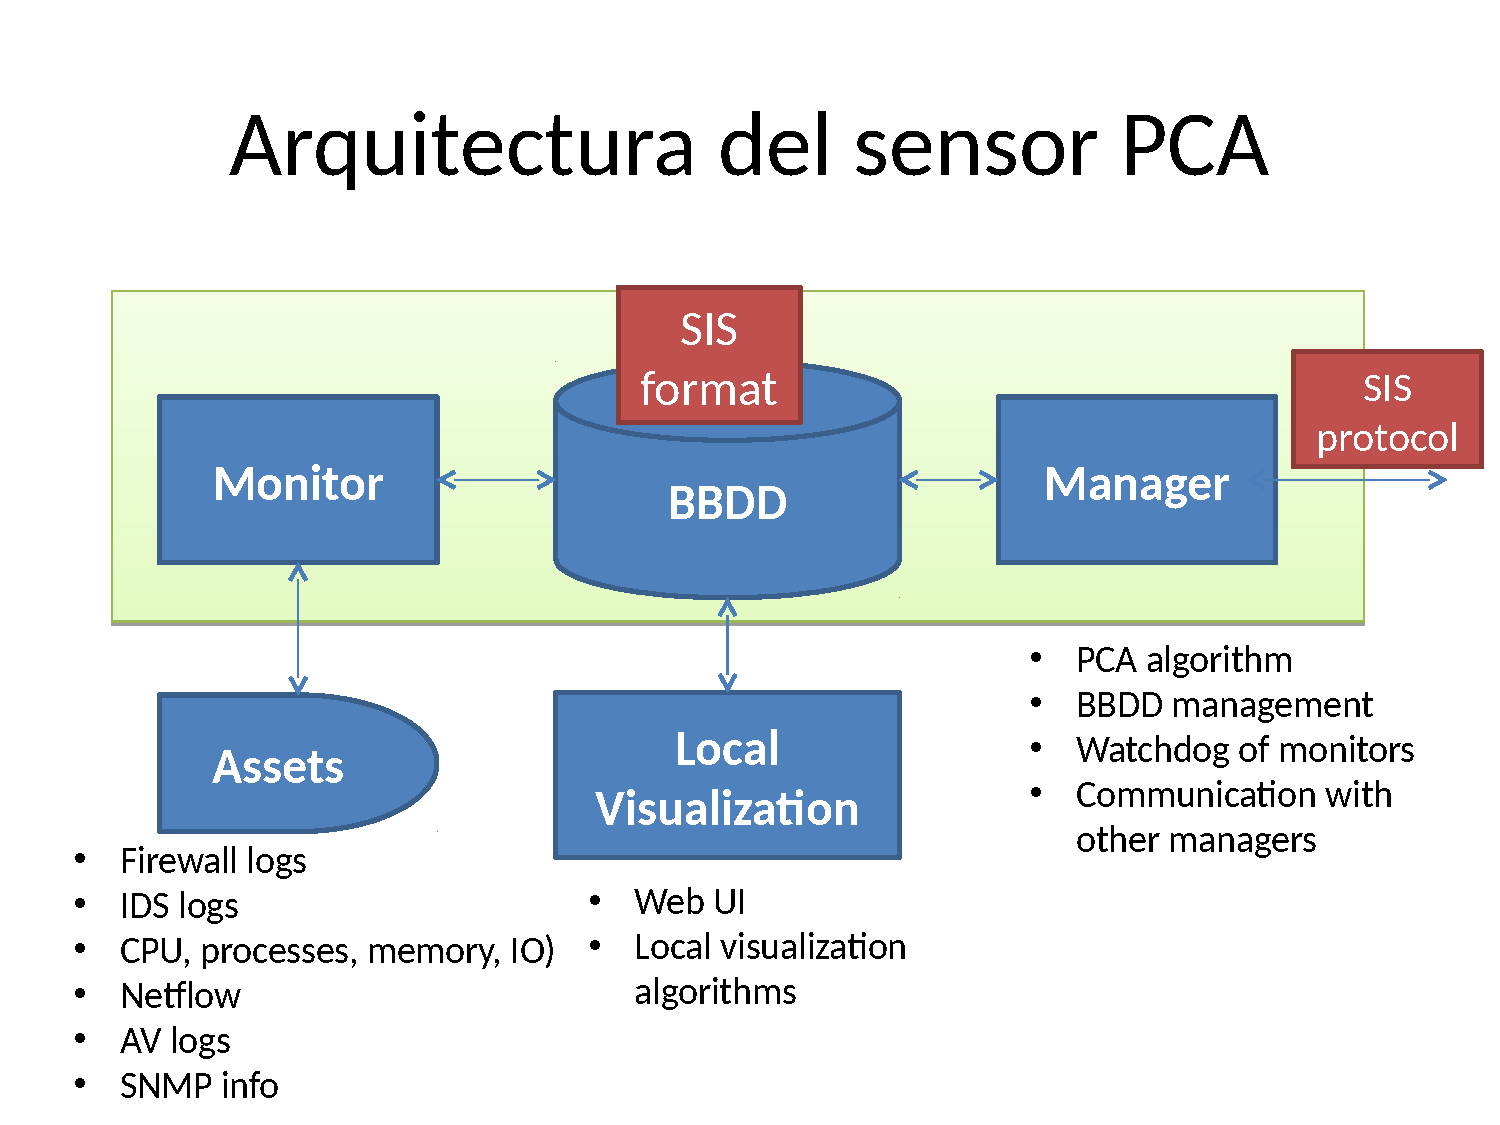
\includegraphics[scale=0.5]{diagramas/Especificaciones.pdf}}
  \caption{Arquitectura interna del software}
\end{figure}

En el esquema podemos ver toda la arquitectura que tendría una sonda para el proyecto VERITAS, aunque el ámbito de éste proyecto no se engloba en su totalidad, sino en unas partes en concreto del esquema que en el siguiente punto se explicarán en detalle. Puntualizar que la interacción de la sonda con la fuente de seguridad es independiente de la interacción base de datos con la visualización de los datos. Si bien se hace uso del mismo ORM, proporcionado por el framework Django, estos se ejecutan por separado a la hora de procesar las fuentes.

\section{Diseño del software de cada módulo}

\subsubsection{Assets}

\begin{figure}[H]
  \hspace*{0.65in}{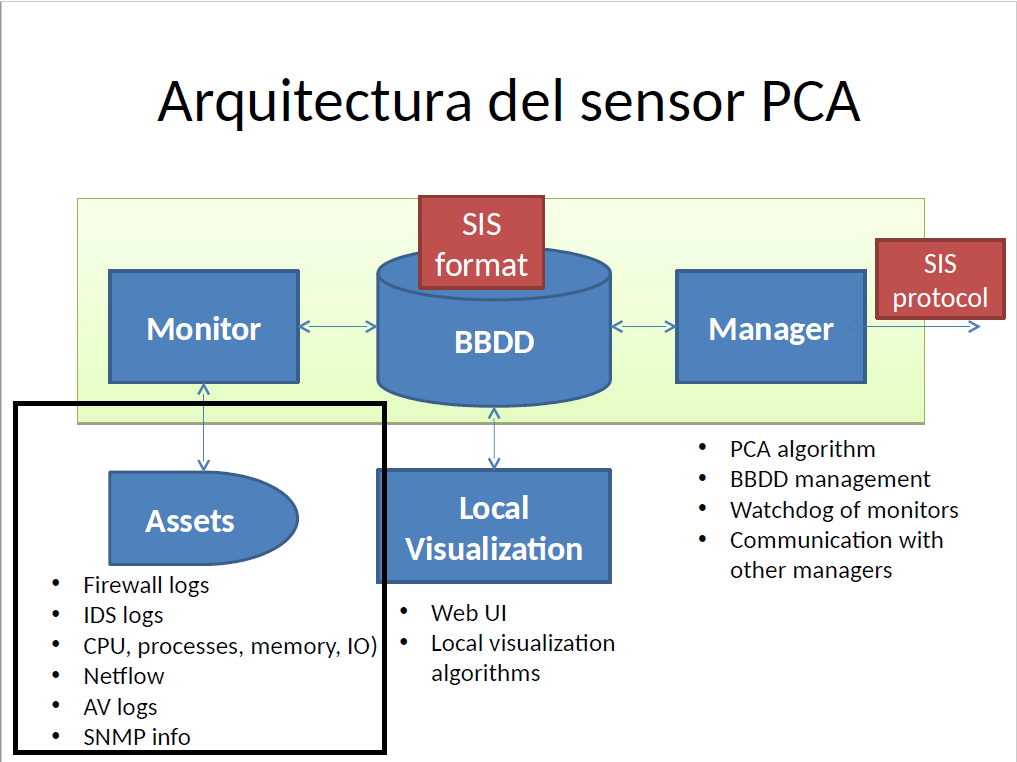
\includegraphics[scale=0.5]{diagramas/assets.png}}
  \caption{Arquitectura: Assets}
\end{figure}

En esta sección de la arquitectura es dónde se define la parte de las fuentes de seguridad que se van a gestionar desde la sonda, es decir, implementar, recolección y pasar el control final a su clase superior: Monitor. La jerarquía de clases sería de la siguiente manera:\\
\newpage
\begin{figure}
  \hspace*{0.05in}{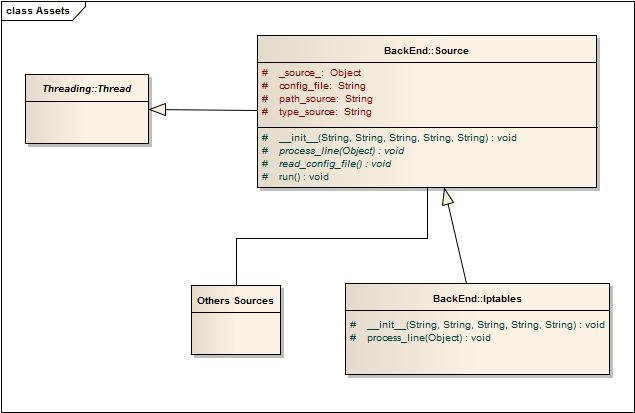
\includegraphics[scale=0.7]{diagramas/diagrama-assets.jpg}}
  \caption{Diagrama de clases: Assets}
\end{figure}

La clase base que sería Source, hereda del comportamiento de la clase Thread (de la biblioteca threading de Python) y a su vez toda fuente de seguridad que se decida implementar heredará de ella los métodos previstos.\\
\newpage

\subsubsection{Monitor}

\begin{figure}[H]
  \hspace*{0.65in}{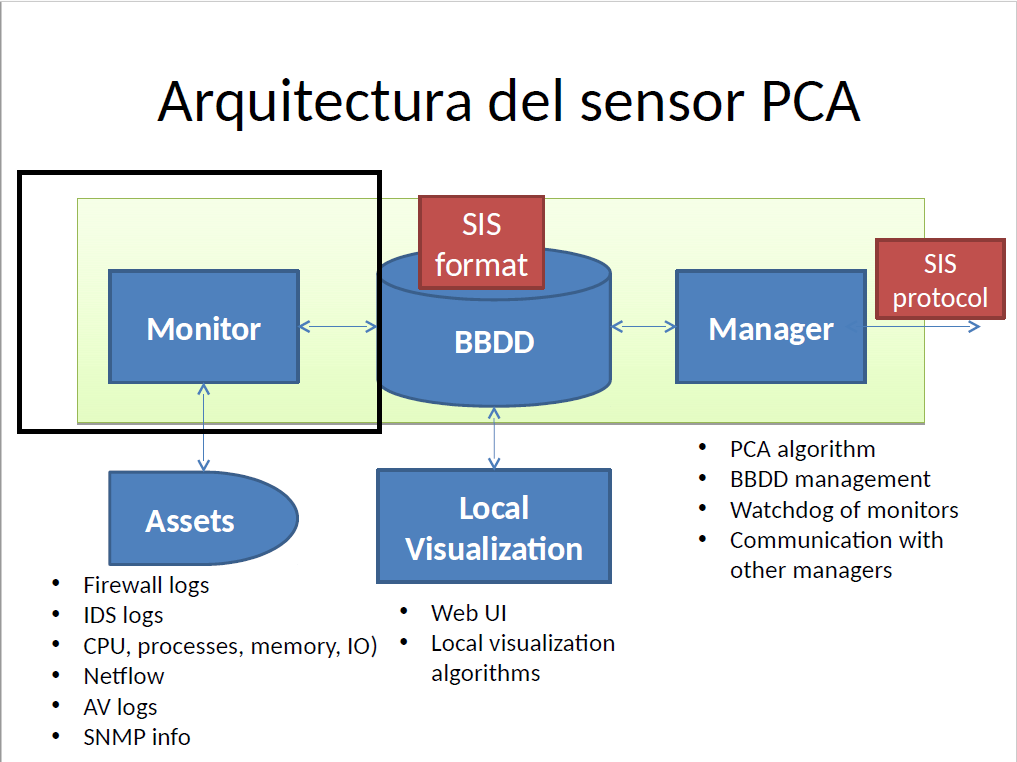
\includegraphics[scale=0.5]{diagramas/monitor.png}}
  \caption{Arquitectura: Monitor}
\end{figure}

En esta sección de la arquitectura es dónde se define la parte del control y ejecución (hilos) de las fuentes de seguridad implementadas. A su vez estas pasan dicha información a la base de datos usando el modelo ORM del framework Django. La jerarquía de clases sería de la siguiente manera: \\

\begin{figure}[H]
  \hspace*{-0.25in}{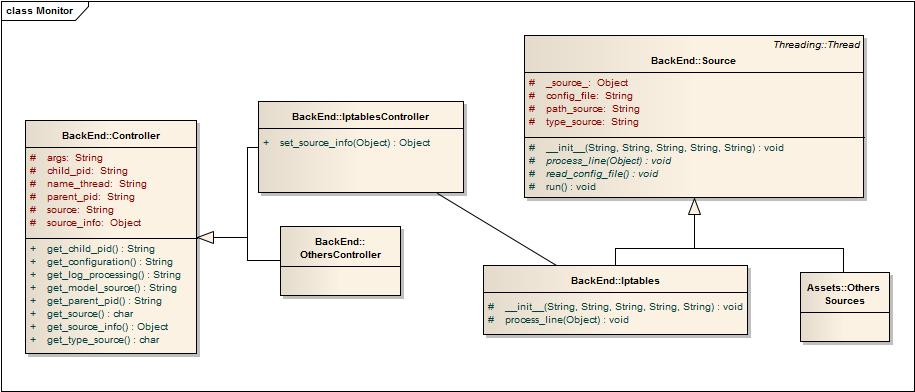
\includegraphics[scale=0.525]{diagramas/diagrama-monitor.jpg}}
  \caption{Diagrama de clases: Assets}
\end{figure}

Nuestra arquitectura monitor se representa con la clase Controller que se encarga de dotar de funcionalidad de ejecución de la fuente (hilo) para unos determinados parámetros de configuración.

\subsubsection{BBDD}

\begin{figure}[H]
  \hspace*{0.65in}{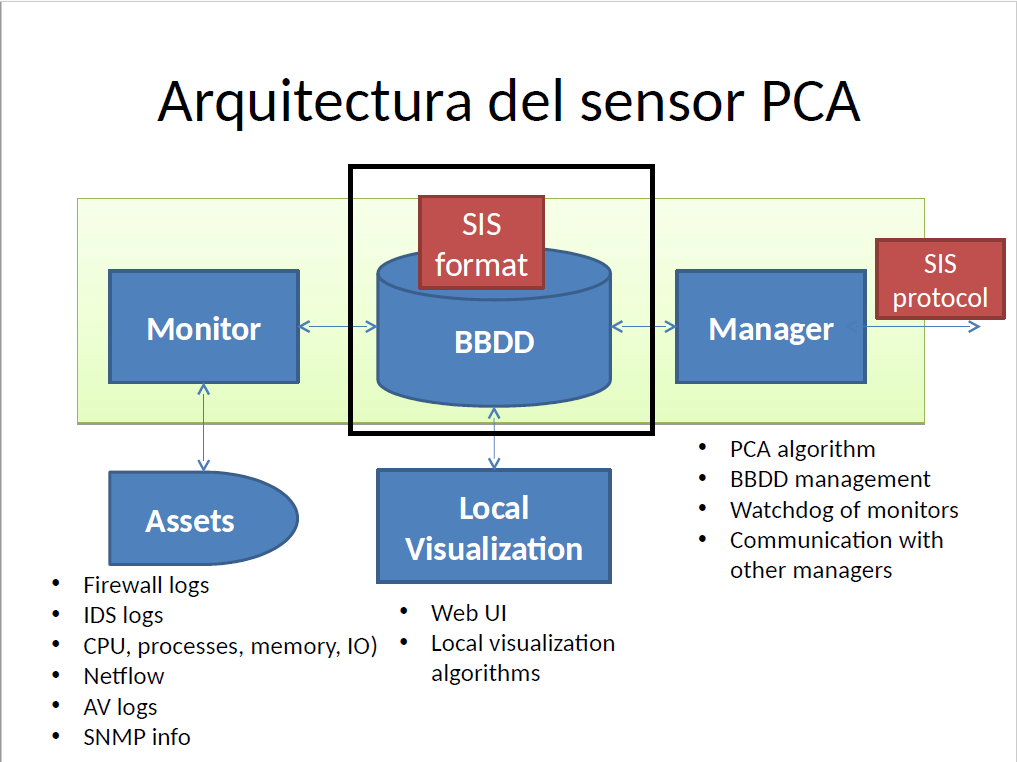
\includegraphics[scale=0.5]{diagramas/bbdd.png}}
  \caption{Arquitectura: Monitor}
\end{figure}

En esta sección de la arquitectura es dónde se define la parte de la interacción con la base de datos y que tablas (clases del modelo ORM) se han definido y con que relaciones. La jerarquía de clases sería de la siguiente manera: \\
\newpage
\begin{figure}[H]
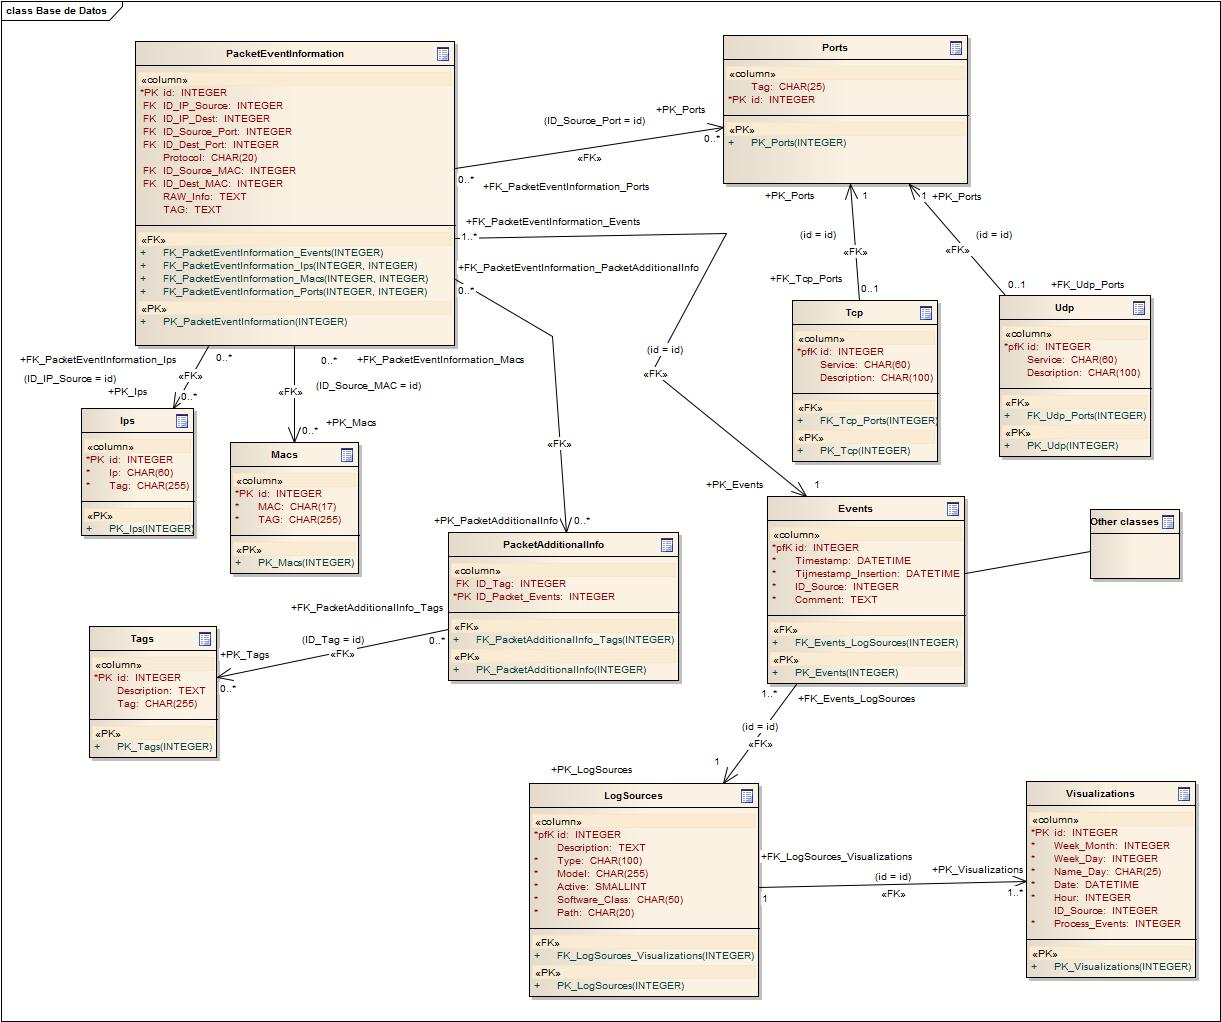
\includegraphics[scale=.35]{diagramas/bd.jpg}
\caption{Diagrama de clases para la BD (usando ORM)}
\end{figure}

La clase o tabla que contendrá el peso de toda la jerarquía de base de datos, será \textbf{PacketEventsInformation}. Esta tabla sólo contendrá referencias externas o ``foreign keys'' a cada tabla que haga participe en su definición, es decir:
\begin{itemize}
\item Ips
\item Macs
\item Ports
\item Events
\item PacketAdditionalInfo
\end{itemize}

Cómo podemos observar en el diagrama anterior, por ejemplo, para la clase PacketEventInformation, tenemos su traducción a formato ORM del motor proporcionado por Django:

\begin{figure}[H]
\lstinputlisting{trozos-codigo/codigo-8.py}
\caption{Ejemplo de clase ORM, en concreto PacketEventsInformation}
\end{figure}

El formato normalizado de la base de datos para visualizar dicha información será mediante JSON, ya que para hacer uso de la información la implementación consumirá dichos datos de la api que se proporciona con la aplicación.\\

\newpage
\subsubsection{Visualizations}

\begin{figure}[H]
  \hspace*{0.65in}{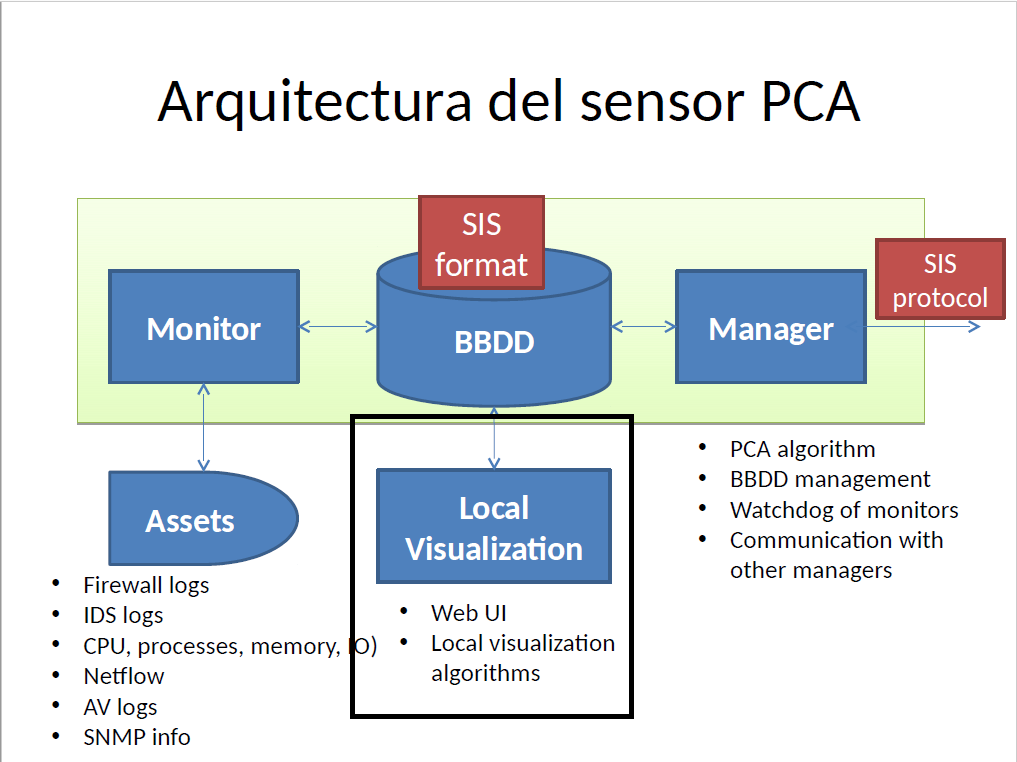
\includegraphics[scale=0.5]{diagramas/visualization.png}}
  \caption{Arquitectura: Visualizaciones}
\end{figure}

En esta seccción de la arquitectura es dónde se define la parte de la interacción con la base de datos y la visualización de los datos en la interfaz web. La jerarquía de clases sería de la siguiente manera: \\

\begin{figure}[H]
  \hspace*{0.5in}{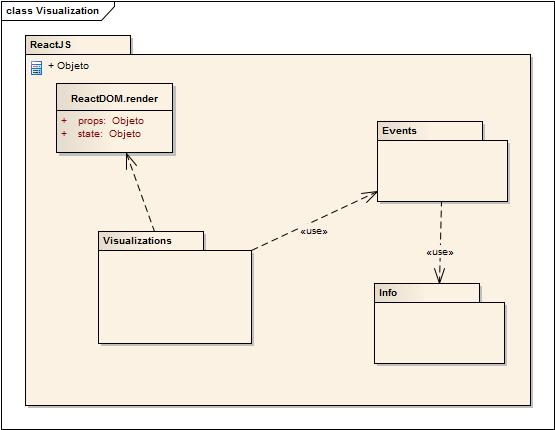
\includegraphics[scale=0.65]{diagramas/visualization.jpg}}
  \caption{Clase Visualization para el paquete ReactJS}
\end{figure}

\begin{figure}[H]
  \hspace*{0.75in}{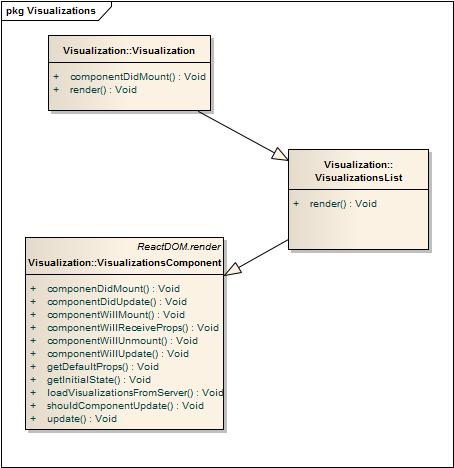
\includegraphics[scale=0.65]{diagramas/visualizations-visualizations.jpg}}
  \caption{Paquete Visualizations}
\end{figure}

\begin{figure}[H]
  \hspace*{0.75in}{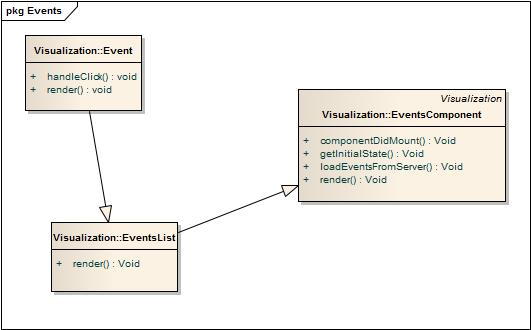
\includegraphics[scale=0.65]{diagramas/visualizations-events.jpg}}
  \caption{Paquete Events}
\end{figure}

\begin{figure}[H]
  \hspace*{2.15in}{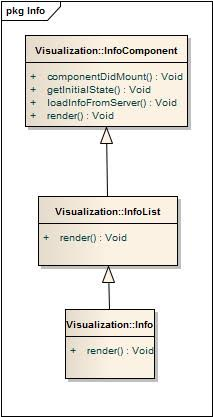
\includegraphics[scale=0.65]{diagramas/visualizations-info.jpg}}
  \caption{Paquete Info}
\end{figure}
\pagebreak
\section{Diagramas de Secuencia - Operaciones}

En esta sección vamos a describir los diagramas de secuencia de operaciones tales como:

\begin{itemize}
\item Ejecución principal de la sonda.
\item Ejecución principal del servidor web que sirve los datos a la interfaz web.
\end{itemize}

Ahora definiremos la parte de diagramas de secuencias para la interacción entre el usuario y el procesamiento de fuentes (Back); y el usuario y la visualización de los datos en la web de la aplicación (Front).\\
\newpage

\subsection{Flujo de ejecución de la aplicación: BackEnd}
\begin{figure}[H]
\vspace*{-.5in}{\hspace*{-.55in}{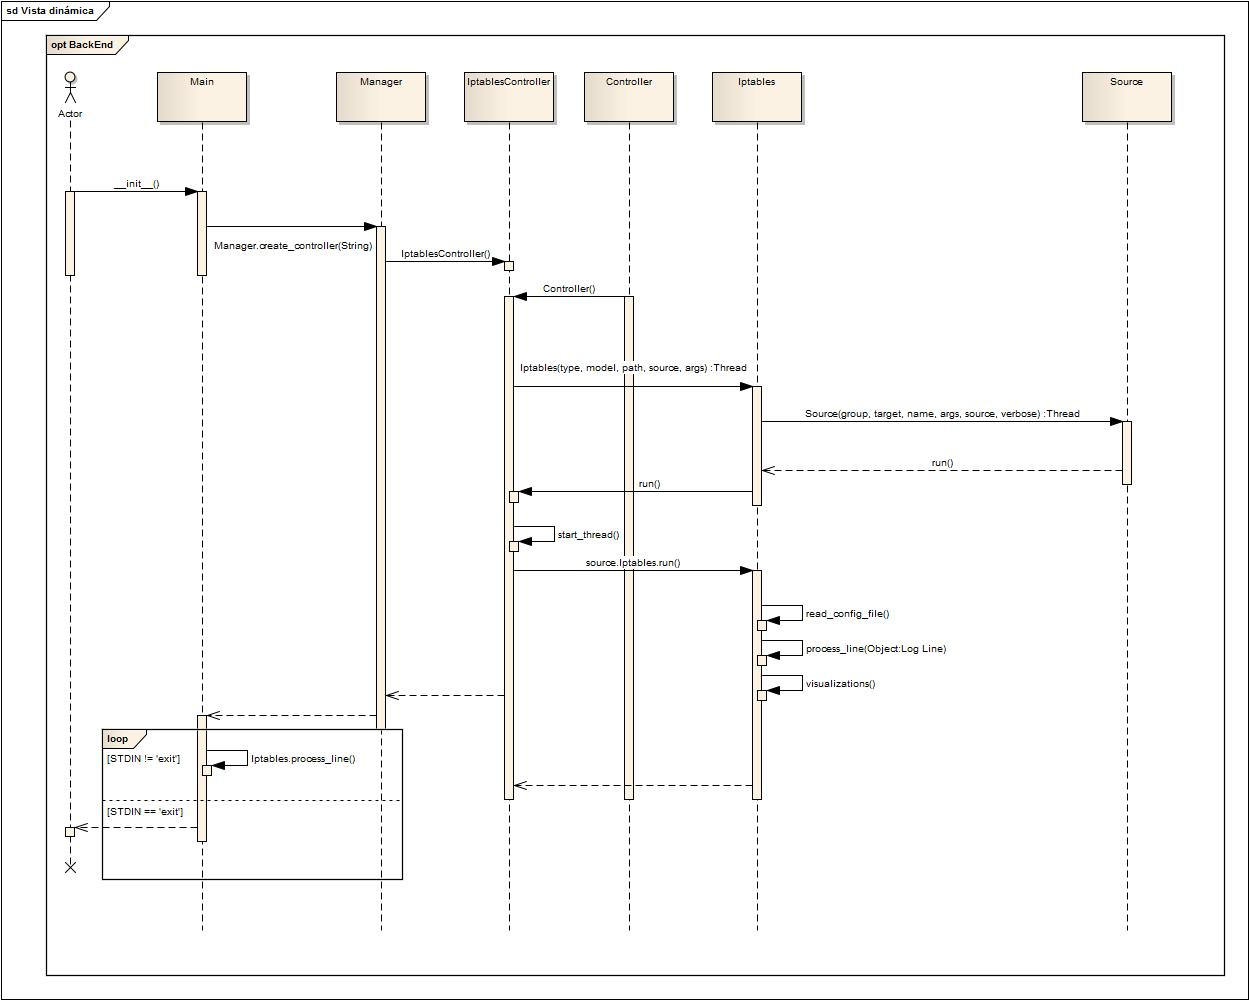
\includegraphics[scale=.5,angle=270]{diagramas/secuencia-back.jpg}}}
\caption{Diagrama de Secuencia para la parte BackEnd}
\end{figure}

\subsection{Flujo de ejecución de la aplicación: FrontEnd}

\begin{figure}[H]
\vspace*{-.1in}{\hspace*{.75in}{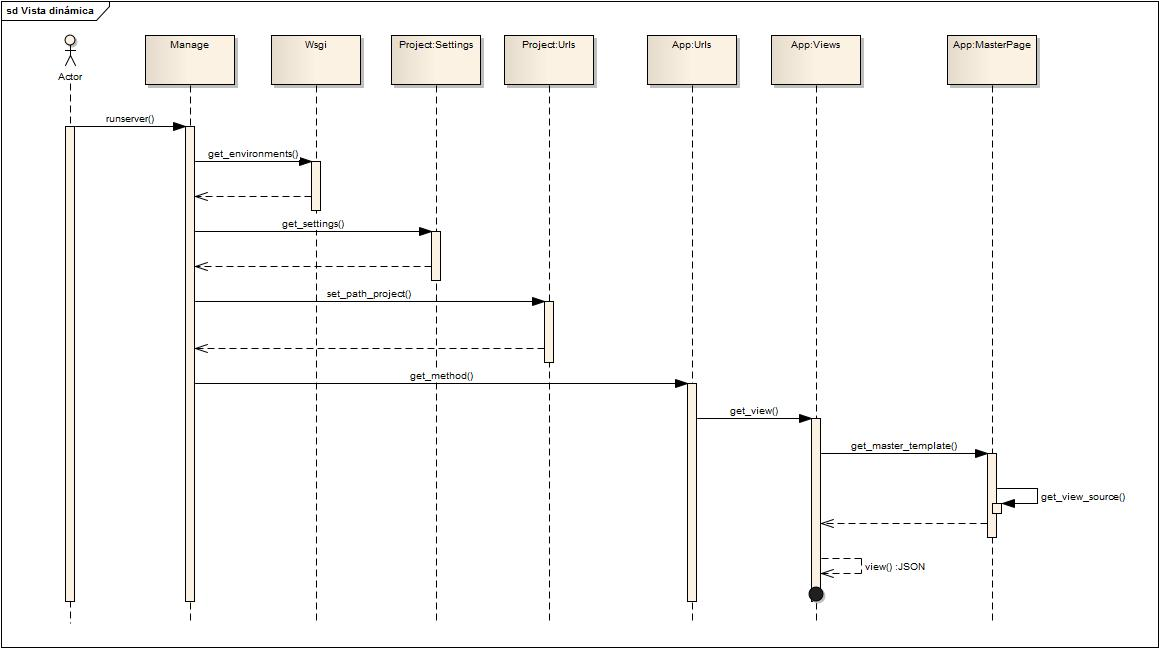
\includegraphics[scale=.5,angle=270]{diagramas/secuencia-front.jpg}}}
\caption{Diagrama de Secuencia para la parte FrontEnd}
\end{figure}

\section{Diseño de la vista}

\subsection{Flujo de interacción de la vista principal}

\begin{figure}[H]
\vspace*{-.1in}{\hspace*{.35in}{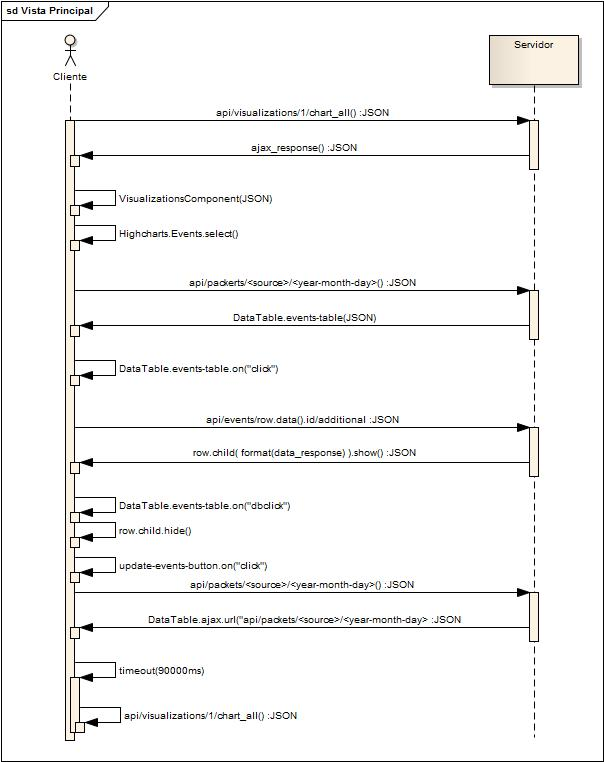
\includegraphics[scale=.7]{diagramas/vista-principal.jpg}}}
\caption{Diagrama de Secuencia para la vista principal}
\end{figure}

\subsection{Flujo de interacción de la vista de eventos en tiempo real}

\begin{figure}[H]
\vspace*{-.1in}{\hspace*{.65in}{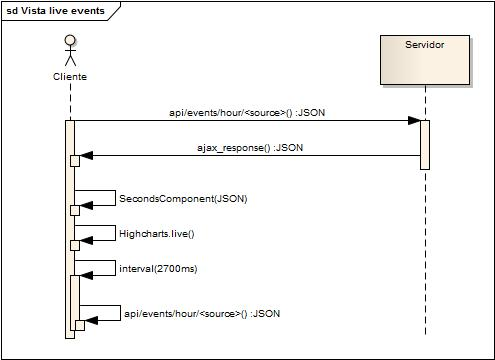
\includegraphics[scale=.7]{diagramas/vista-live-events.jpg}}}
\caption{Diagrama de Secuencia para la vista de eventos en tiempo real}
\end{figure}

\subsection{Flujo de interacción de la vista de estadísticas de los paquetes}

\begin{figure}[H]
\vspace*{-.1in}{\hspace*{.75in}{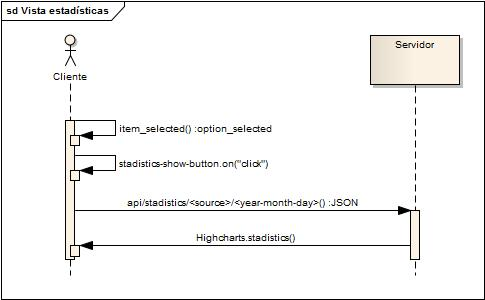
\includegraphics[scale=.7]{diagramas/vista-estadisticas.jpg}}}
\caption{Diagrama de Secuencia para la vista de estadísticas de los paquetes}
\end{figure}

Estos han sido los diagramas de secuencia o interacción que podrá tener la parte de la web con el usuario. Ahora se mostrarán algunas capturas de la parte visual (web) que finalmente se ha obtenido:

\subsubsection{Vista Principal}

\begin{figure}[H]
\vspace*{-.5in}{\hspace*{.55in}{\includegraphics[scale=.32,angle=270]{diagramas/web_2.png}}}
\caption{Vista principal de la Web}
\end{figure}

\subsubsection{Vista con información de los eventos}

\begin{figure}[H]
\vspace*{.2in}{\hspace*{.55in}{\includegraphics[scale=.32,angle=270]{diagramas/web_3.png}}}
\caption{Vista principal con la información de eventos del dia seleccionado}
\end{figure}

\subsubsection{Vista con la información adicional por evento}

\begin{figure}[H]
\vspace*{.2in}{\hspace*{.55in}{\includegraphics[scale=.32,angle=270]{diagramas/web_4.png}}}
\caption{Vista principal con la información adicional por cada evento seleccionado}
\end{figure}

\subsubsection{Vista con las estadísticas del día seleccionado}

\begin{figure}[H]
\vspace*{.2in}{\hspace*{.55in}{\includegraphics[scale=.32,angle=270]{diagramas/web_5.png}}}
\caption{Vista principal con las estadísticas de los eventos del día seleccionado}
\end{figure}


\chapter{Implementación}
\label{chap:implementación}

En este capítulo se definirán las configuraciones, diagramas e implementaciones que se han llevado a cabo en el proyecto. Primero, especificaremos los diagramas de clases para el BackEnd y FrontEnd (Flujo de ejecución Django) de la aplicación.

\section{Flujo de ejecución BackEnd}

\begin{figure}[H]
  \hspace*{-.5in}{\includegraphics[scale=0.5]{diagramas/back-end.jpg}}
  \caption{Diagrama de clases BackEnd}
\end{figure}

En el diagrama podemos ver de izquierda a derecha la herencia que hay entre las clases que se encargan de recoger la información de la sonda.\\

\section{Flujo de ejecución FrontEnd}

\begin{figure}[H]
  \begin{center}
  \includegraphics[scale=0.7]{diagramas/django-workflow.png}
  \caption{Flujo de ejecución del FrontEnd - ~\cite{74}}
  \end{center}
\end{figure}

Para este caso se ha decidido mostrar el flujo de ejecución que sigue una petición desde que llega al servidor de Django hasta que se sirve una vista asociada al navegador. \\

\section{Configuración de la aplicación}

En la fase de implementación del proyecto entran en juego la configuración previa de la máquina en la cuál se van a desplegar los componentes para su utilización. Hay ciertos factores a tener en cuenta. \\

Dado que se ha desarrollado una primera version funcional de la aplicación, en el futuro se podrían incluir ciertas herramientas software de automatización de despliegues y configuraciones como podrían ser:
\pagebreak
\subsection{Chef}
Web: \url{https://www.chef.io/}\\
\begin{figure}[H]
  \begin{center}
    \includegraphics[scale=0.3]{diagramas/chef-logo.png}
  \end{center}
\end{figure}

Chef es una plataforma de automatización de gran alcance que nos transforma el control de infraestructuras en código. Da igual el sistema operativo o plataforma sobre el que se tenga que operar, Chef automatiza configuraciones de infraestructuras, desplegados y gestionado a través de la red, sin importar el tamaño de la solución software a controlar.\\

A continuación un diagrama explicando la arquitectura de un sistema bajo Chef:

\begin{figure}[H]
  \begin{center}
  \includegraphics[scale=1]{diagramas/chef.png}
  \caption{Arquitectura de un sistema bajo Chef}
  \end{center}
\end{figure}

\subsection{Ansible}
Web: \url{https://www.ansible.com/}\\
\begin{figure}[H]
  \begin{center}
    \includegraphics[scale=0.1]{diagramas/ansible-logo.png}
  \end{center}
\end{figure}

Ansible es una herramienta de código abierto que se utiliza para distribuir aplicaciones en nodos o servidores remotos de una manera automatizada. Nos proporciona un framework común a todas las aplicaciones, permitiendo así configurar cada una de ellas de una manera más fácil y eficaz. Ansible se basa en ``playbooks'' (al contrario de Chef que se basa en Cookbooks) dónde se pueden definir una amplia variedad de sistemas para el despliegue de una aplicación.

\begin{figure}[H]
  \begin{center}
  \includegraphics[scale=.5]{diagramas/ansible.jpg}
  \caption{Diagrama de la arquitectura Ansible}
  \end{center}
\end{figure}

\subsection{Docker}
Web: \url{https://www.docker.com/}\\
\begin{figure}[H]
  \begin{center}
    \includegraphics[scale=0.5]{diagramas/docker-logo.png}
  \end{center}
\end{figure}

Docker es un sistema de desarrollo de sistemas completos, utilizando el concepto de contenedor (LXC) de los sistemas UNIX. Un contenedor de Docker, envuelve un fragmento de software en un sistema de archivos completo (imagen) que contiene todo lo necesario para funcionar: código, instancias de arranque, herramientas del sistema, bibliotecas del sistema... cualquier cosa que tendría un sistema operativo normal pero en una versión más optimizada y ligera (estos sistemas normalmente se obtienen de un Docker Repository y en su totalidad son sistemas open source). Esto garantiza que el software se ejecutará siempre de la misma forma, independientemente del medio en el que se despliegue.\\

\begin{figure}[H]
  \hspace*{-.1in}{\includegraphics[scale=0.4]{diagramas/docker.png}}
  \caption{Diagrama de la arquitectura general de Docker}
\end{figure}
\vspace*{-.12in}{
\begin{minipage}{\linewidth}
\section[Configuración local]{Configuración local para procesamiento}
Los primeros pasos para la obtención de logs o eventos generados por la fuente de seguridad, iptables, serán los de configurar el sistema interno de correlación de logs rsyslog junto con el sistema de rotación de logs logrotate. Para el caso de rsyslog tenemos que definir un filtro para que cualquier evento que genere el sistema con un determinado mensaje definido en las reglas de iptables, sea capturado y almacenado en un determinado directorio. También hemos dotado a los logs del sistema de timestamp con mayor precisión para poder diferenciar eventos con mayor afinamiento y cambiado la tupla de permisos a la hora de crear un archivo con \textbf{FileCreateMode}.
\end{minipage}}
\begin{figure}[H]
  \begin{lstlisting}[language=bash]
    #
    # Use traditional timestamp format.
    # To enable high precision timestamps, comment out the following line.
    #
    #$ActionFileDefaultTemplate RSYSLOG_TraditionalFileFormat

    #
    # Set the default permissions for all log files.
    #
    $FileOwner root
    $FileGroup adm
    $FileCreateMode 0644
    $DirCreateMode 0755
    $Umask 0022

    # IPTABLES

    :msg,contains,"IPTMSG= " -/var/log/iptables.log
    :msg,regex,"^\[ *[0-9]*\.[0-9]*\] IPTMSG= " -/var/log/iptables.log
    :msg,contains,"IPTMSG= " ~

  \end{lstlisting}
  \caption{Configuración de iptables para Rsyslog}
\end{figure}
\pagebreak
\begin{minipage}{\linewidth}
Hemos de configurar Logrotate (más información sobre los campos visitar sección \ref{subsection:logrotate}):

\begin{figure}[H]
\begin{lstlisting}[language=bash]
/var/log/iptables.log
        {
                rotate 7
                daily
                missingok
                notifempty
                delaycompress
                compress
                postrotate
                        invoke-rc.d rsyslog restart > /dev/null
                endscript
        }
\end{lstlisting}
\caption{Configuración de iptables para Logrotate}
\end{figure}

Tenemos que definir una regla específica para el demonio de rsyslog en la cual se filtre también por los campos que queramos de iptables:

\begin{figure}[H]
\begin{lstlisting}[language=bash]
# into separate file and stop their further processing
if  ($syslogfacility-text == 'kern') and \\
($msg contains 'IPTMSG=' and $msg contains 'IN=') \\
then    -/var/log/iptables.log
    &   ~

\end{lstlisting}
\caption{Configuración de iptables.conf para Rsyslog.d}
\end{figure}

Estos tres pasos o configuraciones nos permiten redireccionar un log de iptables al directorio \textbf{/var/log/} y en conreto para el archivo \textbf{iptables.log}. Esta configuración tendrá efecto una vez hayamos reiniciado el servico rsyslog o en el próximo inicio de sesión sobre la máquina.

\pagebreak
\subsection[Logs]{Recogida y almacenamiento de logs}
Para el caso que nos ocupa, iptables tiene una forma de definir reglas internas para el filtrado de paquetes según el tipo de comunicación que se establezca contra la máquina o desde la máquina hacia el exterior.

\begin{figure}[H]
\begin{lstlisting}[language=bash]
iptables -A INPUT -p tcp -m tcp --dport 22 -j LOG --log-prefix "IPTMSG=Connection SSH "
\end{lstlisting}
\caption{Ejemplo de regla iptables}
\end{figure}

En la siguiente sección explicaremos en profundidad cada una de las opciones de la regla, pero a simple vista podemos observar que el mensaje asociado a la regla coincide con la palabra clave del filtro empleado en rsyslog: \textbf{IPTMSG=}. Así pues, una vez dicho evento se genere el sistema y syslog lo procese como un mensaje de un servicio determinado, en este caso iptables, rsyslog filtrará dicho mensaje según su configuración para almacenarlo posteriormente en \textbf{/var/log/iptables.log}.
\end{minipage}
\subsection{Iptables}

El servicio de firewall del kernel de GNU Linux, iptables, nos proporciona una interfaz de reglas y tablas en donde podemos definir patrones o reglas que actuen sobre el tráfico que llega o sale desde nuestra máquina. Las reglas que se han definido por defecto son las siguientes (si queremos más filtros hay que implicar al protocolo y su puerto asociado con un mensaje):

\begin{figure}[H]
\begin{lstlisting}[language=bash]
# Generated by iptables-save v1.4.21 on Mon Jan 25 20:37:18 2016
*filter
:INPUT ACCEPT [0:0]
:FORWARD ACCEPT [0:0]
:OUTPUT ACCEPT [0:0]
-A INPUT -d 127.0.0.1/32 -p icmp -m icmp --icmp-type 8 -m state --state NEW,RELATED,ESTABLISHED -j LOG --log-prefix "IPTMSG=Connection ICMP "
-A INPUT -d 127.0.0.1/32 -p icmp -m icmp --icmp-type 8 -m state --state NEW,RELATED,ESTABLISHED -j DROP
-A INPUT -p tcp -m tcp --dport 22 -j LOG --log-prefix "IPTMSG=Connection SSH "
-A INPUT -p tcp -m tcp --dport 22 -j DROP
COMMIT
\end{lstlisting}
\caption{Configuración reglas iptables}
\end{figure}

A continuación una breve explicación de cada opción o comando:
\begin{itemize}
\item -A: Añadir una nueva regla a una cadena de la tabla.
\item -d: Especificación para la ip destino, en este caso localhost con una máscara de subred determinada.
\item --dport: Especificación para el puerto destino al que se realizará la posible conexión o envío de paquetes.
\item -p: Especificación del protocolo del paquete.
\item -m: Especificación de matching, en este caso icmp o tcp dentro de la descripción del paquete.
\item --icmp-type: Extensión del tipo de ping que se va a procesar desde la regla.
\item --state: Tipo de paquete según conexión:
  \begin{itemize}
  \item NEW: Paquete que crea una nueva conexión.
  \item RELATED: Paquete que está relacionado a una conexión existente, pero que no es parte de ella, como un error ICMP o, un paquete que establece una conexión de datos FTP.
  \item ESTABLISHED: Paquete que pertenece a una conexión existente (que tuvo paquetes de respuesta).
  \item INVALID (no usado): Paquete que no pudo ser identificado por alguna razón: quedarse sin memoria o errores ICMP que no corresponden a ninguna conexión conocida. Normalmente estos paquetes deben ser descartados.
  \end{itemize}
\item -j: Acción de salto cuando encuentre dicha regla de paquetes. Se especifican dos acciones:
  \begin{itemize}
  \item LOG --log-prefix ``message'' : Cuando se encuentre dicha regla se recolecta como log de la misma adjuntando un mensaje para diferenciarla del resto de reglas.
  \item DROP : Cuando se encuentre dicha regla se descarta el paquete dentro del propio sistema. Al ir seguido LOG de un DROP el paquete se muestra en el registro de syslog para posteriormente ser eliminado del registro de almacenamiento de paquetes (Para esto usamos rsyslog que se encarga de almacenar dicho mensaje en un archivo de log).
  \end{itemize}
\end{itemize}

Así pues, una vez tengamos un evento o paquete o log de iptables en nuestro sistema generados mediante ssh 127.0.0.1 o ping 127.0.0.1 obtendremos lo siguiente:

\begin{figure}[H]
\begin{lstlisting}[language=bash, breaklines=true]
[dom jul  3 17:04:03 2016] IPTMSG=Connection SSH IN=lo OUT= MAC=00:00:00:00:00:00:00:00:00:00:00:00:08:00 SRC=127.0.0.1 DST=127.0.0.1 LEN=60 TOS=0x00 PREC=0x00 TTL=64 ID=39454 DF PROTO=TCP SPT=47706 DPT=22 WINDOW=43690 RES=0x00 SYN URGP=0
[dom jul  3 17:04:05 2016] IPTMSG=Connection SSH IN=lo OUT= MAC=00:00:00:00:00:00:00:00:00:00:00:00:08:00 SRC=127.0.0.1 DST=127.0.0.1 LEN=60 TOS=0x00 PREC=0x00 TTL=64 ID=39455 DF PROTO=TCP SPT=47706 DPT=22 WINDOW=43690 RES=0x00 SYN URGP=0
\end{lstlisting}
\caption{Evento de ssh localhost en el sistema}
\end{figure}

Lo anterior correspondía a la salida del comando \textbf{\$ dmesg -T} que muestra todos los mensajes del sistema que se han pasado al syslog. La opción -T se usa para especificar el timestamp de cada mensaje con una mayor precisión.\\

\begin{figure}[H]
\begin{lstlisting}[language=bash, breaklines=true]
2016-07-03T17:03:35.664324+02:00 debian kernel: [23337.363387] IPTMSG=Connection SSH IN=lo OUT= MAC=00:00:00:00:00:00:00:00:00:00:00:00:08:00 SRC=127.0.0.1 DST=127.0.0.1 LEN=60 TOS=0x00 PREC=0x00 TTL=64 ID=39454 DF PROTO=TCP SPT=47706 DPT=22 WINDOW=43690 RES=0x00 SYN URGP=0
2016-07-03T17:03:37.668326+02:00 debian kernel: [23339.369692] IPTMSG=Connection SSH IN=lo OUT= MAC=00:00:00:00:00:00:00:00:00:00:00:00:08:00 SRC=127.0.0.1 DST=127.0.0.1 LEN=60 TOS=0x00 PREC=0x00 TTL=64 ID=39455 DF PROTO=TCP SPT=47706 DPT=22 WINDOW=43690 RES=0x00 SYN URGP=0
\end{lstlisting}
\caption{Log capturado y almacenado por rsyslog en /var/log/iptables.log}
\end{figure}

Lo anterior corresponde con la manipulación por parte de rsyslog del mensaje obtenido en syslog. Como podemos observar se añade un campo de timestamp de mayor precisión según la configuración que hemos establecido en rsyslog.conf para poder diferenciar con mayor exactitud eventos entre diferentes franjas de tiempo. \\

\begin{figure}[H]
\begin{lstlisting}[language=bash, breaklines=true]
++++++++++++++++++++++++++++++++++++++++++++++++++
--------------------------------------------------

 Procesando linea --> 2016-07-03T17:12:53.632264+02:00 debian kernel: [23896.003739] IPTMSG=Connection ICMP IN=lo OUT= MAC=00:00:00:00:00:00:00:00:00:00:00:00:08:00 SRC=127.0.0.1 DST=127.0.0.1 LEN=84 TOS=0x00 PREC=0x00 TTL=64 ID=64157 DF PROTO=ICMP TYPE=8 CODE=0 ID=14177 SEQ=7

--------------------------------------------------
++++++++++++++++++++++++++++++++++++++++++++++++++
---> Insertado registro: {'TAG': 'Connection ICMP', 'ID_Source_PORT': None, 'Protocol': u'ICMP', 'RAW_Info': '2016-07-03T17:12:53.632264+02:00 debian kernel 23896.003739 IPTMSG=Connection ICMP IN=lo OUT MAC=00:00:00:00:00:00:00:00:00:00:00:00:08:00 SRC=127.0.0.1 DST=127.0.0.1 LEN=84 TOS=0x00 PREC=0x00 TTL=64 ID=64157 DF PROTO=ICMP TYPE=8 CODE=0 ID=14177 SEQ=7 ', 'ID_Source_MAC': <Macs: 00:00:00:00:00:00:00:00:00:00:00:00:08:00>, 'ID_Source_IP': <Ips: 127.0.0.1>, 'ID_Dest_IP': <Ips: 127.0.0.1>, 'ID_Dest_PORT': None, 'ID_Dest_MAC': <Macs: 00:00:00:00:00:00:00:00:00:00:00:00:08:00>}

++++++++++++++++++++++++++++++++++++++++++++++++++
---> Fin de procesado de linea
\end{lstlisting}
\caption{Procesamiento del log capturado y almacenado en la bd interna de la aplicación}
\end{figure}

\subsection[Parser]{Transformación de log en información útil: Parser}

Una vez hemos descrito los pasos a seguir para obtener un log para un evento iptables, llega la hora de procesar y hacer útil todos esos datos que tenemos. Para esta finalidad tenemos que usar expresiones regulares para generar un parser con el que ser capaz de traducir todos esos datos en información útil para nuestra aplicación.\\

\begin{figure}[H]
\lstinputlisting{trozos-codigo/codigo-4.py}
\caption{Instancia de la clase Pygtail y lectura de las líneas del log}
\end{figure}

Hacemos uso del módulo o paquete \href{https://pypi.python.org/pypi/pygtail}{Pygtail} que nos permite leer archivos de log cuyos registros internos aún no han sido leídos. Es una especie de \textbf{\$ tail -f} a un archivo en concreto, pero usa un concepto de offset e inode para saber la última actualización y posición del archivo antes y después de ser abierto para así saber que parte de la última lectura se quedo en ejecución. Éste es otro punto importante dado que para hacer uso de esta funcionalidad debemos crear un archivo con el nombre del log, véase \textbf{/var/log/iptables.log} cuya extensión final sea offset (\textbf{/var/log/iptables.log.offset}) y sus permisos los siguientes:\\
\vspace*{-.5in}{
\begin{minipage}{\linewidth}
\begin{figure}[H]
  \begin{lstlisting}[language=bash, breaklines=true]
    -rw-r--r-- 1 root adm 10391 jul  3 17:12 /var/log/iptables.log
    -rw-r--rw- 1 root root 14 jul  3 17:13 /var/log/iptables.log.offset
  \end{lstlisting}
  \caption{Permisos de los archivos iptables.log e iptables.log.offset}
\end{figure}

Una vez tengamos el archivo abierto y con sus líneas procesadas por Pygtail, es el momento de usar regex sobre los objetos string de cada línea de log. Para ello hacemos uso del método split para dividir por palabras, es decir, posiciones separadas en una lista a todas las coincidencias con una palabra que pudiera tener toda la cadena.\\

\begin{figure}[H]
\lstinputlisting{trozos-codigo/codigo-5.py}
\caption{Uso del método split sobre la entrada de lineas de log}
\end{figure}

Una vez separado por palabras toda la línea de log, pasamos a diferenciar entre las etiquetas que iptables pone a cada campo con su valor, es decir, una tupla key=>value. \\

\begin{figure}[H]
\lstinputlisting{trozos-codigo/codigo-6.py}
\caption{Obtenemos la tupla key=>value para cada etiqueta del log}
\end{figure}

Ya tenemos todas las etiquetas de los campos del log y ahora nos toca extraer su valor asociado para asignarlo al ORM de la base de datos, es decir, almacenar la información en la BD.
\end{minipage}}
\begin{minipage}{\linewidth}
\begin{figure}[H]
\lstinputlisting{trozos-codigo/codigo-7.py}
\caption{Vamos asignando cada etiqueta y su valor a su asociado del ORM}
\end{figure}

Los siguientes pasos de comprobación de integridad de valores y demás se relegan a la visualización del interesado en el método process\_line del archivo código fuente iptables.py\\
\end{minipage}

\subsection{Workflow}
Ahora vamos a detallar los pasos que seguirá la aplicación a la hora de la visualización de información en la web mediante el framework Django. Pero primero cómo se procesan y almacenan los datos de los logs:\\

\begin{itemize}
\item Primera instancia a ejecutar main.py: Se definen las llamadas al sistema Manager que se encargará a su vez de llamar al controlador que se asocia con la fuente encargada (iptables).
\item Segunda instancia a ejecutar manager.py: Gestión de los controladores que hacen uso de la herramienta. Cada controlador tendrá asociada su fuente.
\item Tercera instancia a ejecutar controller.py: Esta clase contiene unas características que herederán los controladores de cada fuente y a su vez lanza la ejecución de los hilos para cada una de las fuentes. Aquí se define o exporta la variable de entorno de Django para utilizar el ORM del mismo.
\item Cuarta instancia a ejecutar source.py: Aunque se vaya directamente al siguiente punto, primero se pasa el control a esta clase de la cuál hereda iptables y se crean los fragmentos de código para la ejecución en iptables.
\item Quinta instancia a ejecutar iptables.py: Ejecución y configuración de todo el entramado de iptables, de la insercción de datos en la BD y de la extracción de características de los logs.
\end{itemize}

Ahora corresponde el turno al flujo de ejecución para la visualización web:\\

\begin{itemize}
\item Primera instancia a ejecutar manage.py: Aquí se cargan las configuraciones por defecto del proyecto Django para la aplicación definida.
\item Segunda instancia a ejecutar wsgi.py: Se usa la biblioteca wsgi para poder lanzar la aplicación por su nombre dentro del namespace definido por Django.
\item Tercera instancia a ejecutar settings.py: Se cargan todas las configuraciones establecidas por el usuario para el proyecto y que a su vez usarán cómo configuración base para las aplicaciones derivadas del mismo.
\item Cuarta instancia a ejecutar urls.py (archivo que pertenece al proyecto Django): Aquí se encamina la visualización entre la aplicación o la parte de administración del proyecto.
\item Quinta instancia a ejecutar urls.py (archivo que pertenece a la aplicación): Aquí es dónde se define el router de la aplicación web y los métodos que se lanzarán una vez se hagan las peticiones sobre el servidor web Django.
\item Sexta instancia a ejecutar views.py: Se ejecuta el método asociado a la renderización de la vista, que por defecto, sino hay ninguna ruta será index. Dependiendo del método a ejecutar sólo mostrará contenido estático o dinámico (JSON) obtenido de la base de datos.
\item Séptima instancia a ejecutar aplicacion/index.html (Paso previo de MasterPage.html): Se carga el trozo de esta plantilla o template (que en nuestro caso es una vista) que contiene el esqueleto principal de la parte web para todas las vistas/plantillas que heredan de esta general.
\item Octava instancia a ejecutar aplicacion/index.html (Carga de la plantilla index.html): Se carga el trozo de esta plantilla dentro del bloque definido en la plantilla MasterPage que anteriormente se proceso.
\end{itemize}


\subsection{Visualización de eventos}

Aquí tenemos una vista general de todas las interacciones posibles con la web de los eventos almacenados en el sistema.
\newpage
\begin{figure}[H]
\vspace*{.2in}{\hspace*{.55in}{\includegraphics[scale=.33,angle=270]{diagramas/web_8.png}}}
\caption{Vista general}
\end{figure}


\chapter{Evaluación}
\label{chap:evaluación}

\begin{itemize}
\item pruebas funcionales y no funcionales
\item caja blanca
\item caja negra
\end{itemize}


\chapter{Planificación y estimación de costes}
\label{chap:planificacion}

Ya tengo hecho así por encima el diagrama de gantt de todo el proyecto. Tendría que definir las tareas en el diagrama pero lo que haré será meter aquí los apuntes que he ido metiendo en la herramienta Taiga para que se vea alguna descripción o apuntes que he ido tomando por cada tarea del diagrama.


\section{Software utilizado}

El lenguaje usado es python 2.7, luego django con todo los paquetes asociados (poner algún enlace de referencia dónde se listen los paquetes más importantes que he tenido que instalar sin nombrar todas las dependencias de estas)

He usado cómo IDE Pycharm del projecto jetbrains

Para la memoria \LaTeX y para las gráficas tikz supongo.

\section{Licencia}

La licencia del proyecto para su posterior uso. En el actual repositorio de bitbucket no se ha especificado la licencia tal cuál, pero cuando ya este más estable el asunto también lo pondre en github para subirlo y demás. Ahí ya si que tendré que especificarla. En principio sino es para ningún propositio comercial, con la MIT sería suficiente. Sino alguna variante de la GPL o la Mozilla o similares.




\chapter{Conclusiones}
\label{chap:conclusiones}

Durante la realización de éste proyecto, se han conseguido los siguientes resultados:

\begin{itemize}
\item Comprender el funcionamiento de los servicios del sistema: rsyslog, syslog, logrotate, nginx.
\item Comprender el funcionamiento del firewall del kernel, Iptables.
\item Desarrollar una solución software usando el lenguaje de programación Python.
\item Desarrollar una solución software, para sistemas web, usando el framework Django.
\item Manipulación de bases de datos relacionales usando un modelo orientado a objetos (ORM) proporcionado por el framework de desarrollo.
\item Diseñar el prototipo base para los sensores de recopilación de información de seguridad.
\item Diseñar una interfaz web dónde el usuario pueda visualizar la información que el sensor ha analizado.
\item Despliegue de la aplicación en un servidor web en la nube para realizar demostraciones de la herramienta (Digital Ocean).
\item Documentar todo el proceso de realización del proyecto.
\end{itemize}
\pagebreak
A partir de los resultados obtenidos durante la realización de éste proyecto se han extraído las siguientes conclusiones:

\begin{itemize}
\item La aplicación \textit{Sensor para recopilación y visualización de información de seguridad en nodos de una red} es una herramienta que permite el análisis de información de dispositivos de seguridad para una máquina en una red.
\item El código fuente implementado, responde a los objetivos que debe cumplir el desarrollo del proyecto.
\item Con el diseño de la interfaz web se ha conseguido que un usuario sin conocimientos sobre el sistema sea capaz de entender lo que se está registrando en él y que tipo de información de seguridad puede disponer a la hora de realizar un estudio de la misma.
\end{itemize}


\chapter{Apéndice 1: Instalación}
\label{chap:instalacion}

\section{Instalación de Django y VirtualEnv}

Primero tenemos que instalarnos un entorno virtual de desarrollo para que nuestra aplicación no modifique nuestros paths internos de Python, o si bien queremos que todo lo que nos instalemos sea de uso general no tendríamos que hacer este paso. Para ello vamos a la página oficial del proyecto \href{https://virtualenv.pypa.io/en/stable/installation/}{virtualenv} y seguimos los puntos de instalación que nos indican.\\

Una vez configurado e instalado el paquete VirtualEnv en nuestra máquina, pasamos a utilizarlo dentro de nuestro proyecto base. Para ello simplemente, una vez clonado el mismo, vamos a la ruta ``trunk/version-1-0/webapp/'' y ejecutamos lo siguiente:\\

\begin{figure}[H]
  \begin{lstlisting}[language=bash]
    $ virtualenv .
    $ . bin/activate
  \end{lstlisting}
  \caption{Configuración de nuestro entorno virtual de Python}
\end{figure}

Una vez dispuesto nuestro entorno virtual vamos a instalar las dependencias necesarias para el funcionamiento de la aplicación. [Para este paso es necesario tener instalado el paquete \href{https://pip.pypa.io/en/stable/installing/}{pip}, que es el gestor de paquetes del lenguaje Python]\\

\begin{figure}[H]
  \begin{lstlisting}[language=bash]
    $ pip install -U pip
    $ pip install -r requirements.txt
  \end{lstlisting}
  \caption{Instalación de las dependencias del proyecto}
\end{figure}

Ahora es el momento de configurar nuestro proyecto Django para su ejecución:

\begin{figure}[H]
  \begin{lstlisting}[language=bash]
    $ cd secproject
    $ ./manage.py makemigrations
    $ ./manage.py migrate
    $ ./manage.py createsuperuser #Esto nos crea el superuser de administracion
  \end{lstlisting}
  \caption{Configuracion de la base de datos y creacion del super usuario}
\end{figure}

Si queremos especificar un usuario distinto a uno general para diferenciar entre entornos de desarrollo y producción, tendremos que acceder a la dirección ``http://127.0.0.1:8000/admin'', ingresar con el super usuario y definir nuevos usuarios para nuestra aplicación. Para nuestro propósito se ha definido un usuario llamado ``pfc'' para la parte de desarrollo de la aplicación. Una vez finalizada, se podrá establecer para un usuario normal o para otro específico.\\

\section{Rsyslog}

Ya tenemos configurado nuestro entorno de desarrollo de Django, ahora tenemos que configurar los servicios internos de la máquina para que correlen la información generada por iptables en nuestro caso. Así pues, vamos a configurar rsyslog para que redirija los eventos de iptables a ``/var/log/iptables.log''.\\

Incluímos las siguientes líneas en el archivo ``/etc/rsyslog.conf'':

\begin{figure}[H]
  \begin{lstlisting}[language=bash]
    # IPTABLES

    :msg,contains,"IPTMSG= " -/var/log/iptables.log
    :msg,regex,"^[ [0-9].[0-9]*] IPTMSG= " -/var/log/iptables.log
    :msg,contains,"IPTMSG= " ~
  \end{lstlisting}
  \caption{Configuración para filtrado de eventos de Iptables}
\end{figure}

Damos la tupla de permisos 0644 a la creación de archivos:

\begin{figure}[H]
  \begin{lstlisting}[language=bash]
   $ FileCreateMode 0644
  \end{lstlisting}
  \caption{Permisos a la creación de archivos}
\end{figure}

Para obtener timestamps más precisos tenemos que comentar la siguiente línea dentro del archivo de configuración de rsyslog:

\begin{figure}[H]
  \begin{lstlisting}[language=bash]
    #$ActionFileDefaultTemplate RSYSLOG_TraditionalFileFormat
  \end{lstlisting}
  \caption{Timestamp más preciso}
\end{figure}

\section{LogRotate}

Ahora tenemos que configurar el servicio LogRotate para que una vez finalizado el día, los archivos de logs antiguos, los comprima y los almacene en ``/var/log/''. Para ello vamos a la ruta ``/etc/logrotate.d/'' y creamos el archivo ``iptables'' con el siguiente contenido:

\begin{figure}[H]
  \begin{lstlisting}[language=bash]
    /var/log/iptables.log
    {
      rotate 7
      daily
      missingok
      notifempty
      delaycompress
      compress
      postrotate
      invoke-rc.d rsyslog restart > /dev/null
      endscript
    }
  \end{lstlisting}
  \caption{Configuración de LogRotate}
\end{figure}

\section{/var/log/iptables.log}

Tenemos que crear un archivo llamado ``iptables.log'' en ``/var/log'' con las siguientes características:

\begin{figure}[H]
  \begin{lstlisting}[language=bash]
    -rw-r--r-- 1 root adm 15604061 oct 26 20:28 /var/log/iptables.log
    $ chmod 644
    $ chown root:admin
  \end{lstlisting}
  \caption{Creación del archivo base de iptables.log}
\end{figure}

\section{Offset paquete PygTail}

El paquete PygTail usa para la lectura de logs dentro de nuestro sistema un archivo ``.offset'' del que consultará información relacionada del archivo del cual queremos obtener el texto correspondiente. Como por defecto, éste no puede ejecutarse con privilegios de super usuario dentro de la ruta ``/var/log'' o hacemos que nuestra aplicación corra directamente sobre super usuario (opción desaconsejada) o creamos el siguiente archivo para cada log que queramos procesar mediante PygTail.

\begin{figure}[H]
  \begin{lstlisting}[language=bash]
    -rw-r--rw- 1 root root    13 may  9 20:24 /var/log/iptables.log.offset
    $ chmod 646
    $ chown root:root
  \end{lstlisting}
  \caption{Creación del archivo offset de PygTail}
\end{figure}

\section{Rsyslog.d}

Tenemos que decirle al demonio de Rsyslog que todo lo que contenga el mensaje ``IPTMSG'' (que será nuestro mensaje prefijo para cada paquete obtenido mediante Iptables) lo mande a ``/var/log/itpables.log''. Para ello vamos a ``/etc/rsyslog.d/iptables.conf'' e introducimos lo siguiente:

\begin{figure}[H]
  \begin{lstlisting}[language=bash]
    # into separate file and stop their further processing
    if  ($syslogfacility-text == 'kern') and \\
    ($msg contains 'IPTMSG=' and $msg contains 'IN=') \\
    then    -/var/log/iptables.log
        &   ~
  \end{lstlisting}
  \caption{Creación del archivo de configuración iptables para el demonio Rsyslog}
\end{figure}

\section{Iptables}

Los pasos anteriores es para la recolección de eventos generados por Iptables dentro de nuestra máquina. Obviamente habrá que definir unas reglas de filtrado en Iptables cuyo campo de mensaje contenga la siguiente clave/prefijo ``IPTMSG= '' (incluir un espacio al final del mensaje). Aquí un ejemplo de las reglas que se han usado para la generación de eventos Iptables:

\begin{figure}[H]
  \begin{lstlisting}[language=bash]
    # Generated by iptables-save v1.4.21 on Mon Jan 25 20:37:18 2016
    *filter
    :INPUT ACCEPT [0:0]
    :FORWARD ACCEPT [0:0]
    :OUTPUT ACCEPT [0:0]
    -A INPUT -d 127.0.0.1/32 -p icmp -m icmp --icmp-type 8 -m state --state NEW,RELATED,ESTABLISHED -j LOG --log-prefix "IPTMSG=Connection ICMP "
    -A INPUT -d 127.0.0.1/32 -p icmp -m icmp --icmp-type 8 -m state --state NEW,RELATED,ESTABLISHED -j DROP
    -A INPUT -p tcp -m tcp --dport 22 -j LOG --log-prefix "IPTMSG=Connection SSH "
    -A INPUT -p tcp -m tcp --dport 22 -j DROP
    COMMIT
  \end{lstlisting}
  \caption{Reglas de Iptables usadas para el proyecto}
\end{figure}

\section{Web Server}

Ahora ya sólo nos queda configurar nuestro servidor web, que en este caso será Nginx. \textbf{Importante:} Previamente no debe haberse instalado una versión de servidor web Apache, sino habrá que desinstalar todo y aún así dará muchos problemas. Por lo que es altamente recomendable que la instalación este limpia del paquete apache en cualquiera de sus versiones.

\subsection{Nginx}

Instalación de Nginx:

\begin{figure}[H]
  \begin{lstlisting}[language=bash]
    $ sudo apt-get install nginx
  \end{lstlisting}
  \caption{Instalación del paquete Nginx}
\end{figure}

Configuración de Nginx:
\begin{itemize}
\item Vamos a la carpeta ``/etc/nginx/sites-available/'' y creamos nuestro archivo de configuración ``myproject.conf'' con el siguiente contenido:

  \begin{figure}[H]
    \begin{lstlisting}[language=bash]
      server {

        root /var/www/html;

        # Tipos de archivos index de nuestro sistema

        index index.html index.htm index.nginx-debian.html;

        # Nombre del servidor en local

        server_name localhost;

        location /static/ {
          alias <ruta-descarga-proyecto>/securityproject/trunk/ \\
                 version-1-0/webapp/secproject/secapp/static/;
          expires 30d;
        }

        location / {
          proxy_set_header X-Forwarded-For $proxy_add_x_forwarded_for;
          proxy_set_header Host $http_host;
          proxy_redirect off;
          proxy_pass http://127.0.0.1:8000;
          proxy_pass_header Server;
          proxy_set_header X-Real-IP $remote_addr;
          proxy_connect_timeout 10;
          proxy_read_timeout 10;


        }
      }
    \end{lstlisting}
    \caption{Configuración del servidor web en Nginx}
  \end{figure}
\item Una vez hemos escrito el archivo de configuración hacemos un enlace simbólico del mismo a otra carpeta de nginx, en este caso a ``sites-enabled/''
  \begin{figure}[H]
    \begin{lstlisting}[language=bash]
      $ sudo ln -s /etc/nginx/sites-available/myproject.conf /etc/nginx/sites-enabled/
    \end{lstlisting}
    \caption{Enlace simbólico a nuestra configuración previa}
  \end{figure}
\item Para comprobar que los archivos de configuración no tienen errores, ejecutamos el siguiente comando y si es éxito, reiniciamos el servicio:
  \begin{figure}[H]
    \begin{lstlisting}[language=bash]
      $ sudo nginx -t
      $ sudo service nginx restart
    \end{lstlisting}
    \caption{Comprobación de sintaxis de Nginx}
  \end{figure}
\item Ahora nos vamos al proyecto Django y lanzamos la instancia:
  \begin{figure}[H]
    \begin{lstlisting}[language=bash]
      $ ./manage.py runserver
    \end{lstlisting}
    \caption{Ejecución del servidor de Django}
  \end{figure}
\end{itemize}

Si la configuración se ha realizado correctamente, los contenidos estáticos de la web se verán en el navegador y no tendremos que entrar por el puerto 8000 sino por la dirección de loopback directamente: \href{http://127.0.0.1/secapp}{http://127.0.0.1/secapp} ó \href{http://127.0.0.1/admin}{http://127.0.0.1/admin}


\chapter{Apéndice 2: Tests}
\label{chap:tests}

En éste apéndice se tratarán en profundidad el resto de test realizados a las clases del modelo relacional de la base de datos del sistema.

\section{\quad Ips}

\lstinputlisting{trozos-codigo/codigo-9-ips-class.py}

\subsection{\quad Método: test\_ips}

\lstinputlisting{trozos-codigo/codigo-9-ips-test-ips.py}

\subsection{\quad Método: test\_ips\_hostname}

\lstinputlisting{trozos-codigo/codigo-9-ips-test-ips-hostname.py}

\subsection{\quad Método: test\_ips\_tag}

\lstinputlisting{trozos-codigo/codigo-9-ips-test-ips-tag.py}

\section{\quad Ports}

\lstinputlisting{trozos-codigo/codigo-9-ports-class.py}

\subsection{\quad Método: test\_ports\_tag}

\lstinputlisting{trozos-codigo/codigo-9-ports-test-ports-tag.py}

\section{\quad Tcp}

\lstinputlisting{trozos-codigo/codigo-9-tcp-class.py}

\subsection{\quad Método: test\_tcp\_service}

\lstinputlisting{trozos-codigo/codigo-9-tcp-test-tcp-service.py}

\subsection{\quad Método: test\_tcp\_description}

\lstinputlisting{trozos-codigo/codigo-9-tcp-test-tcp-description.py}

\subsection{\quad Método: test\_tcp\_id}

\lstinputlisting{trozos-codigo/codigo-9-tcp-test-tcp-id.py}

\section{\quad Udp}

\lstinputlisting{trozos-codigo/codigo-9-udp-class.py}

\subsection{\quad Método: test\_udp\_service}

\lstinputlisting{trozos-codigo/codigo-9-udp-test-udp-service.py}

\subsection{\quad Método: test\_udp\_description}

\lstinputlisting{trozos-codigo/codigo-9-udp-test-udp-description.py}

\subsection{\quad Método: test\_udp\_id}

\lstinputlisting{trozos-codigo/codigo-9-udp-test-udp-id.py}

\section{\quad Tags}

\lstinputlisting{trozos-codigo/codigo-9-tags-class.py}

\subsection{\quad Método: test\_tags\_description}

\lstinputlisting{trozos-codigo/codigo-9-tags-test-tags-description.py}

\subsection{\quad Método: test\_tags\_tag}

\lstinputlisting{trozos-codigo/codigo-9-tags-test-tags-tag.py}

\section{\quad Macs}

\lstinputlisting{trozos-codigo/codigo-9-macs-class.py}

\subsection{\quad Método: test\_macs\_mac}

\lstinputlisting{trozos-codigo/codigo-9-macs-test-macs-mac.py}

\subsection{\quad Método: test\_macs\_tag}

\lstinputlisting{trozos-codigo/codigo-9-macs-test-macs-tag.py}

\section{\quad LogSources}

\lstinputlisting{trozos-codigo/codigo-9-logsources-class.py}

\subsection{\quad Método: test\_logsources\_description}

\lstinputlisting{trozos-codigo/codigo-9-logsources-test-logsources-description.py}

\subsection{\quad Método: test\_logsources\_type}

\lstinputlisting{trozos-codigo/codigo-9-logsources-test-logsources-type.py}

\subsection{\quad Método: test\_logsources\_model}

\lstinputlisting{trozos-codigo/codigo-9-logsources-test-logsources-model.py}

\subsection{\quad Método: test\_logsources\_active}

\lstinputlisting{trozos-codigo/codigo-9-logsources-test-logsources-active.py}

\subsection{\quad Método: test\_logsources\_software\_class}

\lstinputlisting{trozos-codigo/codigo-9-logsources-test-logsources-software-class.py}

\subsection{\quad Método: test\_logsources\_path}

\lstinputlisting{trozos-codigo/codigo-9-logsources-test-logsources-path.py}

\section{\quad Historic}

\lstinputlisting{trozos-codigo/codigo-9-historic-class.py}

\subsection{\quad Método: test\_historic\_source}

\lstinputlisting{trozos-codigo/codigo-9-historic-test-historic-source.py}

\subsection{\quad Método: test\_historic\_timestamp}

\lstinputlisting{trozos-codigo/codigo-9-historic-test-historic-timestamp.py}

\subsection{\quad Método: test\_historic\_events}

\lstinputlisting{trozos-codigo/codigo-9-historic-test-historic-events.py}

\section{\quad Events}

\lstinputlisting{trozos-codigo/codigo-9-events-class.py}

\subsection{\quad Método: test\_events\_timestamp}

\lstinputlisting{trozos-codigo/codigo-9-events-test-events-timestamp.py}

\subsection{\quad Método: test\_events\_timestamp\_insertion}

\lstinputlisting{trozos-codigo/codigo-9-events-test-events-timestamp-insertion.py}

\subsection{\quad Método: test\_events\_source}

\lstinputlisting{trozos-codigo/codigo-9-events-test-events-source.py}

\subsection{\quad Método: test\_events\_comment}

\lstinputlisting{trozos-codigo/codigo-9-events-test-events-comment.py}

\section{\quad Visualizations}

\lstinputlisting{trozos-codigo/codigo-9-visualizations-class.py}

\subsection{\quad Método: test\_visualizations\_week\_month}

\lstinputlisting{trozos-codigo/codigo-9-visualizations-test-visualizations-week-month.py}

\subsection{\quad Método: test\_visualizations\_week\_day}

\lstinputlisting{trozos-codigo/codigo-9-visualizations-test-visualizations-week-day.py}

\subsection{\quad Método: test\_visualizations\_name\_day}

\lstinputlisting{trozos-codigo/codigo-9-visualizations-test-visualizations-name-day.py}

\subsection{\quad Método: test\_visualizations\_date}

\lstinputlisting{trozos-codigo/codigo-9-visualizations-test-visualizations-date.py}

\subsection{\quad Método: test\_visualizations\_hour}

\lstinputlisting{trozos-codigo/codigo-9-visualizations-test-visualizations-hour.py}

\subsection{\quad Método: test\_visualizations\_source}

\lstinputlisting{trozos-codigo/codigo-9-visualizations-test-visualizations-source.py}

\subsection{\quad Método: test\_visualizations\_process\_events}

\lstinputlisting{trozos-codigo/codigo-9-visualizations-test-visualizations-process-events.py}

\section{\quad Packet Additional Information}

\lstinputlisting{trozos-codigo/codigo-9-additional-class.py}

\subsection{\quad Método: test\_packet\_additional\_id\_tag}

\lstinputlisting{trozos-codigo/codigo-9-additional-test-additional-id-tag.py}

\subsection{\quad Método: test\_packet\_additional\_id\_packet\_events}

\lstinputlisting{trozos-codigo/codigo-9-additional-test-additional-id-packet-events.py}

\subsection{\quad Método: test\_packet\_additional\_value}

\lstinputlisting{trozos-codigo/codigo-9-additional-test-additional-value.py}


\backmatter

\clearpage
\nocite{*}
\bibliography{securityproject}{}
\bibliographystyle{plain}

\clearpage
\chapter{GNU Documentation Free License}
\label{chap:fdl}


\phantomsection  % so hyperref creates bookmarks

 \begin{center}

       Version 1.3, 3 November 2008


 Copyright \copyright{} 2000, 2001, 2002, 2007, 2008  Free Software Foundation, Inc.
 
 \bigskip
 
     <\url{http://fsf.org/}>
  
 \bigskip
 
 Everyone is permitted to copy and distribute verbatim copies
 of this license document, but changing it is not allowed.
\end{center}


\begin{center}
{\bf\large Preamble}
\end{center}

The purpose of this License is to make a manual, textbook, or other
functional and useful document ``free'' in the sense of freedom: to
assure everyone the effective freedom to copy and redistribute it,
with or without modifying it, either commercially or noncommercially.
Secondarily, this License preserves for the author and publisher a way
to get credit for their work, while not being considered responsible
for modifications made by others.

This License is a kind of ``copyleft'', which means that derivative
works of the document must themselves be free in the same sense.  It
complements the GNU General Public License, which is a copyleft
license designed for free software.

We have designed this License in order to use it for manuals for free
software, because free software needs free documentation: a free
program should come with manuals providing the same freedoms that the
software does.  But this License is not limited to software manuals;
it can be used for any textual work, regardless of subject matter or
whether it is published as a printed book.  We recommend this License
principally for works whose purpose is instruction or reference.


\begin{center}
{\Large\bf 1. APPLICABILITY AND DEFINITIONS\par}
\end{center}

This License applies to any manual or other work, in any medium, that
contains a notice placed by the copyright holder saying it can be
distributed under the terms of this License.  Such a notice grants a
world-wide, royalty-free license, unlimited in duration, to use that
work under the conditions stated herein.  The ``\textbf{Document}'', below,
refers to any such manual or work.  Any member of the public is a
licensee, and is addressed as ``\textbf{you}''.  You accept the license if you
copy, modify or distribute the work in a way requiring permission
under copyright law.

A ``\textbf{Modified Version}'' of the Document means any work containing the
Document or a portion of it, either copied verbatim, or with
modifications and/or translated into another language.

A ``\textbf{Secondary Section}'' is a named appendix or a front-matter section of
the Document that deals exclusively with the relationship of the
publishers or authors of the Document to the Document's overall subject
(or to related matters) and contains nothing that could fall directly
within that overall subject.  (Thus, if the Document is in part a
textbook of mathematics, a Secondary Section may not explain any
mathematics.)  The relationship could be a matter of historical
connection with the subject or with related matters, or of legal,
commercial, philosophical, ethical or political position regarding
them.

The ``\textbf{Invariant Sections}'' are certain Secondary Sections whose titles
are designated, as being those of Invariant Sections, in the notice
that says that the Document is released under this License.  If a
section does not fit the above definition of Secondary then it is not
allowed to be designated as Invariant.  The Document may contain zero
Invariant Sections.  If the Document does not identify any Invariant
Sections then there are none.

The ``\textbf{Cover Texts}'' are certain short passages of text that are listed,
as Front-Cover Texts or Back-Cover Texts, in the notice that says that
the Document is released under this License.  A Front-Cover Text may
be at most 5 words, and a Back-Cover Text may be at most 25 words.

A ``\textbf{Transparent}'' copy of the Document means a machine-readable copy,
represented in a format whose specification is available to the
general public, that is suitable for revising the document
straightforwardly with generic text editors or (for images composed of
pixels) generic paint programs or (for drawings) some widely available
drawing editor, and that is suitable for input to text formatters or
for automatic translation to a variety of formats suitable for input
to text formatters.  A copy made in an otherwise Transparent file
format whose markup, or absence of markup, has been arranged to thwart
or discourage subsequent modification by readers is not Transparent.
An image format is not Transparent if used for any substantial amount
of text.  A copy that is not ``Transparent'' is called ``\textbf{Opaque}''.

Examples of suitable formats for Transparent copies include plain
ASCII without markup, Texinfo input format, LaTeX input format, SGML
or XML using a publicly available DTD, and standard-conforming simple
HTML, PostScript or PDF designed for human modification.  Examples of
transparent image formats include PNG, XCF and JPG.  Opaque formats
include proprietary formats that can be read and edited only by
proprietary word processors, SGML or XML for which the DTD and/or
processing tools are not generally available, and the
machine-generated HTML, PostScript or PDF produced by some word
processors for output purposes only.

The ``\textbf{Title Page}'' means, for a printed book, the title page itself,
plus such following pages as are needed to hold, legibly, the material
this License requires to appear in the title page.  For works in
formats which do not have any title page as such, ``Title Page'' means
the text near the most prominent appearance of the work's title,
preceding the beginning of the body of the text.

The ``\textbf{publisher}'' means any person or entity that distributes
copies of the Document to the public.

A section ``\textbf{Entitled XYZ}'' means a named subunit of the Document whose
title either is precisely XYZ or contains XYZ in parentheses following
text that translates XYZ in another language.  (Here XYZ stands for a
specific section name mentioned below, such as ``\textbf{Acknowledgements}'',
``\textbf{Dedications}'', ``\textbf{Endorsements}'', or ``\textbf{History}''.)  
To ``\textbf{Preserve the Title}''
of such a section when you modify the Document means that it remains a
section ``Entitled XYZ'' according to this definition.

The Document may include Warranty Disclaimers next to the notice which
states that this License applies to the Document.  These Warranty
Disclaimers are considered to be included by reference in this
License, but only as regards disclaiming warranties: any other
implication that these Warranty Disclaimers may have is void and has
no effect on the meaning of this License.


\begin{center}
{\Large\bf 2. VERBATIM COPYING\par}
\end{center}

You may copy and distribute the Document in any medium, either
commercially or noncommercially, provided that this License, the
copyright notices, and the license notice saying this License applies
to the Document are reproduced in all copies, and that you add no other
conditions whatsoever to those of this License.  You may not use
technical measures to obstruct or control the reading or further
copying of the copies you make or distribute.  However, you may accept
compensation in exchange for copies.  If you distribute a large enough
number of copies you must also follow the conditions in section~3.

You may also lend copies, under the same conditions stated above, and
you may publicly display copies.


\begin{center}
{\Large\bf 3. COPYING IN QUANTITY\par}
\end{center}


If you publish printed copies (or copies in media that commonly have
printed covers) of the Document, numbering more than 100, and the
Document's license notice requires Cover Texts, you must enclose the
copies in covers that carry, clearly and legibly, all these Cover
Texts: Front-Cover Texts on the front cover, and Back-Cover Texts on
the back cover.  Both covers must also clearly and legibly identify
you as the publisher of these copies.  The front cover must present
the full title with all words of the title equally prominent and
visible.  You may add other material on the covers in addition.
Copying with changes limited to the covers, as long as they preserve
the title of the Document and satisfy these conditions, can be treated
as verbatim copying in other respects.

If the required texts for either cover are too voluminous to fit
legibly, you should put the first ones listed (as many as fit
reasonably) on the actual cover, and continue the rest onto adjacent
pages.

If you publish or distribute Opaque copies of the Document numbering
more than 100, you must either include a machine-readable Transparent
copy along with each Opaque copy, or state in or with each Opaque copy
a computer-network location from which the general network-using
public has access to download using public-standard network protocols
a complete Transparent copy of the Document, free of added material.
If you use the latter option, you must take reasonably prudent steps,
when you begin distribution of Opaque copies in quantity, to ensure
that this Transparent copy will remain thus accessible at the stated
location until at least one year after the last time you distribute an
Opaque copy (directly or through your agents or retailers) of that
edition to the public.

It is requested, but not required, that you contact the authors of the
Document well before redistributing any large number of copies, to give
them a chance to provide you with an updated version of the Document.


\begin{center}
{\Large\bf 4. MODIFICATIONS\par}
\end{center}

You may copy and distribute a Modified Version of the Document under
the conditions of sections 2 and 3 above, provided that you release
the Modified Version under precisely this License, with the Modified
Version filling the role of the Document, thus licensing distribution
and modification of the Modified Version to whoever possesses a copy
of it.  In addition, you must do these things in the Modified Version:

\begin{itemize}
\item[A.] 
   Use in the Title Page (and on the covers, if any) a title distinct
   from that of the Document, and from those of previous versions
   (which should, if there were any, be listed in the History section
   of the Document).  You may use the same title as a previous version
   if the original publisher of that version gives permission.
   
\item[B.]
   List on the Title Page, as authors, one or more persons or entities
   responsible for authorship of the modifications in the Modified
   Version, together with at least five of the principal authors of the
   Document (all of its principal authors, if it has fewer than five),
   unless they release you from this requirement.
   
\item[C.]
   State on the Title page the name of the publisher of the
   Modified Version, as the publisher.
   
\item[D.]
   Preserve all the copyright notices of the Document.
   
\item[E.]
   Add an appropriate copyright notice for your modifications
   adjacent to the other copyright notices.
   
\item[F.]
   Include, immediately after the copyright notices, a license notice
   giving the public permission to use the Modified Version under the
   terms of this License, in the form shown in the Addendum below.
   
\item[G.]
   Preserve in that license notice the full lists of Invariant Sections
   and required Cover Texts given in the Document's license notice.
   
\item[H.]
   Include an unaltered copy of this License.
   
\item[I.]
   Preserve the section Entitled ``History'', Preserve its Title, and add
   to it an item stating at least the title, year, new authors, and
   publisher of the Modified Version as given on the Title Page.  If
   there is no section Entitled ``History'' in the Document, create one
   stating the title, year, authors, and publisher of the Document as
   given on its Title Page, then add an item describing the Modified
   Version as stated in the previous sentence.
   
\item[J.]
   Preserve the network location, if any, given in the Document for
   public access to a Transparent copy of the Document, and likewise
   the network locations given in the Document for previous versions
   it was based on.  These may be placed in the ``History'' section.
   You may omit a network location for a work that was published at
   least four years before the Document itself, or if the original
   publisher of the version it refers to gives permission.
   
\item[K.]
   For any section Entitled ``Acknowledgements'' or ``Dedications'',
   Preserve the Title of the section, and preserve in the section all
   the substance and tone of each of the contributor acknowledgements
   and/or dedications given therein.
   
\item[L.]
   Preserve all the Invariant Sections of the Document,
   unaltered in their text and in their titles.  Section numbers
   or the equivalent are not considered part of the section titles.
   
\item[M.]
   Delete any section Entitled ``Endorsements''.  Such a section
   may not be included in the Modified Version.
   
\item[N.]
   Do not retitle any existing section to be Entitled ``Endorsements''
   or to conflict in title with any Invariant Section.
   
\item[O.]
   Preserve any Warranty Disclaimers.
\end{itemize}

If the Modified Version includes new front-matter sections or
appendices that qualify as Secondary Sections and contain no material
copied from the Document, you may at your option designate some or all
of these sections as invariant.  To do this, add their titles to the
list of Invariant Sections in the Modified Version's license notice.
These titles must be distinct from any other section titles.

You may add a section Entitled ``Endorsements'', provided it contains
nothing but endorsements of your Modified Version by various
parties---for example, statements of peer review or that the text has
been approved by an organization as the authoritative definition of a
standard.

You may add a passage of up to five words as a Front-Cover Text, and a
passage of up to 25 words as a Back-Cover Text, to the end of the list
of Cover Texts in the Modified Version.  Only one passage of
Front-Cover Text and one of Back-Cover Text may be added by (or
through arrangements made by) any one entity.  If the Document already
includes a cover text for the same cover, previously added by you or
by arrangement made by the same entity you are acting on behalf of,
you may not add another; but you may replace the old one, on explicit
permission from the previous publisher that added the old one.

The author(s) and publisher(s) of the Document do not by this License
give permission to use their names for publicity for or to assert or
imply endorsement of any Modified Version.


\begin{center}
{\Large\bf 5. COMBINING DOCUMENTS\par}
\end{center}


You may combine the Document with other documents released under this
License, under the terms defined in section~4 above for modified
versions, provided that you include in the combination all of the
Invariant Sections of all of the original documents, unmodified, and
list them all as Invariant Sections of your combined work in its
license notice, and that you preserve all their Warranty Disclaimers.

The combined work need only contain one copy of this License, and
multiple identical Invariant Sections may be replaced with a single
copy.  If there are multiple Invariant Sections with the same name but
different contents, make the title of each such section unique by
adding at the end of it, in parentheses, the name of the original
author or publisher of that section if known, or else a unique number.
Make the same adjustment to the section titles in the list of
Invariant Sections in the license notice of the combined work.

In the combination, you must combine any sections Entitled ``History''
in the various original documents, forming one section Entitled
``History''; likewise combine any sections Entitled ``Acknowledgements'',
and any sections Entitled ``Dedications''.  You must delete all sections
Entitled ``Endorsements''.

\begin{center}
{\Large\bf 6. COLLECTIONS OF DOCUMENTS\par}
\end{center}

You may make a collection consisting of the Document and other documents
released under this License, and replace the individual copies of this
License in the various documents with a single copy that is included in
the collection, provided that you follow the rules of this License for
verbatim copying of each of the documents in all other respects.

You may extract a single document from such a collection, and distribute
it individually under this License, provided you insert a copy of this
License into the extracted document, and follow this License in all
other respects regarding verbatim copying of that document.


\begin{center}
{\Large\bf 7. AGGREGATION WITH INDEPENDENT WORKS\par}
\end{center}


A compilation of the Document or its derivatives with other separate
and independent documents or works, in or on a volume of a storage or
distribution medium, is called an ``aggregate'' if the copyright
resulting from the compilation is not used to limit the legal rights
of the compilation's users beyond what the individual works permit.
When the Document is included in an aggregate, this License does not
apply to the other works in the aggregate which are not themselves
derivative works of the Document.

If the Cover Text requirement of section~3 is applicable to these
copies of the Document, then if the Document is less than one half of
the entire aggregate, the Document's Cover Texts may be placed on
covers that bracket the Document within the aggregate, or the
electronic equivalent of covers if the Document is in electronic form.
Otherwise they must appear on printed covers that bracket the whole
aggregate.


\begin{center}
{\Large\bf 8. TRANSLATION\par}
\end{center}


Translation is considered a kind of modification, so you may
distribute translations of the Document under the terms of section~4.
Replacing Invariant Sections with translations requires special
permission from their copyright holders, but you may include
translations of some or all Invariant Sections in addition to the
original versions of these Invariant Sections.  You may include a
translation of this License, and all the license notices in the
Document, and any Warranty Disclaimers, provided that you also include
the original English version of this License and the original versions
of those notices and disclaimers.  In case of a disagreement between
the translation and the original version of this License or a notice
or disclaimer, the original version will prevail.

If a section in the Document is Entitled ``Acknowledgements'',
``Dedications'', or ``History'', the requirement (section~4) to Preserve
its Title (section~1) will typically require changing the actual
title.


\begin{center}
{\Large\bf 9. TERMINATION\par}
\end{center}


You may not copy, modify, sublicense, or distribute the Document
except as expressly provided under this License.  Any attempt
otherwise to copy, modify, sublicense, or distribute it is void, and
will automatically terminate your rights under this License.

However, if you cease all violation of this License, then your license
from a particular copyright holder is reinstated (a) provisionally,
unless and until the copyright holder explicitly and finally
terminates your license, and (b) permanently, if the copyright holder
fails to notify you of the violation by some reasonable means prior to
60 days after the cessation.

Moreover, your license from a particular copyright holder is
reinstated permanently if the copyright holder notifies you of the
violation by some reasonable means, this is the first time you have
received notice of violation of this License (for any work) from that
copyright holder, and you cure the violation prior to 30 days after
your receipt of the notice.

Termination of your rights under this section does not terminate the
licenses of parties who have received copies or rights from you under
this License.  If your rights have been terminated and not permanently
reinstated, receipt of a copy of some or all of the same material does
not give you any rights to use it.


\begin{center}
{\Large\bf 10. FUTURE REVISIONS OF THIS LICENSE\par}
\end{center}


The Free Software Foundation may publish new, revised versions
of the GNU Free Documentation License from time to time.  Such new
versions will be similar in spirit to the present version, but may
differ in detail to address new problems or concerns.\\
See \url{http://www.gnu.org/copyleft/.}

Each version of the License is given a distinguishing version number.
If the Document specifies that a particular numbered version of this
License ``or any later version'' applies to it, you have the option of
following the terms and conditions either of that specified version or
of any later version that has been published (not as a draft) by the
Free Software Foundation.  If the Document does not specify a version
number of this License, you may choose any version ever published (not
as a draft) by the Free Software Foundation.  If the Document
specifies that a proxy can decide which future versions of this
License can be used, that proxy's public statement of acceptance of a
version permanently authorizes you to choose that version for the
Document.


\begin{center}
{\Large\bf 11. RELICENSING\par}
\end{center}


``Massive Multiauthor Collaboration Site'' (or ``MMC Site'') means any
World Wide Web server that publishes copyrightable works and also
provides prominent facilities for anybody to edit those works.  A
public wiki that anybody can edit is an example of such a server.  A
``Massive Multiauthor Collaboration'' (or ``MMC'') contained in the
site means any set of copyrightable works thus published on the MMC
site.

``CC-BY-SA'' means the Creative Commons Attribution-Share Alike 3.0
license published by Creative Commons Corporation, a not-for-profit
corporation with a principal place of business in San Francisco,
California, as well as future copyleft versions of that license
published by that same organization.

``Incorporate'' means to publish or republish a Document, in whole or
in part, as part of another Document.

An MMC is ``eligible for relicensing'' if it is licensed under this
License, and if all works that were first published under this License
somewhere other than this MMC, and subsequently incorporated in whole
or in part into the MMC, (1) had no cover texts or invariant sections,
and (2) were thus incorporated prior to November 1, 2008.

The operator of an MMC Site may republish an MMC contained in the site
under CC-BY-SA on the same site at any time before August 1, 2009,
provided the MMC is eligible for relicensing.


\begin{center}
{\Large\bf ADDENDUM: How to use this License for your documents\par}
\end{center}

To use this License in a document you have written, include a copy of
the License in the document and put the following copyright and
license notices just after the title page:

\bigskip
\begin{quote}
    Copyright \copyright{}  YEAR  YOUR NAME.
    Permission is granted to copy, distribute and/or modify this document
    under the terms of the GNU Free Documentation License, Version 1.3
    or any later version published by the Free Software Foundation;
    with no Invariant Sections, no Front-Cover Texts, and no Back-Cover Texts.
    A copy of the license is included in the section entitled ``GNU
    Free Documentation License''.
\end{quote}
\bigskip
    
If you have Invariant Sections, Front-Cover Texts and Back-Cover Texts,
replace the ``with \dots\ Texts.'' line with this:

\bigskip
\begin{quote}
    with the Invariant Sections being LIST THEIR TITLES, with the
    Front-Cover Texts being LIST, and with the Back-Cover Texts being LIST.
\end{quote}
\bigskip
    
If you have Invariant Sections without Cover Texts, or some other
combination of the three, merge those two alternatives to suit the
situation.

If your document contains nontrivial examples of program code, we
recommend releasing these examples in parallel under your choice of
free software license, such as the GNU General Public License,
to permit their use in free software.

%---------------------------------------------------------------------



\end{document}
